\documentclass{mimosis}
\usepackage{scrhack}
\usepackage{lipsum}

\usepackage{metalogo}

%%%%%%%%%%%%%%%%%%%%%%%%%%%%%%%%%%%%%%%%%%%%%%%%%%%%%%%%%%%%%%%%%%%%%%%%
% Some of my favourite personal adjustments
%%%%%%%%%%%%%%%%%%%%%%%%%%%%%%%%%%%%%%%%%%%%%%%%%%%%%%%%%%%%%%%%%%%%%%%%
%
% These are the adjustments that I consider necessary for typesetting
% a nice thesis. However, they are *not* included in the template, as
% I do not want to force you to use them.

% This ensures that I am able to typeset bold font in table while still aligning the numbers
% correctly.
\usepackage{etoolbox}


%\setlength{\headheight}{21.75pt}
%\setlength{\footheight}{21.75pt}

\usepackage[binary-units=true]{siunitx}
\DeclareSIUnit\px{px}

\sisetup{%
  detect-all           = true,
  detect-family        = true,
  detect-mode          = true,
  detect-shape         = true,
  detect-weight        = true,
  detect-inline-weight = math,
}

%%%%%%%%%%%%%%%%%%%%%%%%%%%%%%%%%%%%%%%%%%%%%%%%%%%%%%%%%%%%%%%%%%%%%%%%
% Hyperlinks & bookmarks
%%%%%%%%%%%%%%%%%%%%%%%%%%%%%%%%%%%%%%%%%%%%%%%%%%%%%%%%%%%%%%%%%%%%%%%%

\usepackage[%
  colorlinks = true,
  citecolor  = RoyalBlue,
  linkcolor  = RoyalBlue,
  urlcolor   = RoyalBlue,
  unicode,
  ]{hyperref}

\usepackage{bookmark}

%%%%%%%%%%%%%%%%%%%%%%%%%%%%%%%%%%%%%%%%%%%%%%%%%%%%%%%%%%%%%%%%%%%%%%%%
% Bibliography
%%%%%%%%%%%%%%%%%%%%%%%%%%%%%%%%%%%%%%%%%%%%%%%%%%%%%%%%%%%%%%%%%%%%%%%%
%
% I like the bibliography to be extremely plain, showing only a numeric
% identifier and citing everything in simple brackets. The first names,
% if present, will be initialized. DOIs and URLs will be preserved.

\usepackage[%
  autocite     = plain,
  backend      = biber,
  doi          = true,
  url          = true,
  giveninits   = true,
  hyperref     = true,
  maxbibnames  = 99,
  maxcitenames = 99,
  sortcites    = true,
  %style        = authoryear
  style     = alphabetic
  ]{biblatex}

%%%%%%%%%%%%%%%%%%%%%%%%%%%%%%%%%%%%%%%%%%%%%%%%%%%%%%%%%%%%%%%%%%%%%%%%
% Some adjustments to make the bibliography more clean
%%%%%%%%%%%%%%%%%%%%%%%%%%%%%%%%%%%%%%%%%%%%%%%%%%%%%%%%%%%%%%%%%%%%%%%%
%
% The subsequent commands do the following:
%  - Removing the month field from the bibliography
%  - Fixing the Oxford commma
%  - Suppress the "in" for journal articles
%  - Remove the parentheses of the year in an article
%  - Delimit volume and issue of an article by a colon ":" instead of
%    a dot ""
%  - Use commas to separate the location of publishers from their name
%  - Remove the abbreviation for technical reports
%  - Display the label of bibliographic entries without brackets in the
%    bibliography
%  - Ensure that DOIs are followed by a non-breakable space
%  - Use hair spaces between initials of authors
%  - Make the font size of citations smaller
%  - Fixing ordinal numbers (1st, 2nd, 3rd, and so) on by using
%    superscripts

% Remove the month field from the bibliography. It does not serve a good
% purpose, I guess. And often, it cannot be used because the journals
% have some crazy issue policies.
\AtEveryBibitem{\clearfield{month}}
\AtEveryCitekey{\clearfield{month}}

% Fixing the Oxford comma. Not sure whether this is the proper solution.
% More information is available under [1] and [2].
%
% [1] http://tex.stackexchange.com/questions/97712/biblatex-apa-style-is-missing-a-comma-in-the-references-why
% [2] http://tex.stackexchange.com/questions/44048/use-et-al-in-biblatex-custom-style
%
\AtBeginBibliography{%
  \renewcommand*{\finalnamedelim}{%
    \ifthenelse{\value{listcount} > 2}{%
      \addcomma
      \addspace
      \bibstring{and}%
    }{%
      \addspace
      \bibstring{and}%
    }
  }
}

% Suppress "in" for journal articles. This is unnecessary in my opinion
% because the journal title is typeset in italics anyway.
\renewbibmacro{in:}{%
  \ifentrytype{article}
  {%
  }%
  % else
  {%
    \printtext{\bibstring{in}\intitlepunct}%
  }%
}

% Remove the parentheses for the year in an article. This removes a lot
% of undesired parentheses in the bibliography, thereby improving the
% readability. Moreover, it makes the look of the bibliography more
% consistent.
\renewbibmacro*{issue+date}{%
  \setunit{\addcomma\space}
    \iffieldundef{issue}
      {\usebibmacro{date}}
      {\printfield{issue}%
       \setunit*{\addspace}%
       \usebibmacro{date}}%
  \newunit}

% Delimit the volume and the number of an article by a colon instead of
% by a dot, which I consider to be more readable.
\renewbibmacro*{volume+number+eid}{%
  \printfield{volume}%
  \setunit*{\addcolon}%
  \printfield{number}%
  \setunit{\addcomma\space}%
  \printfield{eid}%
}

% Do not use a colon for the publisher location. Instead, connect
% publisher, location, and date via commas.
\renewbibmacro*{publisher+location+date}{%
  \printlist{publisher}%
  \setunit*{\addcomma\space}%
  \printlist{location}%
  \setunit*{\addcomma\space}%
  \usebibmacro{date}%
  \newunit%
}

% Ditto for other entry types.
\renewbibmacro*{organization+location+date}{%
  \printlist{location}%
  \setunit*{\addcomma\space}%
  \printlist{organization}%
  \setunit*{\addcomma\space}%
  \usebibmacro{date}%
  \newunit%
}

% Display the label of a bibliographic entry in bare style, without any
% brackets. I like this more than the default.
%
% Note that this is *really* the proper and official way of doing this.
\DeclareFieldFormat{labelnumberwidth}{#1\adddot}

% Ensure that DOIs are followed by a non-breakable space.
\DeclareFieldFormat{doi}{%
  \mkbibacro{DOI}\addcolon\addnbspace
    \ifhyperref
      {\href{http://dx.doi.org/#1}{\nolinkurl{#1}}}
      %
      {\nolinkurl{#1}}
}

% Use proper hair spaces between initials as suggested by Bringhurst and
% others.
\renewcommand*\bibinitdelim {\addnbthinspace}
\renewcommand*\bibnamedelima{\addnbthinspace}
\renewcommand*\bibnamedelimb{\addnbthinspace}
\renewcommand*\bibnamedelimi{\addnbthinspace}

% Make the font size of citations smaller. Depending on your selected
% font, you might not need this.
\renewcommand*{\citesetup}{%
  \biburlsetup
  \small
}

\DeclareLanguageMapping{english}{english-mimosis}

\addbibresource{Bibliography/thesis.bib}

%%%%%%%%%%%%%%%%%%%%%%%%%%%%%%%%%%%%%%%%%%%%%%%%%%%%%%%%%%%%%%%%%%%%%%%%
% Fonts
%%%%%%%%%%%%%%%%%%%%%%%%%%%%%%%%%%%%%%%%%%%%%%%%%%%%%%%%%%%%%%%%%%%%%%%%

\ifxetexorluatex
  \setmainfont{Minion Pro}
\else
  \usepackage[lf]{ebgaramond}
  \usepackage[oldstyle,scale=0.7]{sourcecodepro}
  \onehalfspacing
\fi

\renewcommand{\th}{\textsuperscript{\textup{th}}\xspace}

\makeindex
\makeglossaries  % loading glossary from the glossary-directory
\loadglsentries{Gloss_Acr/glossary}

%%%%%%%%%%%%%%%%%%%%%%%%%%%%%%%%%%%%%%%%%%%%%%%%%%%%%%%%%%%%%%%%%%%%%%%%
% Incipit
%%%%%%%%%%%%%%%%%%%%%%%%%%%%%%%%%%%%%%%%%%%%%%%%%%%%%%%%%%%%%%%%%%%%%%%%

%\title{\texttt{latex-mimosis}}
\title{Konzeption und Entwicklung eines datengetriebenen Unterstützungssystems für
Etatplanung und Mittelallokation einer hybriden
Spezialbibliothek}
\author{Peter Breternitz}


\begin{document}

\counterwithout{footnote}{chapter}

\frontmatter

  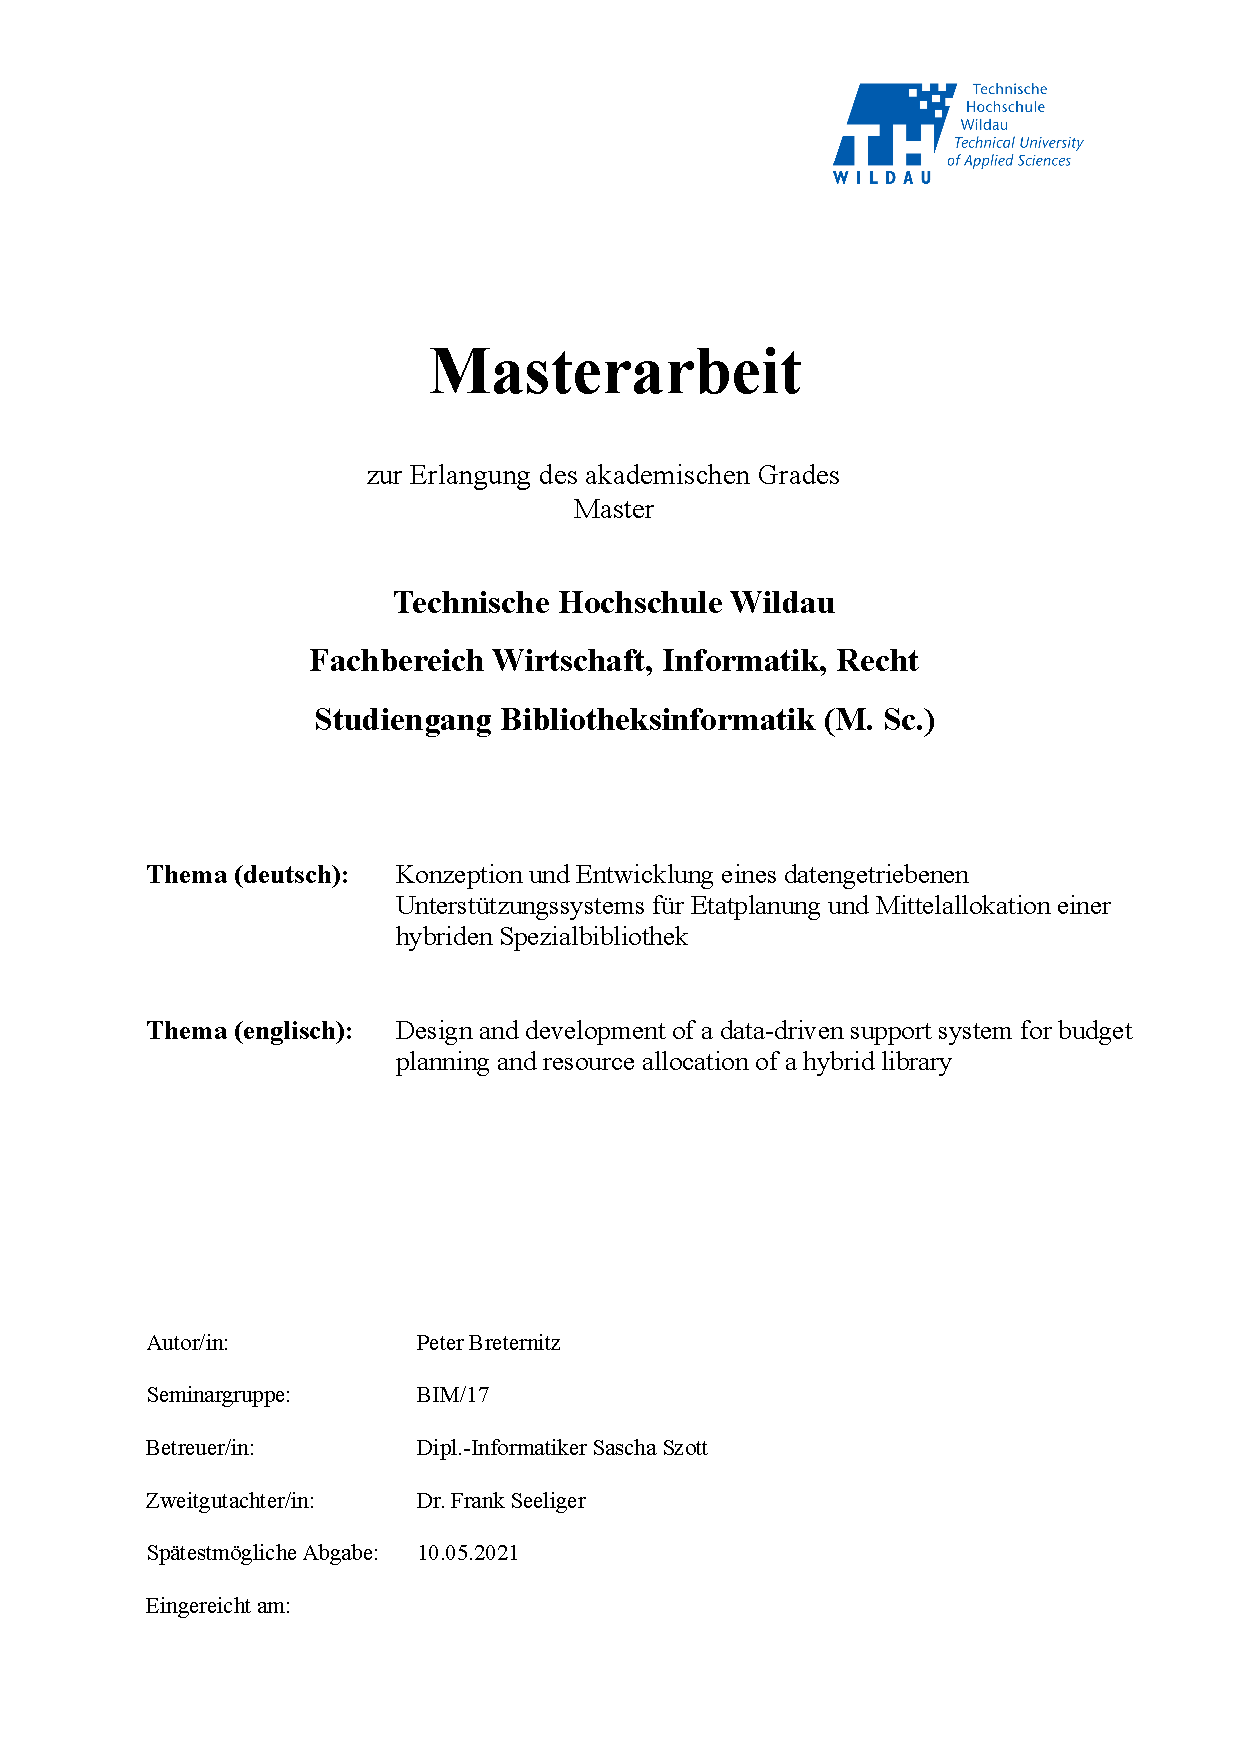
\includepdf{kruscht/pebr1698_2121_cover.pdf}
  \begin{titlepage}
    \vspace*{5cm}
    \makeatletter
    \begin{center}
      \begin{Large}
        \@title
      \end{Large}\\[0.1cm]
      %
      %\begin{Large}
        %\@subtitle
      %\end{Large}\\
      %
      \vspace{0.25 cm}
      \emph{von}\\
      \vspace{0.25 cm}
      \@author
      %
      %\vfill
      %Masterarbeit zur Erlangung des 
      %akademischen Grades\\
      %\emph{Master}\\
      %an der \\
      %\textsc{Technischen Hochschule Wildau}
    \end{center}
    \makeatother
  \end{titlepage}
  
  \newpage
  \null
  \thispagestyle{empty}
  \newpage
  \begin{center}
    \textsc{Zusammenfassung}
  \end{center}
  %
  \noindent
  %
Aufgrund von ökonomischen Entwicklungen müssen Bibliotheken ihr Etat effizient und bedarfsgerecht einsetzen. 
Zudem werden Etatverhandlungen in Bibliotheken immer wichtiger. 
Das Ziel der vorliegenden Masterarbeit war es, ein Proof-of-Concept eines datengetriebenen Unterstützungssystems zur
Etatplanung- und Mittelallokation für die Bibliothek des Max-Planck-Institutes für empirische Ästhetik zu konzipieren und zu entwickeln.
Dafür wurden aus verschiedenen bibliothekarischen Bereichen Daten analysiert 
und ausgewertet. Das datengetriebene Unterstützungssystem ermöglicht die anschauliche Anzeige von wesentlichen Key Performance Indicators wie Budget, 
Umsatz, Ausleihe, Bestandsentwicklung sowie die Lesesaalnutzung in einem Dashboard.
Damit kann die Bibliothek ihre Planung des Etats und den Einsatz der Mittelallokation effizienter und bedarfsgerechter gestalten
sowie Verhandlungen über den Etat sicher führen.

  

\begin{center}
  \textsc{Abstract}
  \end{center}

  \noindent
  %
  Due to economic developments, libraries must use their budgets efficiently and in line with demand. 
  In addition, budget negotiations in libraries are becoming more and more important. 
  The goal of this master thesis was to develop a proof-of-concept of a data-driven support system for
  budget planning and resource allocation for the library of the Max Planck Institute for Empirical Aesthetics.
  For this purpose, data from different library areas were analyzed and evaluated. The data-driven support system 
  displays key performance indicators such as budget, expenditures, circulation, collection development, and reading room usage in a dashboard. 
  This allows the library to plan its budget and allocate funds more efficiently and in line with its needs
  as well as conduct budget negotiations with confidence.
  %\lipsum[1]


  \tableofcontents

%\begingroup
  %\newpage
  %\cleardoublepage
  %\phantomsection
  %\addcontentsline{toc}{chapter}{Tabellenverzeichnis}
  %\listoftables
  %\newpage
  %\cleardoublepage
  %\phantomsection
  %\addcontentsline{toc}{chapter}{Abbildungsverzeichnis}
  %\listoffigures
  %\newpage
  %\cleardoublepage
  %\phantomsection
  %\addcontentsline{toc}{chapter}{Quellcodeverzeichnis}
  %\lstlistoflistings
  %\newpage
  %\cleardoublepage
  %\phantomsection
  %\let\clearpage\relax
  %\glsaddall
  %\printglossary[type=\acronymtype]
  %\newpage
  %\printglossary
  %\newpage
  %\printindex
  %\newpage
%\endgroup

\mainmatter

  %\chapter{Einführung}
Ausgehend von ökonomischen, informationstechnologischen und marktpolitischen Einschnitten in den
vergangenen Jahrzehnten\footnote{Als Gründe zu nennen wären hier: die Explosion der Zeitschriftenpreise im Bereich der
Science, Technology \& Medicine (STM), das Aufkommen von E-Publishing und die Konzentration auf wenige
Verlage},sind Bibliotheken dazu veranlasst, ihr Budget hinsichtlich der Informationsbedarfe
ihrer Nutzer:innen behutsamer zu planen und sich in zunehmenden Maße gegenüber ihren Unterhaltsträgern zu rechtfertigen.

Die Relevanz von bibliothekarischen Kennzahlen ist in diesem Zusammenhang größer geworden.
Deswegen ist es wichtig, Daten aus bibliothekarischen Servicedienstleistungen und Geschäfts-prozessen zu aggregieren, zu erheben und statistisch
auszuwerten, um auf Basis der daraus erzielten Erkenntnisse handeln zu können.

\section{Problemstellung}

\section{Ziel der Arbeit}
Ziel der zu entstehenden Arbeit ist die Entwicklung einer
interaktiven Business-Intelligence-Applikation als proof-of-concept,
mit der systematisch die relevanten Daten einer hybriden Spezialbibliothek aggregiert, statistisch
analysiert und mit geeigneten und modernen Datenvisualisierungstechniken\footnote{Visualisierungen können komplexe Sachverhalte herunterbrechen und
so große Datenmengen - im Gegensatz zu großen Tabellen - leicht verständlich
darstellen. Im Kontext dieser Arbeit konzentriere ich mich auf Ansätze, die Visualisierungen mittels Visualisierungstechniken algorithmisch aus
Daten erzeugen (Informationsvisualisierung, Datenvisualisierung und visuelle Analyse).\cite{RN100}}
ausgegeben werden sollen.
Vor allem soll sich hier auf automatisierte Prozesse zur Gewinnung der Ergebnisse konzentriert werden.

Mit diesen automatisch angefertigten statistischen Datenanalysen sollen zukünftige
Entscheidungen im Bibliotheksmanagement wie Erwerbungspolitik, Budgetplanung und
Mittelallokation hinsichtlich der weiteren Entwicklung der
Servicedienstleistungen evidenzbasiert und datengetrieben unterstützt werden.

Darüber hinaus soll die Applikation  eine Funktion beinhalten, ausgewählte
Resultate automatisiert als \textit{factsheet} zu exportieren, um diese
als Rechenschaftsbericht gegenüber Stakeholdern der Bibliothek präsentieren zu können.

\section{Verwandte Arbeiten}
Es gibt eine Vielzahl kommerzieller Lösungen für den Bibliotheksbereich, die auf Business-Intelligence-Software basieren.
Zu nennen wären \textit{AlmaAnalytics} für das
Next-Generation-Library-System \textit{Alma} von \textit{ExLibris}\footnote{\url{https://www.exlibrisgroup.com/products/alma-library-services-platform/alma-analytics}
Stand: 26.05.2020}, \textit{BibControl} von \textit{OCLC}\footnote{\url{https://www.oclc.org/de/bibcontrol.html} Stand: 26.05.2020},
\textit{CollectionHq} von \textit{Baker \& Taylor}\footnote{\url{https://www.collectionhq.com/} Stand: 26.05.2020} oder \textit{Libinsight} von \textit{SpringShare}\footnote{\url{https://springshare.com/libinsight/} Stand: 26.05.2020}.
Darüber hinaus gibt es Business-Intelligence-Applikationen, die von
Bibliotheken für Reporting, Datenanalyse und Datenvisualisierung adaptiert werden,
wie zum Beispiel \textit{Tableau} von der Firma \textit{Tableau Software} oder
\textit{Crystal Reports} von \textit{SAP}.
Diese Applikationen sind entweder
an bestimmte Bibliothekssysteme zurückgebunden, limitiert in ihren
Funktionen\cite{RN47} oder zu generisch.
Überdies wird sowohl von \textit{HeBis} bzw. von der
Lokal-Bibliothekssystembetreuung als auch von der \textit{mpdl} keine Applikation
in dieser Richtung angeboten.
Ebenso ist ungewiss, wann die Ablösung des schon betagten \textit{CBS/LBS} hin zu
einem neuen Next-Generation-Library-System im \textit{HeBis-Verbund} stattfinden wird und ob
es ein Modul zur statistischen Datenerhebung liefern wird.
Ein gutes Beispiel für ein datengetriebenes Unterstützungssystem findet sich in
der Literatur bei Spielberg, der sich mit dem Thema der Bestandspflege an der
\textit{Universitätsbibliothek Essen} befasst und eine Applikation (weiter-)entwickelt hat, die
die Fachreferent:innen bei der Aussonderung und Erwerbung von Medien
unterstützt.\cite{RN48}
Ebenso finden sich in der Fachliteratur Ansätze, die vorrangig anhand einzelner
Fragestellungen hinsichtlich der Bestandsentwicklung\cite{RN28} oder anderer
bibliothekarischer Servicedienstleistungen\cite{RN43,RN41,RN45} verschiedene statistische Analysen
vollzogen und diese visualisiert haben.
Eine Ausnahme bildet die Entwicklung eines Dashboards an der \textit{New York
University Health Sciences Libraries}, das versucht, möglichst viele Metriken
aus bibliothekarischen Dienstleistungen aufzunehmen.\cite{RN34}
Fast alle Projekte sind an größeren
Universitätsbibliotheken mit ganz unterschiedlichen softwaretechnischen
Herangehensweisen\cite{RN31,RN42} und Zielen\cite{RN1} entstanden.

Dennoch fehlen in der gesichteten Literatur Teile, die sich mit der Budgetierung
befassen und Auskunft über Mittelallokation geben.

Zudem fehlt ein Beispiel in der Literatur, das holistisch alle relevanten Daten, die in den
Geschäftsgängen und Servicedienstleistungen insbesondere einer Spezialbibliothek entstehen,
aggregiert, auf diesen Daten automatisch statistische Analysen ausführt und diese mit modernen Visualisierungstechniken
interaktiv darstellt.

\section{Gliederung der Arbeit}


  \chapter{Einführung}
%Das große Problem\\
Als Ende des Jahres 2019 der Ausbruch der Covid-19-Pandemie begann, entwickelte die 
Johns Hopkins University ein Dashboard als Antwort auf die anhaltende Unsicherheit im Bereich der öffentlichen Gesundheit. 
Dieses visualisiert seit je die gemeldeten Fälle weltweit. Es wurde entwickelt, um Forschern, Gesundheitsbehörden und der breiten Öffentlichkeit 
ein benutzerfreundliches Instrument an die Hand zu geben, mit dem sich der Ausbruch verfolgen lässt. 
Zu dessen Datenquellen gehören unter anderem die Informationen der Weltgesundheitsorganisation, staatliche und nationale
Gesundheitsämter. Die Daten wurden aggregiert und verdichtet. So visualisiert das Dashboard mit einer Landkarte und Punkten den Ausbruch. 
Dazu gibt es Zahlen der bestätigten COVID-19-Fälle, der Todesfälle und  der Genesungen für alle betroffenen Länder\cite[Vgl.][533]{dong_interactive_2020}.

Das faszinierende an dem Dashboard ist, das es gelungen ist, alle relevanten Zahlen auf einer Seite darzustellen
und somit der interessierten Öffentlichkeit schnell einen Überblick zu verschaffen.

\section{Problemstellung}
%Das kleine Problem\\
Ausgehend von ökonomischen, informationstechnologischen und marktpolitischen Einschnitten in den
vergangenen Jahrzehnten, sind Bibliotheken dazu veranlasst, ihr Budget hinsichtlich der Informationsbedarfe
ihrer Nutzer:innen behutsamer zu planen und sich in zunehmenden Maße gegenüber ihren Unterhaltsträgern zu rechtfertigen.
Die Relevanz von bibliothekarischen Statistiken ist in diesem Zusammenhang größer geworden.
Deswegen ist es wichtig, Daten aus den bibliothekarischen Bereichen zu aggregieren, zu erheben und statistisch
auszuwerten, um auf Basis der daraus erzielten Erkenntnisse handeln zu können. 
Die Transparenz von statistischen Daten sorgt für eine bessere Grundlage in den Verhandlungen mit den Stakeholdern
einer Bibliothek. Zudem wird durch sie der Einsatz des Bibliotheksbudgets zielgerichteter auf die Bedürfnisse der Nutzer:innen zugeschnitten.
Dazu ist es zweckmäßig, alle anfallenden Daten für die Budgetplanung und Mittelallokation einer Bibliothek zentral zu sammeln und mit geeigneten 
statistischen Methoden und Verfahren langfristig auszuwerten. Um den Wert dieser aus den Daten gewonnenen Information elegant den Stakeholdern zu kommunizieren und zu präsentieren,
können geeignete Verfahren der Datenvisualisierung zum Einsatz kommen. Die technische Realisierung kann durch gewöhnliche Tabellenkalkulationsprogramme umgesetzt werden.
Um den mitunter hohen Zeitaufwand einerseits zu minimieren und den Automatisierungsgrad hinsichtlich der Aggregation und Auswertung der bibliothekarischen Daten 
andererseits zu erhöhen, können aber auch andere technische Umsetzungen eingesetzt werden. In Bereichen der Wirtschaft kommen sogenannte Business-Intelligence-Systeme zum Einsatz,
die die Entscheidungsfindung auf Grundlage von Unternehmensdaten IT-basiert unterstützen.
%kann geschehen mit herkömmlichen Anwendungen wie Tabellenkalkulationsprogrammen oder mit anderen BI-Systemen...

%Was ist der Markt?\\
%--------------------
Es gibt bereits eine Vielzahl kommerzieller Lösungen für den Bibliotheksbereich, die auf Business-Intelligence-Systemen basieren.
Zu nennen wären \textit{AlmaAnalytics} für das Next-Generation-Library-System \textit{Alma} von \textit{ExLibris}\footnote{\url{https://www.exlibrisgroup.com/products/alma-library-services-platform/alma-analytics}
Stand: 26.05.2020}, \textit{BibControl} von \textit{OCLC}\footnote{\url{https://www.oclc.org/de/bibcontrol.html} Stand: 26.05.2020},
\textit{CollectionHq} von \textit{Baker \& Taylor}\footnote{\url{https://www.collectionhq.com/} Stand: 26.05.2020} oder \textit{Libinsight} von \textit{SpringShare}\footnote{\url{https://springshare.com/libinsight/} Stand: 26.05.2020}.
Darüber hinaus gibt es Business-Intelligence-Applikationen, die von Bibliotheken für Reporting, Datenanalyse und Datenvisualisierung adaptiert werden,
wie zum Beispiel \textit{Tableau} von der Firma \textit{Tableau Software},
\textit{Crystal Reports} von \textit{SAP} oder Microsoft BI.
Diese Applikationen sind entweder an bestimmte Bibliothekssysteme zurückgebunden, limitiert in ihren
Funktionen\cite{golas_statistische_2018} oder zu generisch.
Überdies wird sowohl von \textit{HeBis} bzw. von der
Lokal-Bibliothekssystembetreuung als auch von der \textit{mpdl} keine Applikation
in dieser Richtung angeboten.
Ebenso ist ungewiss, wann die Ablösung des schon betagten \textit{CBS/LBS} hin zu
einem neuen Next-Generation-Library-System im \textit{HeBis-Verbund} stattfinden wird und ob
es ein Modul zur statistischen Datenerhebung liefern wird.

%Wem hilft es?\\
%--------------
Die Notwendigkeit für diese Applikation ist durch das
Fehlen eines zentralen Nachweisortes für bibliothekarische
Statistiken in der Bibliothek gegeben. Da die Bibliothek zudem verschiedene Recherche-Systeme den
Wissenschaftler:innen anbietet, wäre eine Engführung der statistischen
Datenerhebung auf eine Plattform begrüßenswert.
Des Weiteren ist das Erfordernis, bibliothekarische Geschäftsprozesse zu evaluieren und die
Servicedienstleistungen bezüglich der Ziele der Institution noch weiter zu
optimieren, von großer Relevanz. 
Die zu entstehende Applikation könnte hierbei helfen, systematisches Controlling einzuführen und das
Bibliotheksmanagement weiter zu professionalisieren.
%predictive analysis\\


%Warum jetzt?\\
%--------------

Mit dem Ende der Konsolidierungsphase der
Bibliothek, die im Zuge des \textit{Max-Planck-Institutes für empirische
Ästhetik} 2014 gegründet wurde, tritt sie ein in eine Phase, in der ab dem Jahr
2021 Budgetplanungen eine größere Rolle spielen werden.

%Ist das Problem lösbarerer geworden?\\
-------------------\\
Ein System jenseits von Excel zu entwickeln ist heute einfacher geworden, da es einerseits einen Markt für
solche Anwendungen, der im Schatten von DataScience wächst. So muss man kein ausgwachsener FullStack-Entwickler,
um eine Anwendung zu programmieren,
%Wodurch?\\
sondern man kann zurück greifen auf ausgereiftere und mächtige Frameworks
wenig aufwendig Daten statistisch auszuwerten, eher Problem, dass es so viele heterogene Daten aus verschiedenen Datenquellen
gibt die aufbereitet werden müssen. Dashboards gibt es zwar schon lange, sind aber jetzt auch einfacher geworden zu gestalten.
%Was ist der Trend?\\
Ad-hoc Realtime Data - Weg bewegen von schwierig aufsetzen DWH hinzu Data Lakes, die Daten auswerten, wenn sie benötigt werden


\section{Ziel der Arbeit}
%Ihr Ziel der Arbeit in zwei Sätzen.\\
Das Ziel der Arbeit ist die Schaffung eines Dashboards für Budgetplanung in Bibliotheken. 
In Anlehnung an \acrfull{BI}-Systeme soll ein System als proof-of-concept entstehen,
mit dem systematisch die relevanten Daten einer hybriden Spezialbibliothek aggregiert, statistisch
analysiert und mit geeigneten und modernen Datenvisualisierungen ausgegeben werden sollen.
Um künftigen Anforderungen gewachsen zu sein, soll sie
modulbasiert programmiert werden und dadurch leicht erweiterbar und eventuell von
anderen Bibliotheken nachnutzbar sein.

Warum genau dieses Problem?\\
Ist Ihr Beitrag völlig neu, oder nur ein Baustein?\\
Ist Ihr Problem schwer zu lösen oder „straight forward“?\\
eher schwieriger zu lösen, da generischer Ansatz gewählt werden soll -> abstrahieren ein bisschen von konkreter Implementierung
Eher Forschung oder eher Anwendung?\\
eher anwendung
Wenn Sie ein System bauen...\\
Welche Anfragen / Aufgaben wollen Sie beantworten / lösen können?\\
Entwicklung eines Workflows für die Aktualisierung der Daten...
Framework für template design für Daten, die eingespeist werden sollen
Welche Kernfunktionalität soll Ihr System haben?\\
Automatisierte Prozesse bei der Auswertung mit statistischen Verfahren, Import der Daten soll fast vollständig automatisiert sein
Interaktiviät -> Multidemensionalität, Eingrenzung der Zeiträume, Auswählen welche Auswertungen nach Medienart ... Domainwissen
Auswahl aus mehreren Visualisierungen
Bereitstellung der wichtigsten KPI's in einem PDF

Was ist ein typischer (Bedienungs-) Prozess für Ihr System?\\
1) montaliche Budget und Umsatzzahlen kommen als email, werden automatisch in csv umgewandelt -> werden an große csv / datenbank geschrieben
mit der veränderten Datenlage entstehen Veränderungen in den Zahlen -> in Visualisierungen
2) Abfrage des Systems nach Neuerwerbungen mit Systemstellen in der RVK, vierteljahrlich, halbjahrlich, jährlich -> Kontrolle wie und in welchen Systematikgruppen
der Bestand wächst -> RVK-Systematik-Tabelle
Wer nutzt Ihr System, Ihren Algorithmus?\\
Nutzen sollen das System Bibliotheksmitarbeiter:innen und Bibliotheksleitung, auch zum Einspeisen der daten -> Fallback, Fehler abfangen beim Import
Wodurch ist dieses Nutzungsverhalten gekennzeichnet?\\
wenig bis keine Kenntnisse -> soll leicht nutzbar sein ohne große Vorkenntnisse durch automatisierte Prozesse zur Gewinnung der Ergebnisse konzentriert werden.
nur Datei in Ordner schieben
Import/ Export  soll automatisch geschehen.

Anleihen von BI-Systemen in der Architektur, Anhaltspunkte 

Ausleihzahlen nach Jahr, Quartal, Monat
Bestand -> Bestandssegmente(Klass.Gruppen) -> Bestandssegment (einezelne Klassen) -> Einzeltitel => graphisch darstellen
=> Welche Bestandsgruppe am besten geht / schlechtesten

Budgewt



Mit diesen automatisch angefertigten statistischen Datenanalysen sollen zukünftige
Entscheidungen im Bibliotheksmanagement wie Erwerbungspolitik, Budgetplanung und
Mittelallokation hinsichtlich der weiteren Entwicklung der
Servicedienstleistungen evidenzbasiert und datengetrieben unterstützt werden.

Darüber hinaus soll die Applikation  eine Funktion beinhalten, ausgewählte
Resultate automatisiert als \textit{factsheet} zu exportieren, um diese
als Rechenschaftsbericht gegenüber Stakeholdern der Bibliothek präsentieren zu können.

\section{Verwandte Arbeiten}

% Welche Vorarbeiten gibt es schon?\\
% Wo und Wann sind die Vorarbeiten entstanden?\\
% Welche Ziele haben die Vorarbeiten verfolgt?\\
% Auf welche Schwierigkeiten sind sie gestossen?

Ein gutes Beispiel für ein datengetriebenes Unterstützungssystem findet sich in
der Literatur bei Spielberg, der sich mit dem Thema der Bestandspflege an der
\textit{Universitätsbibliothek Essen} befasst und eine Applikation (weiter-)entwickelt hat, die
die Fachreferent:innen bei der Aussonderung und Erwerbung von Medien
unterstützt.\cite{spielberg_eike_t_fachref-assistent_nodate}
Ebenso finden sich in der Fachliteratur Ansätze, die vorrangig anhand einzelner
Fragestellungen hinsichtlich der Bestandsentwicklung\cite{hughes_long-term_2016} oder anderer
bibliothekarischer Servicedienstleistungen\cite{kutlay_shiny_2020, knievel_use_2006,meyer_using_2018} verschiedene statistische Analysen
vollzogen und diese visualisiert haben.
Eine Ausnahme bildet die Entwicklung eines Dashboards an der \textit{New York
University Health Sciences Libraries}, das versucht, möglichst viele Metriken
aus bibliothekarischen Dienstleistungen aufzunehmen.\cite{morton-owens_trends_2012}
Fast alle Projekte sind an größeren
Universitätsbibliotheken mit ganz unterschiedlichen softwaretechnischen
Herangehensweisen\cite{finch_using_2016, wiegand_visualizing_2013} und Zielen\cite{phetteplace_effectively_2012} entstanden.

Dennoch fehlen in der gesichteten Literatur Teile, die sich mit der Budgetierung
befassen und Auskunft über Mittelallokation geben.

Zudem fehlt ein Beispiel in der Literatur, das holistisch alle relevanten Daten, die in den
Geschäftsgängen und Servicedienstleistungen insbesondere einer Spezialbibliothek entstehen,
aggregiert, auf diesen Daten automatisch statistische Analysen ausführt und diese mit modernen Visualisierungstechniken
interaktiv darstellt.

Anwendung kommen deskriptive Statistik, es geht vielmehr darum Daten zusammen zu tragen, als diese zu explorieren 
Abgrenzung deskriptive Statistik / explorative Datenanalyse

\section{Gliederung der Arbeit}
%Wann lesen wir was und warum?\\
Im \autoref{chap:two} werden die theoretischen Grundlagen für die folgenden Kapitel gelegt. Das Kapitel befasst
sich mit den Themen Bibliothek und Statistik, Datenvisualisierung und Business-Intelligence-Systemen. Dabei wird herausgestellt, wie wichtig Statistik
im bibliothekarischen Bereich sind, was Datenvisualisierungen sind und warum sie eingesetzt werden sollen und welche Anleihen Business-Intelligence-Systeme 
für das zu entstehende System liefern können. \autoref{chap:three}
wird die Bibliothek vorgestellt und darauf eingegangen welche bibliothekarischen Statistiken bereits erhoben wurden.
Nachdem die Ausgangssituation bestimmt wurde, wird mit der Anforderungsanalyse im \autoref{chap:four} die Konzeption einer Lösung vorgestellt.
Im \autoref{chap:five} wird die Umsetzung diskutiert. Bevor das System bewertet wird, wird das Design und die Implementierung vorgestellt.
Das Fazit wird im \autoref{chap:six} mit dem Stand der Umsetzung, den lessons learned und einem Ausblick auf Themen, die noch bearbeitet werden könnten, gezogen.

  \chapter{Theoretische Grundlagen}
\label{chap:two}
In diesem Kapitel wird der theoretische Rahmen für die weiteren Kapitel gelegt. Im
ersten Abschnitt werden die Grundlagen der Budgetplanung und Mittelallokation im Zusammenhang mit bibliothekarischen Statistiken erläutert. 
Der darauf folgende Abschnitt handelt von Datenvisualisierungen und deren Einsatz
für Datenrepräsentationen und Datenpräsentation. Abschließend wird das Modell der Business-Intelligence-Systeme als Schmelzpunkt der 
beiden vorangegangen Kapitel eingeführt.

\section{Bibliothek und Statistik}
\label{chap:two_one}
% Bibliotheksrahmen - Etatplanung - Etatbedarfe, Zielsetzung der Bibliothek
Die Etatplanungen von Bibliotheken richten sich nach deren Informations- und Versorgungsauftrag. 
Seit Beginn der 1990er Jahre müssen sich Bibliotheken mit den Auswirkungen einer veränderten Medienlandschaft auseinandersetzen.
Sie kämpfen mit dem größer werdenden Informationsangebot, den steigenden Preisen auf dem Publikationsmarkt, 
den zunehmenden Kommerzialisierungstendenzen in der Verlagslandschaft und den neuen Medientypen. 
Zu nennen wären hier konkret: die Explosion der Zeitschriftenpreise im Bereich der \acrfull{STM}, die Konzentration auf wenige Verlage, 
und dem Aufkommen von Ebooks. Demgegenüber steigen Bibliotheksetats nur mäßig. 
Somit geht ein Kaufkraftverlust einher \cite[vgl.][164 ff.]{moravetz-kuhlmann_monika_erwerbungspolitik_2015}.
Diese Entwicklung betrifft nicht nur Universitätsbibliotheken, sondern auch Spezialbibliotheken von Forschungseinrichtungen.
Bibliotheken haben Instrumente entwickelt, um den Informationsauftrag trotz dieser Widrigkeiten zu erfüllen.
So entstehen seit Mitte der 1990er Jahre von Bund und Ländern geförderte Konsortien, um den Kostendruck auf Bibliotheken im Bereich der elektronischen
Fachinformationen zu mildern. Neue Geschäftsmodelle werden zur Abfederung der Kosten entwickelt, um Preisnachlässe bei den Verlagen zu erzielen
\cite[vgl.][169 ff.]{moravetz-kuhlmann_monika_erwerbungspolitik_2015}. Das Projekt \textit{Deal} -- ein Projekt der Hochschulrektorenkonferenz (HRK) in Zusammenarbeit mit den
wissenschaftlichen Einrichtungen in Deutschland -- konnte so in den vergangenen Jahren Verträge mit den Verlagen \textit{Springer} und \textit{Wiley} erfolgreich abschließen \cite[vgl.][]{projekt_deal_projekt_2020}.

Um den Veränderungen des Publikationsmarktes lokal in der Bibliothek zu begegnen, wird es immer wichtiger, das Bibliotheksbudget und die Mittelallokation kosteneffizient zu planen. 
Dies geschieht bisher in größeren Bibliotheken durch Etatbedarfs- und Etatverteilungsmodelle \cite[vgl.][172 ff.]{moravetz-kuhlmann_monika_erwerbungspolitik_2015}.
%Ziel dieser Modelle ist die effiziente Mittelallokation 
% transparente und gerechte Verteilung knapper Ressourcen% innerhalb der Bibliothek. 
% Mittelallokation bezeichnet die Verteilung knapper Ressourcen. 
Diese Modelle basieren auf der statistischen Erhebung von bibliothekarischen Kennzahlen.

%Was ist Statistik\\
%hat schon immer große Rolle in Bibliotheken gespielt\\
%BIX, Deutsche Bibliotheksstatistik (seit wann)\\
Bibliotheksstatistik reflektiert das Gestern, Heute und Morgen, indem 
sie die bibliothekarischen Servicedienstleistungen evaluiert und den zukünftigen Zielen und Aufgaben anpasst \cites[vgl.][2 f.]{jilovsky_cathie_library_2004}[vgl.][462]{laitinen_markku_library_2013}.
Im deutschen Bibliothekswesen gibt es die umfangreiche \acrfull{DBS}. 
Träger der \textit{\acrshort{DBS}} sind das \acrfull{hbz NRW},  das \acrfull{KBN}, die \acrfull{KMK} sowie den teilnehmenden Bibliotheken.
Aufgabe der \textit{\acrshort{DBS}} ist die jährliche statistische Datenerhebung von Bibliothekskennzahlen. 
Seit 1999 werden die Daten nur noch online erfasst, ausgewertet und präsentiert \cite[vgl.][2]{schmidt_deutsche_2008}.
Neben anderen Servicedienstleistungen bietet die \textit{\acrshort{DBS}} Gesamtauswertungen an.
%Dennoch ist die \textit{\acrshort{DBS}} vielmehr eine Datengrundlage für die Auswertung der Daten als eine Auswertung solcher.
Daneben gab es den \acrfull{BIX}, der ursprünglich für die Leistungsmessung in Öffentlichen Bibliotheken konzipiert wurde. 
2002 wurde er erweitert auf das Wissenschaftliche Bibliothekssystem. Der \textit{\acrshort{BIX}} wurde 2015 aufgrund von Finanzierungsproblemen eingestellt. 

%Erhebung von qualitativen und quantitativen Daten Bsp.:\\
Bibliothekarische Kennzahlen werden durch quantitative und qualitative Evaluationsverfahren erhoben. Diese Verfahren
sind auf den Bestand der Bibliothek zentriert. 
Bestand ist nach Johannsen und Mittermaier
\textquote{... die Gesamtheit aller Medien, die eine Bibliothek ihren Nutzern anbietet, sei es, dass sie diese 
„physisch“ besitzt, sei es, dass sie entsprechende Nutzungsrechte erworben hat.} \cite[252]{johannsen_jochen_bestands-_2015}.
Als Typen der Bestandsevaluation sind sammlungs-, nutzungsbezogene und nutzer:innenbezogene Evaluationen zu nennen.\cite[vgl.][302]{johnson_peggy_fundamentals_2014}
Basieren die sammlungs- und nutzungsbezogene Evaluation auf quantitativen Daten, greift die nutzer:innenbezogene Evaluation zumeist auf qualitative Daten zurück. 
\cite[vgl.][461 ff.]{blake_data_2004}.

Die sammlungsbezogene Evaluation betrifft die Größe des Bestandes und das Wachstum über die Jahre. Die Bestimmung der Bestandsstärke- und tiefe, 
der Ausgewogenheit in den Bestandssegmenten sind Ziele der sammlungsbezogenen Evaluation. 
Ebenfalls lässt sich die Frage nach der aktuellsten Literatur im Bestand oder in einem Segment durch die sammlungsbezogene Evaluation klären.

Nutzungsbezogene Evaluation umfasst die Lesesaalnutzung, die Ausleihe vor-Ort, die Nutzung des Fernleihservices oder Dokumentenlieferdienste und die Online-Nutzung von elektronischen Ressourcen \cite[vgl.][254 ff.]{johannsen_jochen_bestands-_2015}.
Die Frage nach den Zugriffsstatistiken auf elektronischen Ressourcen beansprucht in der nutzungsbezogenen Evaluation einen größer werdenden Raum.
Die internationale Organisation \textit{\acrfull{COUNTER}} gibt dazu die COUNTER-Statistiken heraus. Mitglieder der Organisation sind Verlage, Bibliotheken
und Zwischenhändler. Die COUNTER-Statistiken sind mittlerweile der Quasi-Standard für die Zugriffsstatistiken 
auf elektronische Ressourcen geworden. Diese werden getrennt nach Art der Informationsressourcen in verschiedenen Reports herausgegeben. \cite[vgl.][260 ff.]{johannsen_jochen_bestands-_2015}. 
Mittlerweile ist die fünfte Iteration der COUNTER-Statistiken \textit{\acrshort{COP 5}} erschienen \cite[vgl.][]{counter_abstract_2020}.
%Im Jahr 2019 ersetzte sie die vorhergehende Version.
Die Bibliotheken sind bei dem Bezug von diesen Statistiken auf die Unterstützung der Verlage angewiesen. Diese stellen unregelmäßig die \textit{\acrshort{COP 5}}-Statistiken zur
Verfügung. Ziele der nutzungsbezogenen Evaluation sind die Identifizierung von ausleihträchtigen Medienbeständen (Vormerkungs- und Rennerlisten) und
die Deakquisition schlecht oder gar nicht genutzter Titel. Ebenso kann die Evaluation von Fernleih- und Dokumentenlieferungen Hinweise auf Bestandslücken liefern
\cite[vgl.][255 ff.]{johannsen_jochen_bestands-_2015}. Als Konsequenz aus den COUNTER-Statistiken kann die Abbestellung von elektronischen Ressourcen resultieren.

Die nutzer:innenbezogene Evaluation ist auf den Nutzer:innenkreis der Bibliothek und deren Informationsbedürfnisse zentriert. 
%Fundamental ist der Unterschied zwischen den einzelnen Evalationsverfahren in der Erhebung der Daten. 
Die sammlungs- und nutzungsorientierten Evaluationsverfahren basieren auf der Erhebung von quantitativen Daten wie der Bestandsgröße oder der Anzahl von Ausleihen. 
Nutzer:innenbezogene Evaluation benutzt qualitative Daten, die sie aus Befragungen erhebt.
%Warum ist Messbarkeit von bibliothekarischen Daten wichtig?\\
%Welchen Impact für Budgetplanung können statistische Daten haben?\\

Die einzelnen Evaluationen vermitteln ein realistisches Gesamtbild der Bibliothek und deren Service-Dienstleistungen. 
Die datengetriebenen Evalutionsauswertungen bieten Hinweise auf Optimierungen der bibliothekarischen Service-Dienstleistungen. 
Die Auswertungen können durch die Bibliotheksleitung aufgenommen werden und in strategische (zukünftige) Entscheidungen einfließen. 
So kann ein detailliertes Erwerbungsprofil und somit eine gezieltere Erwerbungspolitik entstehen. 
Dadurch wird das Management der Ressourcen effektiver und effizienter \cite[vgl.][297]{johnson_peggy_fundamentals_2014}.
Gegenüber Stakeholdern kann auf der Grundlage der Evaluationen gezielt um Budget verhandelt werden.
\begin{displayquote}
    The purpose of the statistics is to give the management of the library or another decision-maker 
    a satisfactory and correct picture about the situation of the library as a support to them - the statistics are the mirror of the library!
    \cite[463]{laitinen_markku_library_2013}
\end{displayquote}

Um ein zufriedenstellendes und korrektes Bild der Situation der Bibliothek zu präsentieren, helfen sorgsam ausgewählte Datenvisualisierungen.



\clearpage
\section{Datenvisualisierung}
\label{chap:two_two}
Datenvisualisierungen sind wirkmächtig. Sie stellen einen Weg da, statistische Informationen effizient zu kommunizieren \cite[vgl.][15]{Tufte01}, 
indem sie Daten mit visuellen Reizen ausstatten, die vom menschlichen Auge aufgenommen und vom menschlichen Gehirn schnell verarbeitet werden können \cite[vgl.][32]{few_now_2009}. 
Zusammenhänge, Trends und Ausnahmen einer großen Datenmenge sind in einer Zahlenkolonne schwieriger zu entdecken als mit einer geeigneten Datenvisualisierung.
Datenvisualisierungen ermöglichen den visuellen Vergleich von verschiedenen Informationen. Sie können  eine große Anzahl von Datenpunkten kompakt darstellen. 
Datenvisualisierungen können nicht nur die Informationen von verschiedenen Blickwinkeln anzeigen, sondern die Informationen auch
mit unterschiedlicher Granularität darstellen \cite[vgl.][245]{muller_business_2013}.
% Dort sind Zusammenhänge zunächst nicht sichtbar und müssen erst kognitiv erarbeitet werden. 

Visualisierungen benötigen Daten. Daten benötigen Visualisierungen, um ihren Wert besser präsentieren zu können \cite[vgl.][16]{kirk_data_2019}.
Im folgenden werden der inhaltliche Bezugsrahmen und die Merkmale von Datenvisualisierungen näher erläutert.

%Mit leistungsstarken Computern und einer großen Datenvielfalt, lassen sich heutzutage Grafiken, die Daten von verschiedenen Blickwinkeln betrachten, erstellen.  
%Warum Datenvisualisierungen wichtig sind, was sie unterstützen können. Warum es einfacher ist auf ein Diagramm zu schauen als auf eine Tabelle voller Daten
%Unterlegen Daten mit visuellem Reiz der vom Auge  aufgenommen und vom Gehirn schneller verarbeitet werden kann.
%Wirkmächtiger ein 2 dimensionales Diagramm als eine Tabelle mit 1000 von Werten. Für jeden einzelnen Wert kann 
%Nicht neu, aber heutzutage mit dem leistungsstarken Computern und der großen Datenvielfalt lassen sich einfach schnell Datenvisualisierungen erzeugen
%Machine Learning 
%

Datenvisualisierungen sind Verfahren der deskriptiven und explorativen Statistik beziehungsweise der explorativen Datenanalyse. 
Im Allgemeinen bilden sowohl die deskriptive Statistik als auch die explorative Datenanalyse keine Hypothesen. Beide treffen nur Aussagen zu vorliegenden Datensätzen. 
Dennoch gibt die explorative Statistik Hinweise für eine mögliche Hypothesenbildung in der weiterführenden Analyse. 
Da sich die explorativen Verfahren besonders für große Datenmengen eignen, fand mit der rasanten Entwicklung der Informationstechnologien 
eine starke Verbreitung dieser Verfahren in den vergangenen Jahren statt. Die Datenvisualisierung hat sich aus den explorativen Verfahren zu einem eigenständigen Fachgebiet der Statistik 
beziehungsweise der Informatik entwickelt \cite[vgl.][28 f.]{becker_stochastische_2016}. Dies belegt auch eine Vielzahl von Fachliteratur, die in den letzten Jahren veröffentlicht wurden.
%\textquote{Furthermore of all methods for analyzing and communicating statistical information, well-designed data graphs
%are usually the simplest and at the same time the most powerful}\cite[vgl.][Introduction]{Tufte01}
%\textquote{...the efficient communications of complex quantitative ideas}\cite[vgl.][15]{Tufte01}
%Im Gegensatz zur Inferenzstatistik ist die Aufgabe der Deskriptiven
%Statistik die Gewinnung von Information aus Daten. Dazu werden verschiedene statistische Verfahren beziehungsweise Methoden angewendet. 
%Datenvisualisierungen sind solche Verfahren.
%Datenvisualisierungen sind statistische Verfahren der Deskriptiven und der Explorativen Statistik.
%\cites[vgl.][3]{cleff_deskriptive_2011}[vgl.][7 ff.]{coolidge_statistics_2021}.


Der Begriff der Datenvisualisierung umschreibt die visuelle Repräsentation und Präsentation von Daten, um das Verständnis zu verbessern \cite[vgl.][15 ff.]{kirk_data_2019}.
% Ähnlich der Definition von \Citeauthor{kirk_data_2019} ist Datenvisualisierung nach \citeauthor{Cairo} 
%Oberbegriff für Informationsvisualisierung / Scientific Visualization\\
Er wird in Teilen der Literatur als Oberbegriff für \textquote{\textit{Information visualization}} und 
\textquote{\textit{Scientific Visualization}} verwendet \cite[vgl.][11]{few_now_2009}.
% Abgrenzung zu Infographics
%Datenvisualisierung grenzt sich in Form und Inhalt von dem Begriff der Infographik ab. 

% Was ist unter Datenvisualisierung zu verstehen?\\
Datenvisualisierungen haben das Ziel, die Analyse, Exploration und Entdeckung der Daten zu ermöglichen. Sie sollen das Verständnis der dargestellten Daten erleichtern
und sind anders als Infographiken\footnote{Infographiken haben die Aufgabe Nachrichten zu kommunizieren.
Sie bestehen aus einer Mischung von Diagrammen, Karten, Illustrationen und Text. Klarheit und Tiefe der Darstellungen sind dabei wichtig
\cite[vgl.][31]{cairo_truthful_2016}. Sie werden auch als \textquote{\textit{Explanation Graphics}}
bezeichnet und bestimmen sich dadurch, dass sie Geschehen und Ereignisse graphisch darstellen. 
Historisch sind Infographiken mit dem Medium der Printzeitungen und Printzeitschriften verbunden \cite[vgl.][27]{kirk_data_2019}.}
nicht primär dafür geschaffen, Geschichten über die Informationen zu erzählen \cite[vgl.][20 ff.]{kirk_data_2019}. 
Sie werden vielmehr als Werkzeuge verstanden, die es ermöglichen sollen, Entscheidungen aus den visualisierten Daten zu ziehen \cite[vgl.][31]{cairo_truthful_2016}. % -> Sind Daten dargestellt > Exploration der Daten
% Mit der visuellen Darstellung kann die Exploration dieser beginnen und bietet Raum für neue Zusammenhänge...

In der Fachliteratur finden sich verschiedene Eigenschaften von Datenvisualisierungen. \Citeauthor{cairo_truthful_2016}
führt fünf Eigenschaften auf: \textit{truthful}, \textit{functional}, \textit{beautiful}, \textit{insightful} und \textit{enlightening}.
Datenvisualisierungen basieren auf gründlicher und ernsthafter Forschung (truthful). Sie sind funktional, dass heißt
sie bemühen sich die Daten genau darzustellen (functional). Indem Datenvisualisierungen schwer entdeckbare Beweise offenbaren, 
sind sie aufschlussreich (insightfull). Darüber hinaus sollen sie für die Zielgruppe attraktiv sein (beautiful).
Zudem sind Datenvisualisierungen aufklärend (enlightening), da sie Veränderungen im Denken anstoßen können \cite[vgl.][45]{cairo_truthful_2016}. 
%Ferner sollen sie computerunterstützt und interaktiv sein \cite[vgl.][12]{few_now_2009}.

Die visuelle Repräsentation der Daten erfolgt unter Verwendung graphischer Markierungen (marks) wie Punkt-, 
Linien und Balkensymbolen. Die Eigenschaften dieser Markierungen wie ihre Form, Größe oder Farbe kodieren die
darunter liegenden Datenwerte. Die so kodierten Datenwerte werden dann in Diagrammen dargestellt \cite[vgl.][135 ff.]{kirk_data_2019}.
%Mit dem Einsatz dieser visuellen Elemente sollen Muster, Trends und Ausnahmen in Daten leichter sichtbar gemacht werden.

%Datenvisualisierungen setzen einen visuellen Reiz, der schneller vom menschlichen Auge verarbeitet werden kann \cite[vgl.][32]{few_now_2009}.

%Deswegen sind mit dem Einsatz der visuellen Elemente Muster, Trends und Ausnahmen in den Daten leichter erkennbar.
% Zweck der Datendarstllung Bindung an Daten
%Ein diskretes Merkmal kann auf Basis der natürlichen Zahlen abzählbar viele Merkmalsausprägungen (values) annehmen. Die Bestandsgröße einer
%Bibliothek ist ein diskretes Merkmal. Im Gegensatz dazu können die Merkmalsausprägungen eines stetigen Merkmals jeden beliebigen Wert annehmen. 
%So ist die Raumtemperatur ein stetiges Merkmal.
% Welchen Zweck? Für wen?
Die visuelle Datenrepräsentation wird von verschiedenen Faktoren beeinflusst.
% Datentyp
Grundsätzlich ist zu überlegen, ob die Daten in Diagrammen oder Tabellen repräsentiert werden sollen.
Daran anschließend ist die Frage zu klären, welche Art der Beziehung zwischen den Daten gezeigt werden soll.
Für die Auswahl der Diagramme ist es wichtig zu bestimmen, ob es sich zum Beispiel um einen Kategorienvergleich, eine Zeitreihe, eine Rangfolge, 
eine relative Häufigkeit oder eine Korrelation handelt \cite[vgl.][137]{few_show_2012}.

Für die Auswahl der richtigen Datenvisualisierung sind des Weiteren die unterschiedlichen Datentypen von großer Relevanz.
Datentypen \textquote{...define the nature of the values held under each variable and about each item 
in your dataset.} \cite[99]{kirk_data_2019}.  Eine Variable (Merkmal) kann qualitativ (kategorial) oder quantitativ (metrisch) sein.
Die \autoref{fig:data types} zeigt die statistischen Datentypen nach der \acrfull{NOIR} 
\cite[vgl.][12 ff.]{bortz_statistik_2010} mit den möglichen Aussagegehalten und Beispielen.
\footnote{Manchmal ist auch nur die Unterscheidung zwischen nominalen, ordinalen und metrischen
Merkmalen in der wissenschaftlichen Literatur anzutreffen \cite[vgl.][20]{cleff_deskriptive_2011}. 
Unter Berücksichtigung der großen Vielfalt (variety) der Daten, schlägt \Citeauthor{kirk_data_2019} 
eine Erweiterung der \acrshort{NOIR}-Systematik um einen textuellen Datentyp vor \cite[vgl.][100]{kirk_data_2019}.}

 
 \begin{figure}[h]
    \centering
        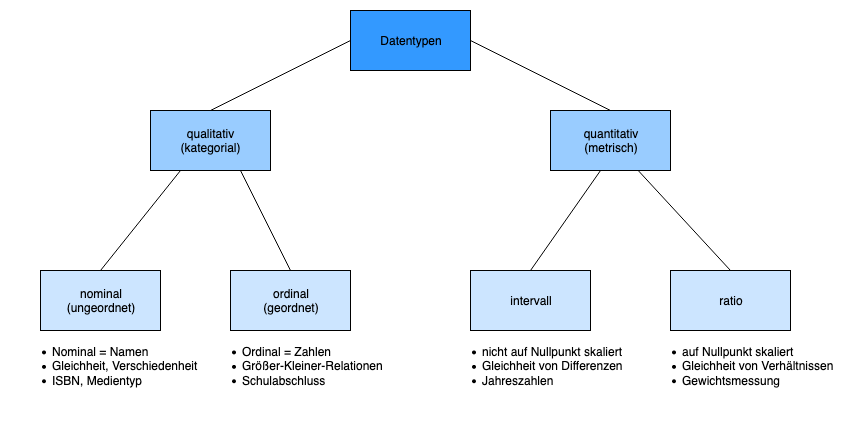
\includegraphics[width=12cm]{dt}
        \caption{Statistische Datentypen mit Aussagegehalten und Beispielen}
        \label{fig:data types}
\end{figure}


%Nominale Datentypen können auch Ziffern beinhalten. 
Unterschieden werden die Merkmale ferner nach diskret und stetig.
Ein diskretes Merkmal kann auf der Basis der natürlichen Zahlen abzählbar viele Merkmalsausprägungen annehmen.
So ist zum Beispiel die Größe des Medienbestandes einer Bibliothek ein diskretes Merkmal, da es keine halben oder viertel Medien gibt.
Im Gegensatz dazu können die Merkmalsausprägungen eines stetigen Merkmals jeden beliebigen Wert annehmen. So ist zum Beispiel die Raumtemperatur ein stetiges Merkmal.
Qualitative Merkmale können nur diskret sein, während quantitative Merkmale sowohl diskret als auch stetig sein können. 
Für kategoriale Merkmale eignen sich Balken- und Kreisdiagramme eher als Liniendiagramme, da kategoriale Daten nur diskret sein können.
%Für quantitative Merkmale eignen sich  Balken- und Liniendiagramme???

Der Einsatz von Datenvisualisierungen wird ebenfalls bestimmt von der Größe der Datenmenge.
Die Darstellung einer großen Datenmenge kann zum Beispiel durch die Wahl eines bestimmten Diagrammes überladen wirken. 
So stößt die Darstellung einer Datenmenge mit vielen Kategorien durch Balken- und Kreisdiagramme 
in der Übersichtlichkeit an Grenzen und kann den Wert der zu erzielenden Aussage verwischen. 

Daten können mit mit Softwareprogrammen wie Microsoft Excel oder anderen Tabellenkalkulationsprogrammen visualisiert werden.
In Data-Science-Projekten können ebenfalls verschiedene Frameworks zum Einsatz. Populär sind die Bibliotheken Matplotlib, Seaborn, Plotly für 
die Programmiersprache Python. Für die Programmiersprache R gibt es ebenfalls vielfältige Möglichkeiten der Visualisierung mit
ggplot. Einen guten Überblick erhält man auf der Webseite \textquote{The Chart maker}\footnote{\url{https://chartmaker.visualisingdata.com/} Stand: 17.09.2020}.
Eine mächtige und verbreitete Javascript-Bibliothek zur Datenvisualisierung ist D3.js.
%Interaktivität


Die dargestellten Daten kommen aus allen Bereichen des Lebens. Daten entstehen in wissenschaftlichen Experimenten, aus statistischen Erhebungen wie 
dem Census, auf Kassenzetteln, in Smartphones, in Unternehmen oder in Einrichtungen wie Bibliotheken. 
In Unternehmen werden Datenvisualisierungen eingesetzt, um auf der Managementebene die operative Planung und Entscheidungsfindung zu unterstützen.
Dabei sind Datenvisualisierung ein Bestandteil eines ganzheitlichen Prozess, der unter dem Begriff \acrfull{BI} fungiert. Dieser scheint mittlerweile auch im Bibliothekswesen angekommen zu sein.


%DV für Teile der Daten -> Dateln liegen überall im Unternehmen verstreut in einzelnen Abteilungen
%Teilweise ausgewertet -schwierig für Berichtswesen gegenüber Stakeholdern
%Lsg. wäre eine ganzheitliche IT-Lösung. Diesen Ansatz fährt BI
%Die Präsentation der Daten füe wen ... umschließt Interaktivität -> statischen Bildern hinzu interaktiven \dots
%audience -> stakheoldern -> Berichtswesen oder BI
%zu welchen Zweck -> ...was die Daten beinhalten welche Indikatoren
%Datenvisualisierungen lassen sich bündeln 
%Präsentation den Stakeholdern, um datengetrieben Managemententscheidungen zu erleichtern
%bieten sich BI
%Neuere Entwicklung gehen hinzum Dashboard  - einer Darstellung der wesentlichen Informationen komprimiert \dots
%Dashboards können  als Teil von Business-Intelligence-Systemen verstanden werden.


\section{Business-Intelligence-Systeme}
\acrfull{BI}\footnote{Synonym wird auch manchmal der Begriff Analytische Informationssysteme oder Business-Intelligence-Systeme gebraucht}
bezeichnet allgemein Konzepte und Methoden zur Entscheidungsfindung, die auf
erfassten Informationen beruhen. 
%Aus technischer Sicht umfasst \textit{\acrshort{BI}} unter anderem die Komponenten der Datenhaltung,der  Datenintegration, des Reportings, die \acrfull{OLAP} und Data Mining.
\textit{\acrshort{BI}-Systeme} gehören zu den Management-Support-Systemen, die seit den 1960er Jahren in Unternehmen im Einsatz sind \cite[vgl.][83]{gronwald_integrierte_2020}.

Populär wurde der Begriff der \textit{\acrshort{BI}} in den 1990er Jahren. Die Verbreitung von \textit{\acrshort{BI}} fiel zusammen mit der 
Entwicklung einheitlich strukturierter und dauerhaft verfügbarer Datenbanken in Unternehmen, sogenannten Data Warehouses (DWH).
Grund für diese Entwicklung waren die immer neuen Informationsbedürfnisse auf Managementebene, 
die schnell befriedigt werden sollten 
%\cite[vgl.][268 f.]{abts_grundkurs_2017}. 
Die Einrichtung dieser Datenbanken zielt ab auf eine umfassende Informationsversorgung durch Verdichtung der Unternehmensdaten 
%auf unterschiedlichen Schichten mit detaillierten Kennzahlen. 
%Der Zugriff auf diese Informationen soll jederzeit erfolgen 
\cite[vgl.][267 ff.]{abts_grundkurs_2017}. 

\textit{\acrshort{BI}} beschreibt einen integrierten, unternehmensspezifischen,
IT-basierten Gesamtansatz zur Unterstützung betrieblicher Entscheidungen \cite[vgl.][270]{abts_grundkurs_2017}. 
Ein Hauptmerkmal der \textit{\acrshort{BI}} ist nach \Citeauthor{linden_geschaftsmodellbasierte_2016} die Entscheidungsunterstützung der Managementebene
\cite[vgl.][111]{linden_geschaftsmodellbasierte_2016}. Die Abgrenzung zu operativen
Anwendungssystemen wie \acrfull{OLTP}-Systemen ist laut \citeauthor{abts_grundkurs_2017} ein weiteres wichtiges Merkmal der \textit{\acrshort{BI}}-Systeme \cite[vgl.][267]{abts_grundkurs_2017}. 

Die wesentlichen Schichten eines \textit{\acrshort{BI}-Systems} umfassen die Bereiche der internen und externen Datenlieferanten, den Komplex der Datenintegration- und aufbereitung, 
das Gebiet der Datenspeicherung - und bereitstellung im \textit{\acrlong{DWH}} und den Zweig der Datenanalyse und -präsentation\cites[vgl.][126 ff.]{linden_geschaftsmodellbasierte_2016}[vgl.][8]{kemper_business_2010}. 

Die Schichten der \textit{\acrshort{BI}-Systeme} können in einem Referenzarchitekturmodell abgebildet werden. 
%Dieses Modell kann alle technischen Komponenten umfassen, die von der eigentlichen konkreten Implementierung abstrahiert werden müssen. 
Die Referenzarchitektur kann auch die Datenflüsse zwischen den verteilten Systemeinheiten und Komponenten erfassen \cite[vgl.][126 ff.]{linden_geschaftsmodellbasierte_2016}.
Eine schematische Darstellung in Form eines solchen Referenzarchitekturmodell \autoref{fig:bis}.
%In der Fachliteratur wird das Modell oft mit drei Ebenen beschrieben\cites[vgl.][126 ff.]{linden_geschaftsmodellbasierte_2016}[vgl.][8]{kemper_business_2010}.

\begin{figure}[h]
    \centering
        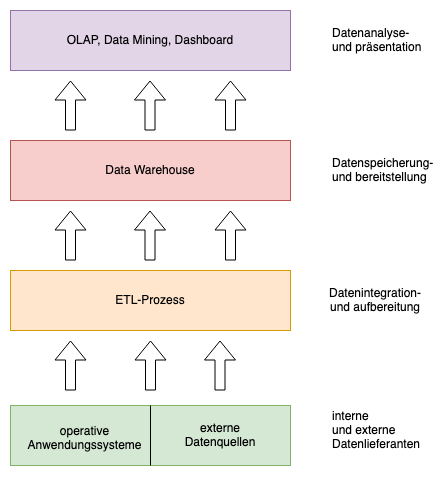
\includegraphics[width=12cm, height=12cm]{bis}
        \caption{Schichten eines Business-Intelligence-Systems}
        \label{fig:bis}
\end{figure}

%Die Ebenen umfassen die Ebene der Datenquellen und Datenerfassung, die Ebene der Datenbereitstellung und Speicherung sowie die Ebene der Datenanalyse und -präsentation.
Von den internen und externen Datenlieferanten werden die Daten im Bereich der Datenintegration- und aufbereitung mithilfe von \acrfull{ETL}-Prozessen bearbeitet. 
%Der letzte genannte Bereich wird auch als Staging Area bezeichnet.
In einem ersten Schritt werden die Daten aus den \textit{\acrshort{OLTP}-Systemen} oder aus anderen Datenquellen extrahiert. 
Der anschließende Transformationsprozess wandelt die Daten in ein homogenes Format um. Dabei handelt es sich um einen vierstufigen Prozess. Die Daten werden mit Hilfe 
zum Teil automatischer Verfahren bereinigt, harmonisiert, verdichtet (aggregiert) und angereichert.
Bereinigt werden die Daten unter anderem von syntaktischen und semantischen Mängeln. Unterschiedliche Codierungen der Daten werden durch die Harmonisierung 
beseitigt. Des Weiteren werden die Daten verdichtet, d.h. es werden Summationen von den Daten auf verschiedenen Ebenen durchgeführt und gespeichert. 
Die Berechnung und Speicherung wichtiger Kennzahlen geschieht durch das Verfahren der Anreicherung \cites[Vgl.][86]{gronwald_integrierte_2020}[vgl.][277 f.]{abts_grundkurs_2017}.
Schließlich werden die Daten in einem Ladeprozess in das \textit{\acrlong{DWH}} geladen \cite[vgl.][129 ff.]{linden_geschaftsmodellbasierte_2016}. 

Die Datenspeicherung und -bereitstellung erfolgt im \textit{\acrshort{DWH}}. Dieser Bereich ist nach \citeauthor{linden_geschaftsmodellbasierte_2016} zentral für die 
\textit{\acrshort{BI}-Systeme}. Ein \textit{\acrlong{DWH}} ist ein logisch zentralisiertes Datenhaltungssystem. Dieses ist physisch 
von den operativen Anwendungssystemen getrennt und stellt eine harmonisierte Datenbasis für betriebswirtschaftliche Analysen bereit.\footnote{Alternativen zum Data Warehouse wären verschiedene Data Marts, 
die kleinere Datenspeichereinheiten darstellen und sich inhaltlich an späteren Abfrage- und Auswertungszwecken orientieren.} 
Ein \acrlong{DWH} zeichnet sich durch die vier Merkmale themenorientiert, zeitorientiert, integriert und nicht-volatil aus. Die Speicherung der Daten erfolgt nach Themenschwerpunkten und
orientiert sich am Informationsbedarf des Unternehmens. Die zeitorientierte Speicherung der Daten ermöglicht Zeitreihenanalysen auf historischen Daten. Die Integration der Daten aus verschiedenen heterogenen
externen und internen Datenquellen eines Unternehmens zur Schaffung einer homogenen Datenbasis ist ein wichtiges Charakteristikum des \textit{\acrlong{DWH}} \cite[Vgl.][136]{linden_geschaftsmodellbasierte_2016}

Die Datenintegration in das \textit{\acrlong{DWH}} kann auf Grundlage eines multidimensionalen Datenmodells erfolgen. Ein \textit{\acrshort{DWH}} ist üblicherweise nach einem Datenwürfel (data cube) konzeptuell modelliert.
Dieser Datenwürfel kann n-dimensionen haben. Der Datenwürfel besteht mit Fakten und Dimensionen aus zwei Elementen. Fakten sind Kennzahlen. Kennzahlen
sind numerische Größen wie Gewinne und Erlöse. Dimensionen sind Entitäten, die um einen Fakt angeordnet sind. Sie spannen in dem Datenwürfel den (multidimensionalen) Datenraum auf.
Die Betrachtung der Kennzahlen ist in einem multidimensionalen Datenmodell aus verschiedenen Dimensionen möglich. 
%Ebenso sind durch Hierarchien die Unterteilung der Auswertungsebenen realisierbar.
%Die Daten entsprechen den Dimensionen des Würfels. Diese können über die Achsen des Würfels ausgewählt und kombiniert werden. 
%Diese multidimensionale Datenstruktur bietet einen multidimensionalen Blick auf die Daten und erlaubt dadurch Vorberechnungen und einen schnellen Zugriff auf summierte Daten.  
%Die Umsetzung des multidimensionalen Modells kann durch relationale (ROLAP) oder multidimensionale (MOLAP) geschehen.

Ein \textit{\acrlong{DWH}} bietet des Weiteren eine nicht-volatile Speicherung der Daten an. Damit ist sichergestellt, dass auf diesen Daten längerfristige Analysen durchgeführt werden können \cite[vgl.][136]{linden_geschaftsmodellbasierte_2016}.
In die Kon­zep­ti­o­nie­rung eines \textit{\acrlong{DWH}s} sollten deswegen Archivierungskonzepte und zudem Überlegungen zu den Aktualisierungszyklen der Daten für das \textit{\acrshort{DWH}}
miteinfließen. Die Archivierungskonzepte sorgen dafür, dass veraltete Datenbestände gesichert und komprimiert werden.
Die Aktualisierungszyklen legen fest, in welcher periodischen Abfolge die Daten aktualisiert werden, entweder zu Zeitpunkten der Änderungshäufigkeit
der Daten im operativen Anwendungssystem, in periodischen Zeitabständen oder aber auch in Echtzeit \cite[vgl.][137]{linden_geschaftsmodellbasierte_2016}.

Bei der Umsetzung mit Datenbanktechnologien besteht die Möglichkeit, das multidimensionale Modell in einer relationalen Datenbank umzusetzen.  
%beziehungsweise eine eigene Tabelle für Fakt und jede Dimension anzulegen. 
Physisch realisiert werden kann dies mit einer logischen Modellierung durch ein Star- oder Snowflake-Schema.



%Dabei ist zu beachten, dass es ein Archivierungskonzept geben muss und darüber hinaus sind Aktualiaierungszyklen 
%des \acrshort{DWH} festzulegen. Nach Änderungshäufigkeit der Daten im Vorsystem, einem Zeitfenster oder in Echtzeit (138 ff.)
%Alternativen zum Data Warehouse wären verschiedene Data Marts, die kleinere Datenspeichereinheiten darstellen 
%und die sich inhaltlich an späteren Abfrage- und Auswertungszwecken orientieren. Andere Idee wäre noch ein Data Lake.

Die letzte Schicht eines \textit{\acrshort{BI}-Systems} umfasst die Datenanalyse- und präsentation. Die Datenanalyse kann verschiedene Auswertungskonzepte aufweisen.
Im Rahmen herkömmlicher \textit{\acrshort{BI}-Systeme} werden \textit{\acrshort{OLAP}}-Verfahren angewendet. \textit{\acrshort{OLAP}} ist eine Anfragetechnik 
für die Analyse multidimensionaler oder relationaler Daten. Diese Technik erlaubt es, Daten aus verschiedenen Sichtweisen darzustellen. 
Durch die Bereitstellung multidimensionaler
Daten in einem Datenwürfel im  \acrlong{DWH}, werden direkt \textit{\acrshort{OLAP}}-Funktionen wie drill-down, roll-up, slice oder dice ermöglicht. Drill-Down erlaubt zum Beispiel einen 
detaillierteren Blick auf die Daten, während sich mit der roll-up-Operation sich Daten auf einer höheren Hierarchiestufe betrachten lassen.
Durch OLAP-Anwendungen können die multidimensionale Datenstrukturen interaktiv ausgewertet werden.

Ein anderes Verfahren ist Data Mining. Data Mining benutzt verschiedene statistische und mathematische Verfahren, um Muster und Trends in vor allem
großen Datenmengen zu entdecken. Klassische Data-Mining-Aufgaben sind Außreißer-Erkennung, Klassifikation, sowie die Cluster- , Assoziations- und Regressionsanalysen\cite[vgl.][15 ff.]{han_data_2012}
Data Mining wird entweder synonym gesetzt mit dem Prozess der \acrfull{KDD} oder als Teilphase dieses Prozesses beschrieben
\cites[vgl.][6]{han_data_2012}[vgl.][142 f.]{linden_geschaftsmodellbasierte_2016}.
Data-Mining-Verfahren können als zusätzliche Auswertungsverfahren zu OLAP-Verfahren hinzutreten.

Die Datenpräsention umfasst die strukturierte und visuelle Darstellung der zuvor angewendeten Analyseverfahren.
% in hochaggregierter, verdichteter, quantitativer wie qualitativer Information. Diese Information sind Dies kann geschehen durch  \textit{\acrshort{BI}-Portale} oder durch Dashboards.(154)
Die Präsentation der Daten kann durch Reporting oder Dashboards erfolgen. Über Reporting-Tools können Standardberichte generiert werden. 
Diese statischen Berichte können nicht verändert werden. Für die Darstellung der Daten in diesen Berichten werden
Tabellen, Listen und Diagramme verwendet. Der Bericht kann bereitgestellt werden in Formaten wie PDF \cite[][]{cham}


Im Gegensatz dazu ermöglichen Dashboards einen interaktiven Zugang über eine Benutzungsoberfläche zu den relevanten Informationen.
Nach \Citeauthor{few_information_2006} ist ein Dashboard ein \textquote{ ... visual display of the most important 
information needed to achieve one or more objectives; consolidated and arranged on a single screen so the
information can be monitored at a glance.} \cite{few_information_2006} 
Dashboards werden verschieden klassifiziert.  Sie lassen sich nach Reichweite und Zweck einteilen. Es gibt operative, taktische (analytische) oder strategische Dashboards. 
Operative Dashboards überwachen und kontrollieren gegenwärtige Geschäftsprozesse. Durch die hohe Aktualisierungsfrequenz der Daten kann schnell in 
die betrieblichen Prozesse steuerend eingegegriffen werden. Taktische oder analytische Dashboards konzentrieren sich auf verschiedene Bereiche des Unternehmens 
und bieten Möglichkeiten einer anforderungsgerechten und lösungsorientierten Analyse durch eine mittelfristige Bewertung der Daten auf mehreren Detailebenen. 
Strategische Dashboards repräsentieren hochaggregierte Kennzahlen, die langfristige Ziele und deren Erreichungsgrade visualisieren. 
Sie werden zur Kommunikation und Kollobartion auf oberster Managementebene genutzt. Die Grenzen zwischen den Dashboards bezüglich Reichweite und Zweck sind aber nicht trennscharf. So
kann es Überlappungen zwischen strategischen taktischen und operativen Dashboards geben.


Neuere Entwicklungen in den \textit{\acrshort{BI}-Systemen} führen weg von der strikten Trennung zwischen \acrshort{OLTP} und und \acrshort{OLAP} und zur Auflösung der \textit{\acrshort{DWH}}. 
Anstelle derer treten Data Lakes. Data Lakes speichern im Gegensatz zu den \acrlong{DWH}s die Rohdaten in strukturierter oder unstrukturierter Form. 
Mitunter wird dabei auf die aufwändigen \textit{\acrshort{ETL}-Prozesse} verzichtet \cite[Vgl.][86]{gronwald_integrierte_2020}, und die Daten werden zum Analysezeitpunkt bearbeitet.


%\section{Zusammenfassung}


% Bereitstellung einer interaktiven Nutzung und Navigation der Kennzahlen
% Darstellung hochaggregierter, verdichteter und quantitativer und qualitativer Information
% Klassifizierung von Dashboards
% Performance Dashboard -> Ziel: steuerndes Eingreifen nach Analyse der Ursachen
% -> strategische, taktische oder operative Reichweite -> Zweck: Kommunikation btw. Kollaboration, Analyse und Monitoring



% %Dashboards
% %Bilder BI-Systeme
% %OLAP
% %Data-Mining
% % Data Lake

% Für das zu entstehende System sind die drei Ebenen wichtig. Der ETL-Prozess, Die Datenhaltung und -bereitstellung und die Datenanalyse und - Präsentation.
% % Wichtig ist die Staging Area, da die Daten in heterogenen Daten vorliegen, die Frage der Datenhaltung ist noch nicht geklärt entweder DataLake oder doch eine relationale
% Datenbank. Die Frage der Analyse müsste noch geklärt werden inwieweit ein an OLAP angelehntes Verständnis zielführender wäre oder Data Mining. Für die Präsentation ist ein Dashboard
% geplant, dass monitoriong charakter annehmen soll. Daraus ergeben sich Anforderungen, die im nächsten Kapitel ausformuliert werden. 

% %OLAP
% %Technik, die flexible Analysen auf Datenbestände durchführt. Möglichkeit Unternehmensdaten aus verschiedenen Sichtweisen darzustellen

% %Data Mining
% %technik, die statitische Methoden und Algorithmen auf einen Datenbestand anwendet, um Muster und Zsh. zu erkennen. 

% %Die Entwicklung IT-unsterstützender Systeme fängt in den 1960er Jahren an.
% %\acrfull{DWH}\\
% %In dem Zusammenhang bit BI bedeuted Data Ware House eine themenorientierte, vereinheitlichte, beständige, zeitbezogene
% %Sammlung von Daten zur Unterstützung von Managemententscheidungen\cite[vgl.][271]{abts_grundkurs_2017}
        
% %Data Lake:


% \clearpage
% %%%%%%%%%%%%%%%%%%%%%%%%%%%%%%%%%%%

% BI- Systeme (Data Ware House System) mit ganzheitlichen Ansatz
%     Datenbanken, Datenquellen
%     Datenflüsse zwischen den verteilten Systemeinheiten unf Komponenten
% BI-Referenzarchitektur
% 1. Ebene der Datenquellen- und Datenerfassung
%     Datenextraktionsphase (S. 129 f.)
%         Ausgangspunkt: operative Vorsysteme (Transaktionssysteme) = interne Datenquellen einer Organisation
%         Vereinheitlichung der heterogenen Daten aus verschiedenen Datenquellen und Zusammenführung in einer Datenbank => ETL-Prozess
%         => zur Herstellung einer inhaltlich konsistenten Datenbasis.
%         Festlegung eines Prozess nach Peridodizität oder nach Ereignis => Herausziehen der Daten aus den operativen Vorsystemen       
%     Datentransformationsphase (130 f.)
%         inhaltliche und strukturelle Umwandlung der Daten in ein homogenes Format
%         Staging  Area
%             Filterung => Auswahl, Bereinigung (syntaktische (Sonderzeichen) und semantische Mängel (fehlende Werte) => mögliche Erkennung mit automatisierten Verfahren) und Speicherung der Datenextrakte, 
%         Harmonisierung (132)=>???, 
%         Aggregation
%         Anreicherung
%     Datenladephase (133)
%         Ladeprozess der die Daten in das Core Data Warehouse (= Gesamtbild der Unternehmensaktivitäten) lädt (mit evtl. Umweg über andere vorgelagerte Datenbanken)
        
%   und weiterzuführende betriebswirtschaftliche Analysen ermöglicht
% 2- Ebene der Datenhaltung und Bereitstellung (135 ff.)
%     zentraler Bereich der BI-referenzarchitektur
%     Core Data Warehouse (= Gesamtbild der Unternehmensaktivitäten) => Bereitstellung einer konsistenten Datenbasis
%     logisch zentralisiertes, unternehmensweites datenhaltungssystem, das physisch von den operativen Vorsystemen getrennt, eine harmonisierte Datenbasis darstellt,
%     und weiterzuführende betriebswirtschaftliche Analysen ermöglicht
%     dauerhafte Speicherung der Daten, damit längerfristige Analysen durchgeführt werden können -> Zeitreihenanalysen vor Hintergrund historisierter Datenbestände
%     Archivierungskonzepte müssen vorliegen


%     Es gibt eine Vielzahl kommerzieller Lösungen für den Bibliotheksbereich, die auf Business-Intelligence-Systemen basieren.
%     Zu nennen wären \textit{AlmaAnalytics} für das Next-Generation-Library-System \textit{Alma} von \textit{ExLibris}\footnote{\url{https://www.exlibrisgroup.com/products/alma-library-services-platform/alma-analytics}
    
%     Stand: 26.05.2020}, \textit{BibControl} von \textit{OCLC}\footnote{\url{https://www.oclc.org/de/bibcontrol.html} Stand: 26.05.2020},
%     \textit{CollectionHq} von \textit{Baker \& Taylor}\footnote{\url{https://www.collectionhq.com/} Stand: 26.05.2020} oder \textit{Libinsight} von \textit{SpringShare}\footnote{\url{https://springshare.com/libinsight/} Stand: 26.05.2020}.
%     Darüber hinaus gibt es Business-Intelligence-Applikationen, die von
%     Bibliotheken für Reporting, Datenanalyse und Datenvisualisierung adaptiert werden,
%     wie zum Beispiel \textit{Tableau} von der Firma \textit{Tableau Software} oder
%     \textit{Crystal Reports} von \textit{SAP}.
%     Diese Applikationen sind entweder
%     an bestimmte Bibliothekssysteme zurückgebunden, limitiert in ihren
%     Funktionen\cite{golas_statistische_2018} oder zu generisch.
%     %Überdies wird sowohl von \textit{HeBis} bzw. von der
%     %Lokal-Bibliothekssystembetreuung als auch von der \textit{mpdl} keine Applikation
%     %in dieser Richtung angeboten.
%     %Ebenso ist ungewiss, wann die Ablösung des schon betagten \textit{CBS/LBS} hin zu
%     %einem neuen Next-Generation-Library-System im \textit{HeBis-Verbund} stattfinden wird und ob
%     %es ein Modul zur statistischen Datenerhebung liefern wird.

  \chapter{Ausgangssituation}

Im folgenden Kapitel wird die wissenschaftliche Spezialbibliothek des \textit{Max-Planck-Institutes für empirische Ästhetik} porträtiert. 
Anschließend werden die bibliothekarischen Geschäftsgänge der
Bibliothek skizziert und der Frage nachgegangen, welche statistischen Daten aggregiert und ausgewertet wurden. 

\section{Bibliothek, Aufgabe, Kennzahlen}

%Wann wurde die Bibliothek gegründet?\\

Die Spezialbibliothek wurde im Zuge der Gründung des \textit{Max-Planck-Institutes für empirische Ästhetik} in Frankfurt im Jahr 2013 gegründet.
Die Aufgabe des Institutes ist die interdisziplinäre Erforschung empirischer Fragestellungen der Ästhetik. Das Institut besteht aus drei Abteilungen 
\textit{Sprache und Literatur}, \textit{Musik} und \textit{Neurowissenschaften} sowie einigen Forschungsgruppen. Ungefähr 150 Mitarbeiter:innen arbeiten 
in dem Institut. 
% Warum wurde die Bibliothek gegründet?\\
%Welche Aufgaben hat die Bibliothek?\\

Die Bibliothek ist eine Serviceinrichtung des Institutes und dient mit ihren Informationsdienstleistungen der Forschung.
%Welche Servicedienstleistungen bietet die Bibliothek an?\\
Zentral ist dabei die Informationsversorgung der Forschenden.
Die benötigten Informationen sind Bücher, Zeitschriften, Zeitschriftenartikel in gedruckter als auch elektronischer Form
Seit der Institutsgründung wird neben des nutzerorientierten Bestandsaufbaus ebenfalls eine bestandsorientierte Erwerbung betrieben.
Das Erwerbungsprofil der Bibliothek leitet sich vom Forschungsauftrag des Institutes ab und umfasst dementsprechend die Erwerbung von Informationsresourcen, die sich den theoretischen und empirischen Fragestellungen der Ästhetik widmen.
%Wie groß ist der Bibliotheksbestand? 

Der Bibliotheksbestand ist hybrid. Er besteht sowohl aus gedruckten als auch Online-Medien sowie audiovuisuellen Materialien.
An Bestand umfasst die Bibliothek zirka 11.000 Bücher, 30 laufende Zeitschriften, knapp über 200 audiovisuelle Medien sowie die Lizenzierung von Online-Datenbanken
und Online-Zeitschriften.
%Wie sieht der größere Organisationsrahmen der Bibliothek aus?\\
Um alle Informatiosbedarfe der Forscher:innen zu befriedigen, wird die Bibliothek in ihren Aufgaben von der
\textit{Max Planck Digital Library ({mpdl})} unterstützt. Deren Portfolio umfasst vorrangig die zentrale Lizenzierung
von relevanten elektronischen Informationsressourcen, die Bereitstellung
von Softwarelösungen, das Betreiben des Publikationsrepositoriums \textit{PuRe.MPG) der \textit{Max-Planck-Gesellschaft} (MPG) und
das Vorantreiben von Open-Access. 

Darüber hinaus ist die Spezialbibliothek Teil des \textit{hessischen Bibliotheksverbundes (HeBis)}. Die Geschäftsprozesse
der Katalogisierung und der Erwerbung finden im Zentralsystem \acrlong{CBS} und im im Lokalsystem \textit{LBS4} von
\textit{OCLC} statt. \textit{LBS4} wird gehostet und betreut vom Lokalsystem-Team Frankfurt. Als Service-Leistung werden der Bibliothek besondere Funktionalitäten
für das \textit{CBS} bereitgestellt.



\section{Datengrundlage aus den bibliothekarischen Geschäftsgängen}
Das Bibliotheks-Team ist verantwortlich für den Ablauf und Organisation der bibliothekarischen Informationsdienstleistungen, die der Informationsversorgung dienen.
Eine Übersicht der Informationsdienstleistungen zeigt \autoref{tab:Informationsdienstleistungen}.
Die zentralen Informationsdienstleistungen der Spezialbibliothek bestehen aus dem sogenannten Buchservice und der Medienerwebung und -erschließung. Der Buchservice ist zuständig für die Organisation der Fern- und Ausleihe von Informationsressourcen aus anderen Bibliotheken, die nicht in das Erwerbungsprofil der Spezialbibliothek fallen. Ferner ist der Buchservice für die Informationsbeschaffung sowohl über Dokumentenlieferdienste als auch für die Acquise von einzelnen Zeitschriftenaufsätzen zuständig. 
Die Bibliothek betreut das Publikationsrepositorium \textit{Pure} des Institutes und bietet darüber hinaus Beratungsdienstleistungen zum Urheberrecht und zum Publishing an. 

\begin{table}[h]
    \centering
    \begin{adjustbox}{max width=\textwidth}
    \begin{tabular}{ll}
       \toprule
       \textbf{Bezeichnung}& \textbf{Beschreibung}\\
       \midrule
        Benutzung   &Ausleihe, Lesesaalnutzung, Aufstellungssystematik\\
        Beratung    &Allgemeine Beratungstätigkeit zur Literaturrecherche und Nutzung elektronischer Ressourcen, spezielle Beratungstätigkeit zu Urheberrecht und Publishing\\
        Buchservice &Organisation der Fern- und Ausleihe von Informationsressourcen aus anderen Bibliotheken, Dokumentenlieferdienste\\
        DV Management   &Pure, MedienDatenbank\\
        Erwerbung                           &Integrierte Geschäftsgang Medienerwerung und Medienerschließung (Buch, Zeitschriften, Datenbanken, audiovisuelle Medien, Noten)\\
        Erwerbung besonderer Materialien    &Erwerbung von Stimuli wie Musikstücke, Bilder, Lizenzen zu Texten, einzelne Zeitschriftenartikel\\
         
       \bottomrule
    \end{tabular}
    \end{adjustbox}
    \caption
    \end{table}

Kategorie           Name                                Beschreibung
Erwerbung           Bestandsaufbau- und management
Erschließung        Formalerschließung
Benutzung           Bestandsvermittlung


Bestandsvermittlung Medienbereitstellung uns -ausleihe vor Ort über den Selbstverbucher
Buchservice -> Organisation der Ausleihe und Fernleihe von Informationsressourcen aus anderen Bibliotheken, die nicht in das Sammelprofil der Bibliothek passen. 
    Beschaffung von Dokumenten über Lieferservice wie subito
    oder auch Kauf von Zeitschriftenartikeln
Bereitstellung von audiovisuellen Stimuli über eine eigene Datenbank (Musikstücke)
Auskunfts- und Informationsdienst



Welche bibliothekarischen GG gibt es?\\
Welche statistischen Daten sind schon vorhanden?\\
In welchem Format liegen die statistischen Daten vor?\\
Welche statistischen Auswertungen gibt es?\\
Welche statistischen Auswertungen soll es noch geben?\\
Welche grafischen Auswertungen gibt es?\\
Welche grafischen Auswertungen soll es noch geben?

\clearpage

\begin{table}[h]
    \centering
    \begin{adjustbox}{max width=\textwidth}
    \begin{tabular}{llll}
       \toprule
       \textbf{Geschäftsgang}& \textbf{erhobene Daten} & \textbf{Format} & \textbf{Quelle}\\
       \midrule     
            Buchservice              & Fernleihe                            & Excel  & eigenständig \\ 
            Buchservice              & Scan                                 & Excel  & eigenständig \\ 
            Buchservice              & Subito                               & Excel  & eigenständig \\ 
            Buchservice              & Sonstiges                            & Excel  & eigenständig \\ 
            Buchservice              & elektronisch                         & Excel  & eigenständig \\ 
            Buchservice              & Ausleihen pro Abteilung              & Excel  & eigenständig \\ 
            Bibliotheksbenutzung     & Benutzer:Innenanzahl                 & Excel  & eigenständig \\ 
            Bibliotheksbenutzung     & nachgefragte Medien                  & email  & LBS          \\ 
            Ausleihe                 & Ausleihstatistik                     & Excel  & LBS          \\ 
            Erwerbung                & monatliche Ausgaben nach Lieferanten & email  & LBS          \\ 
            Erwerbung                & Budgetübersicht nach Kostenstellen   & email  & LBS          \\ 
            Bucheingang              & monatliche Neuerwerbungslisten       & Word   & LBS          \\ 
            Elektronische Ressourcen & Counter-Statistiken                  & tsv    & mpdl         \\ 
            Bestand                  & eigene                               & csv    & LBS          \\
        \bottomrule
    \end{tabular}
    \end{adjustbox}
    \caption
    \end{table}



Die Bibliothek des \textit{Max-Planck-Institutes für empirische Ästhetik}
ist Teil des \textit{hessischen Bibliotheksverbundes (HeBis)}. Die Geschäftsprozesse
der Katalogisierung und der Erwerbung finden im Zentralsystem \textit{CBS} und im im Lokalsystem \textit{LBS4} von
\textit{OCLC} statt. \textit{LBS4} wird gehostet und betreut vom Lokalsystem-Team Frankfurt. Als Service-Leistung werden der Bibliothek besondere Funktionalitäten
für das \textit{CBS} bereitgestellt. Außerdem erhält die Bibliothek unter anderem Ausleih-, Budget- und
Umsatzübersichten als Text per E-Mail zugesandt.


Neben der Verankerung in der deutschen Bibliotheksverbundlandschaft
wird die Bibliothek in ihren Aufgaben von der
\textit{Max Planck Digital Library (mpdl)}
unterstützt. Deren Portfolio umfasst vorrangig die zentrale Lizenzierung
von relevanten elektronischen Informationsressourcen, die Bereitstellung
von Softwarelösungen, das Betreiben eines Publikationsrepositoriums und
das Vorantreiben von Open-Access. Zudem stellt sie den Bibliotheken der einzelnen Max-Planck-Institute
\textit{COUNTER}-Statistiken zur Verfügung, die von den Verlagen geliefert werden.


Außer diesen bereitgestellten Daten erhebt die Bibliothek Daten unter anderem über
die Frequentation des Lesesaals, die Nutzung des nehmenden Fernleihservices, des
Dokumentenlieferdienstes \textit{subito} und des Bestandswachstums vor Ort.
Nach den unterschiedlichen Verantwortlichkeiten aufgeteilt, werden diese Daten an verschiedenen virtuellen Orten erhoben.
Eine systematische Auswertung der Daten findet nur unzureichend statt.
Daher regt sich der Wunsch seitens der Bibliotheksleitung und der Mitarbeiter:innen nach einem gemeinsamen Tool,
mit dem übersichtlich und klar alle notwendigen nutzungs- und sammlungsbezogenen Statistiken einer
Spezialbibliothek erfasst und dargestellt werden können.\footnote{Zwar führt \textit{HeBis} eine Bestandsstatistik, diese ist aber insbesondere für die
Evaluation und Optimierung von Geschäftsprozessen einer Spezialbibliothek
insuffizient. \url{https://www.hebis.de/de/1ueber_uns/statistik/cbs_statistik.php} 
Auch an der deutschen Bibliotheksstatistik nimmt die Bibliothek nicht teil. Beide bieten zudem nur Zahlenkolonnen und keine weiteren Visualisierungen an.}

  \chapter{Konzeption einer Lösung}
\label{chap:four}

\section{Anforderungsanalyse}


\subsection{Ziel}
Als Ziel der nachfolgenden Anforderungen ist  eine Priorisierungen festzulegen nach dem MoSCo-Prinzip.
\subsection{Funktionale Anforderungen}
Was sind funktionalen Anforderungen?\\
Speicherort\\
Wie sollen die Daten importiert werden?\\
Von wo sollen die Daten importiert werden?\\
Wie sollen die Daten gespeichert werden?\\
Wo sollen die Daten gespeichert werden?\\
Sollen Backups der importierten Daten gemacht werden?\\
Soll es eine log-Datei geben?\\
Antwort: zentraler Platz\\

Auswertung der Daten\\
Welche Daten sollen ausgewertet werden?\\



Visualisierung der Daten\\
Welche Visualisierungen sind für die Daten sinnvoll?\\
Welche Visualisierungen sollen zum Einsatz kommen?\\
Welche Annotationen sollen zur Anwendung kommen?\\
Welche Farben sollen zur Anwendung kommen?\\



Interaktivität\\
Soll aus es die Möglichkeit geben aus den Visualisierungen auszuwählen?\\
Soll es die Filterung der Daten zur Darstellung als Möglichkeit der Interaktivität geben?\\
Welche Mögkichkeiten der Interaktivität soll es geben (Filterung, Highliting, Animation)\\
\subsection{Nicht funktionale Anforderungen}
Was sind nicht-funktionale Anforderungen?
\subsection{Anwendungsfälle}
Was sind Anwendungsfälle (welche Daten aus den bibliothekarischen GG)? 
\footnote{misto}
  \chapter{Diskussion der Umsetzung}
\label{chap:five}
Im folgendem Kapitel wird das Design des Proof-of-Concepts besprochen. Dabei wird zunächst auf die technischen Details der
Implementierung eingegangen. Danach folgt die Vorstellung der Systemarchitektur und der zugehörigen Teilsysteme.
Es wird aufgezeigt, wie die einzelnen Teilsysteme funktionieren und ineinandergreifen. Ausgewählte Programmcode-Beispiele sollen zum  
vertieften Verständnis beitragen.\footnote{\url{https://github.com/pbretern/library-dashboard-system}}

Im Anschluss daran wird die praktische Funktionsweise des Systems skizziert. Neben den technischen Voraussetzungen wird dabei 
die Vorgehensweise des Datenimports beschrieben sowie auf das Layout und die Darstellung der Daten im Dashboard eingegangen. 
Abschließend findet anhand der Anforderungen und der Anwendungsfälle, die im \autoref{chap:four} formuliert sind, eine Bewertung des Systems statt.
%Dabei wird auf die allgemeine Bewertung und auf die Datengrundlage kurz eingegangen.


\section{Implementierung}
    
    \subsection{Technische Details der Implementierung}
    Das Proof-of-Concept wurde mittels der Programmiersprache Python umgesetzt.
    Python ist eine höhere Programmiersprache. Sie ist weitverbreitet \cite[vgl.][]{loukides_where_2021} und besitzt
    eine einfache Syntax. Besonderheiten von Python sind der Verzicht auf geschweifte Klammern und Interpunktionen nach Anweisungen.
    Die Anweisungen sind durch Einrückungen strukturiert und nicht durch öffnende und schließende Klammern
    getrennt. Des Weiteren zeichnet sich Python durch eine dynamische Typisierung aus und ist dadurch sowohl für Skripte als auch 
    für die schnelle Entwicklung von Anwendungen geeignet. Python erlaubt die Aufteilung von Programmen in Modulen, die in anderen Python-Programmen wiederverwendet werden können
    \cite[vgl.][]{python_6_2021}.
    % Sie ist für alle wichtigen Plattformen frei verfügbar und verfügt über eine große Dokumentation \cite[vgl.][]{python_welcome_2021}.
    Wie andere Programmiersprachen besitzt Python eine umfangreiche Standardbibliothek.
    Daneben gibt es noch eine Vielzahl von Modulen, Programmen und Werkzeugen von Drittanbietern \cite[vgl.][]{python_pypi_2021}.
    Mit den \acrfull{PEP8} steht außerdem noch ein übersichtlicher Style Guide für den Python-Code bereit, in dem die Formatierungsrichtlinien für die bessere Lesbarkeit und Konsistenz des Programmcodes formuliert sind \cite[vgl.][]{rossum_pep_2021}.

    Genutzt wurde für das Projekt insbesondere die Python-Bibliothek pandas, die eine Open-Source-Bibliothek für Datenanalyse und 
    Datenmanipulation darstellt \cite[vgl.][]{pandas_pandas_2021}. 
    Besondere Konzepte dieser Bibliothek sind der pandas Dataframe\footnote{Die allgemeine Bezeichnung für einen Dataframe im Programmcode ist nach pandas-Konventionen \texttt{df}.} und die pandas Series, die pandas Objekte sind. Der pandas Dataframe ist eine zweidimensionale 
    tabellarische Datenstruktur mit beschrifteten Achsen (Spalten und Zeilen). In ihn
    werden die Daten unter anderem aus csv- oder xlsx-Dateien über pandas Funktionen geladen.
    Eine pandas Series kann Bestandteil eines Dataframes sein. Der Datentyp entspricht dem eines eindimensionalen Arrays. 
    \autoref{fig:pandas Dataframe und pandas Series} zeigt anhand der Umsatzdaten die ersten fünf Reihen
    eines pandas Dataframe und einer pandas Series desselben Dataframes. 
    
    
    \begin{figure}[H]
        \centering
            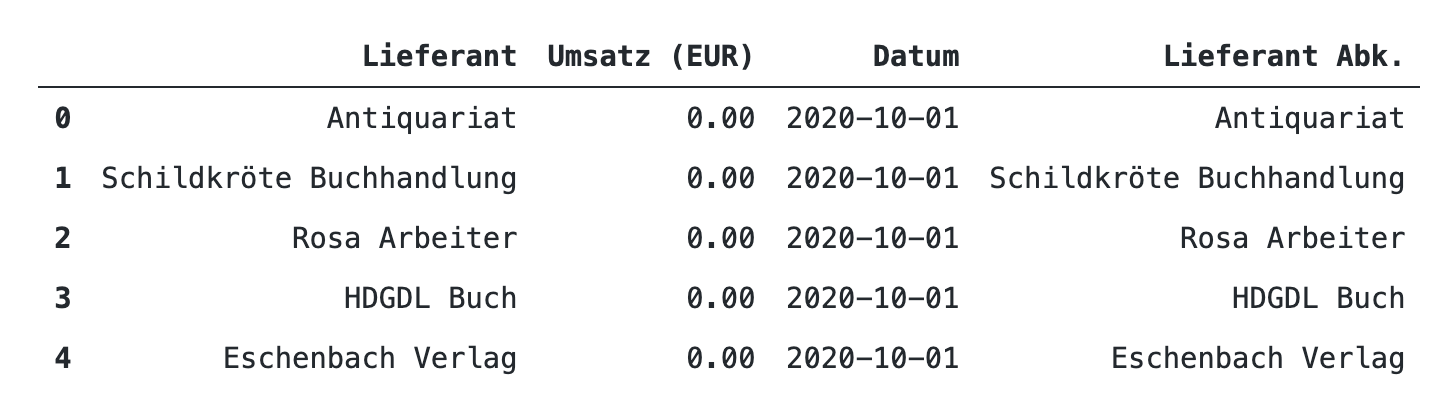
\includegraphics[width=7.5cm, height=4.0cm]{dataframe_example}
            \hspace{1cm}
            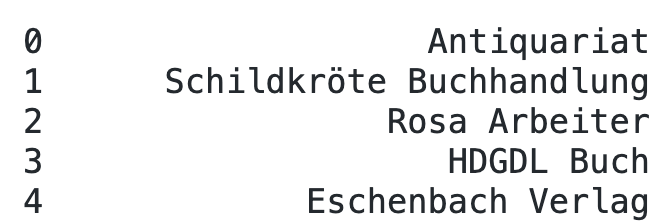
\includegraphics[width=5.0cm, height=4.0cm]{series_example}
            \caption{pandas Dataframe (links) und pandas Series (rechts)}
            \label{fig:pandas Dataframe und pandas Series}
    \end{figure}

    Der Zugriff auf die Series kann über den Spaltenkopf \enquote{Lieferant Abk.} oder indexbasiert erfolgen. 
    Sowohl der Dataframe als auch die Series haben einen Index, über den auf die einzelnen Werte zugegriffen werden kann. 
    
    Auf dem Dataframe, der als sogenannter Container für die Series dient, können verschiedene Operationen der Datenanalyse und 
    -manipulation erfolgen. Ähnlich wie bei Abfragen einer Datenbank lassen sich verschiedene Funktionen wie \texttt{sort()}- oder \texttt{groupby()}
    in Zusammenhang mit Aggregatfunktionen wie \texttt{mean()}, \texttt{median()} oder \texttt{sum()} auf den Series durchführen.
    Auch gibt es eine Vielzahl von Funktionen, um Daten rasch zu explorieren. Zum Beispiel bietet sich in Verbindung mit pandas dazu Jupyter Notebook als
    Entwicklungsumgebung hervorragend an, da in dieser der Code zeilenbasiert ausgeführt werden kann.\footnote{Für das vorliegende Projekt wurden 
    insbesondere Teile der Datenanalyse damit entwickelt und getestet.} Die Werte der Zellen können verschiedene Datentypen
    annehmen. So können beispielsweise die Datumswerte der Spalte \enquote{Datum} in Datetime-Objects umgewandelt werden.

    %In Verbindung mit pandas ist Python neben \textsf{R} im wissenschaftlichen Kontext für Data-Science-Projekte deshalb sehr beliebt.
    
    Es gibt eine Vielzahl an Bibliotheken für Python, die für die Entwicklung von interaktiven Datenvisualisierungen verfügbar sind. Zu
    nennen wären Bokeh \cite[vgl.][]{van_de_ven_bokeh_2021}, Altair \cite[vgl.][]{altair_altair_2021} und die 
    Graphic Libraries von Plotly \cite[vgl.][]{plotly_plotly_2021}.
    Plotly Express ist eine graphische Bibliothek für Python, \textsf{R} und Javascript. Es ist eine Weiterentwicklung (Wrapper) der Bibliothek Plotly Graph Objects. 
    Plotly Express besitzt eine einfachere Syntax bei fast annäherender Feature-Gleichheit mit Plotly Graph Objects \cite[][]{plotly_plotly_2021}.
    So können mit wenigen Zeilen Python-Code interaktive Grafiken erzeugt werden. 
    An interaktiven Basisfunktionalitäten bietet Plotly Express Hover-Informationen der Datenpunkte, Zoom-In und Zoom-Out-Möglichkeiten oder
    das Aus- und Abwählen von Balken oder Linien in den entsprechenden Diagrammen. Plotly Express kann pandas Dataframes 
    oder pandas Series als Datenobjekte erwarten und verarbeiten. Dabei können die Spaltenköpfe die Achsen darstellen 
    und die einzelnen Werte der Spalten die Datenpunkte bilden. Die Rendering-Engine für die Diagramme beruht auf dem JavaScript Framework D3.js. 
    Plotly Express ist frei verfügbar. In Kombination mit der Bibliothek Dash für die Entwicklung von interaktiven Dashboards lässt sich Plotly Express gut anwenden, 
    da beide von der selben Firma entwickelt werden und aufeinander abgestimmt sind.  Für das Projekt wurde sich deswegen für Plotly Express entschieden 
    und dieses hauptsächlich genutzt. 
    
    Mit der Bibliothek Dash wurde das Dashboard realisiert. Dash baut auf den Technologien Flask, plotly.js und React.js auf. Das Framework ermöglicht die Erstellung interaktiver Webapplikationen 
    oder \enquote{Analytical Applications} in Python ohne hierfür mit Javascript programmieren zu müssen \cite[vgl.][]{plotly_dash_2021}.
    Es gibt verschiedene Dash-Komponenten, die unterschiedliche Funktionen erfüllen. \texttt{Dash\_html\_components} stellen Klassen für alle HTML-Elemente bereit.
    Die Schlüsselwortargumente dieser Klasse beschreiben HTML-Attribute wie style, className und id \cite[vgl.][]{plotly_dash_2021-2}. 
    Andere Komponenten sind \texttt{dash\_core\_components} oder \texttt{dash\_dependencies} \cite[vgl.][]{plotly_dash_2021-1}.
    \footnote{Die beiden Module \texttt{dash\_html\_components} und \texttt{dash\_core\_components} werden nach Python-Konventionen als \texttt{html} für die \texttt{dash\_html\_components} und als \texttt{dcc} für die \texttt{dash\_core\_components} bezeichnet und importiert.}
    Während die \texttt{dash\_core\_components}
    Steuerelemente und Graphen erzeugen, regeln die \texttt{dash\_dependencies} über Callback-Dekorator-Funktionen die Interaktion zwischen den einzelnen Komponenten.
    So kann zum Beispiel in der Dash-Webapplikation das Verhalten eines Diagramms von den Werten eines Dropdown-Menü gesteuert werden. 
    % Die zugehörige Callback-Dekorator-Funktion wird in diesem Falle automatisch von Dash aufgerufen, sobald sich der Wert des Dropdown-Menüs ändert. 
    %Dabei bewältigt Dash alle Javascript-Anforderungen im Front- und im Backend \cite[vgl.][]{plotly_dash_2021-3}.
    \texttt{Dash\_bootstrap\_components} ist eine weitere Bibliothek, die zum Einsatz in diesem Projekt kommt. Sie unterstützt die grafische Umsetzung
    des Dashboardes \cite[vgl.][]{faculty_dash_2021}.

    Die \autoref{tab:Software-Requirements} zeigt einen kurzen Überblick über die Versionsnummern der genutzten Programmiersprache und der hauptsächlich 
    genutzten Bibliotheken sowie deren Open-Source Lizenzen.
    
    \begingroup
        \setlength{\tabcolsep}{4pt} % Default value: 6pt
        \renewcommand{\arraystretch}{1.5}
        %\resizebox{\textwidth}{!}{
        \begin{table}[H]
            \centering
            \begin{adjustbox}{max width=\textwidth}
            \Huge
            \begin{tabular}{lccl}
              %\begin{tabular}{p{3cm}p{5cm}p{1cm}p{1.5cm}p{2cm}p{4cm}}
               \toprule
               \textbf{Name}             &{Version}    &\textbf{Lizenz}                        & \textbf{Webseite}\\
               \midrule     
                    Python               &3.7.9         &Open Source (PSF)                     & \url{https://docs.python.org/3.7/}\\
                    pandas               &1.1.5         &3-Clause-BSD-License                  & \url{https://pandas.pydata.org/pandas-docs/version/1.1.5/}\\
                    Plotly               &4.14.1       &MIT-License                           & \url{https://plotly.com/python/}\\
                    Dash                 &1.18.1        &MIT-License                           & \url{https://dash.plotly.com/}\\


                \bottomrule
            \end{tabular}
            \end{adjustbox}
            \caption
            \label{tab:Software-Requirements}
            }
             \end{table}
        \endgroup
    

    \subsection{Systemarchitektur}
    
    Das System teilt sich in drei Teilsysteme auf, die im \autoref{chap:five_one_three} näher beschrieben sind und mit Beispielen erläutert werden. 
    %Teilsystem 4 besteht dahingegen wieder aus objekt-orientierter Programmierung. Genutzt wird hier eine Library, die OOP vorgibt. 
    In der folgenden \autoref{fig:Systemarchitektur} wird die Systemarchitektur des Projektes gezeigt.
    %\footnote{Die schwarzen Pfeile zeigen vereinfacht den Datenfluss an, während der rote Pfeil die Richtung der Methodenaufrufe / Initialisierung der Objelte angibt.}

    \begin{figure}[H]
        \centering
            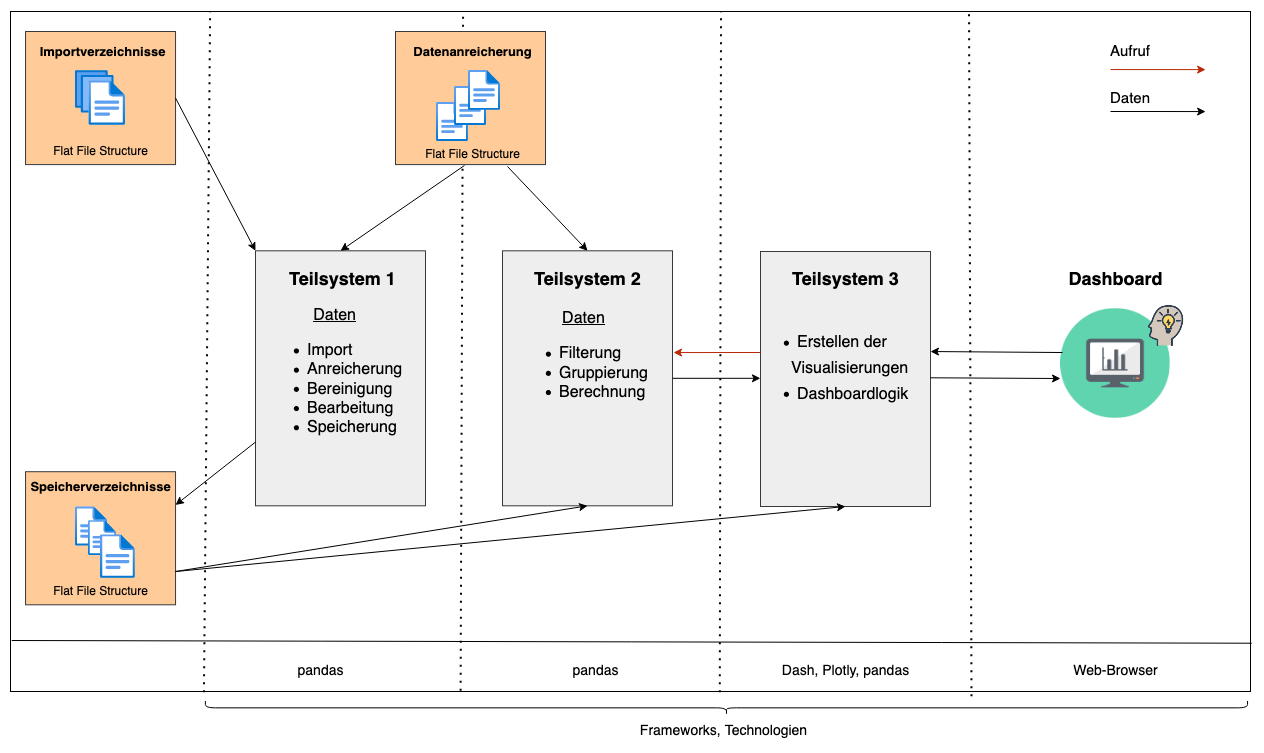
\includegraphics[width=15cm, height=10cm]{Systemarchitektur}
            \caption{Systemarchitektur}
            \label{fig:Systemarchitektur}
    \end{figure}

    Das Hauptziel des Teilsystems 1 ist es, die Daten aus heterogenen Datenquellen in einem einheitlichen Dateiformat zu speichern.
    Das Teilsystem 1 importiert die Daten zunächst aus den Datenquellen und unterwirft sie einem Transformationsprozess, der die Bearbeitung der Daten, die Berechnung
    auf den Daten und die Bereinigung der Daten umfasst. In Abhängigkeit von der Vielschichtigkeit der vorliegenden Daten bedarf dieser Prozess unterschiedlich vieler Transformationsschritte.  
    %Das Teilsystem 1 funktioniert zudem autonom vom Teilsystem 2 und Teilsystem 3. 
    Anschließend werden die in einem einheitlichen Format vorliegenden Daten durch das Teilsystem 2 
    für die Anzeige im Dashboard vorbereitet, indem das Teilsystem 2 mit der Python-Bibliothek pandas die Daten vorfiltert und Berechnungen auf den Daten ausführt. 
    Zudem wird auch noch eine Datenanreicherung vollzogen. Teilsystem 3 ist für das Layout des Dashboards, die Erstellung der Diagramme, die Anordnung der Diagramme im Dashboard und 
    die Bereitstellung von Interaktionen auf dem Dashboard verantwortlich. Die Daten aus dem Teilsystem 2 werden dem Teilsystem 3 übergeben,
    indem das Teilsystem 3 die Filterungen und Berechnungen des Teilsystems 2 aufruft. Teilsystem 3 sorgt für die Übergabe der Daten an das Dashboard zu dessen Anzeigezeit.
    
    Teilsystem 1 und Teilsystem 2 wurden objektorientiert programmiert, da hier der Anspruch bestand, den Programmcode
    für verschiedene Daten wiederzuverwenden. Teilsystem 3 besteht vorerst nur aus Funktionen, die die Anzeige im Frontend ermöglichen.
    \autoref{tab:Teilsysteme} zeigt die drei Teilsysteme mit einer Kurzbeschreibung der Hauptaufgabe.

       \begingroup
            \setlength{\tabcolsep}{4pt} % Default value: 6pt
            \renewcommand{\arraystretch}{1.5}
            %\resizebox{\textwidth}{!}{
            \begin{table}[H]
                \centering
                \begin{adjustbox}{max width=\textwidth}
                \LARGE
                \begin{tabular}{cll}
                  %\begin{tabular}{p{3cm}p{5cm}p{1cm}p{1.5cm}p{2cm}p{4cm}}
                   \toprule
                   \textbf{Teilsystem}             & Name   &{Hauptaufgabe} \\
                   \midrule     
                            1                      &Import  &Import und erste Bereinigung der Daten aus heterogenen Datenquellen.\\
                            2                      &Datenbearbeitung     &Aufbereitung der Daten für die graphische Darstellung im Dashboard.\\
                            3                      &Darstellung          &Umwandlung der Daten in Datenvisualisierungen und Implementierung der Dashboard-Logik.\\
                        %   4                      &Standardbericht      &Export ausgewählter Datenvisualisierungen und Darstellung in Berichtsform.\\

                    \bottomrule
                \end{tabular}
                \end{adjustbox}
                \caption
                \label{tab:Teilsysteme}
                }
                 \end{table}
            \endgroup

    \subsection{Teilsysteme}
    \label{chap:five_one_three}
    
    \clearpage
    \textit{Teilsystem 1 Import}\\
    \begin{figure}[H]
        \centering
            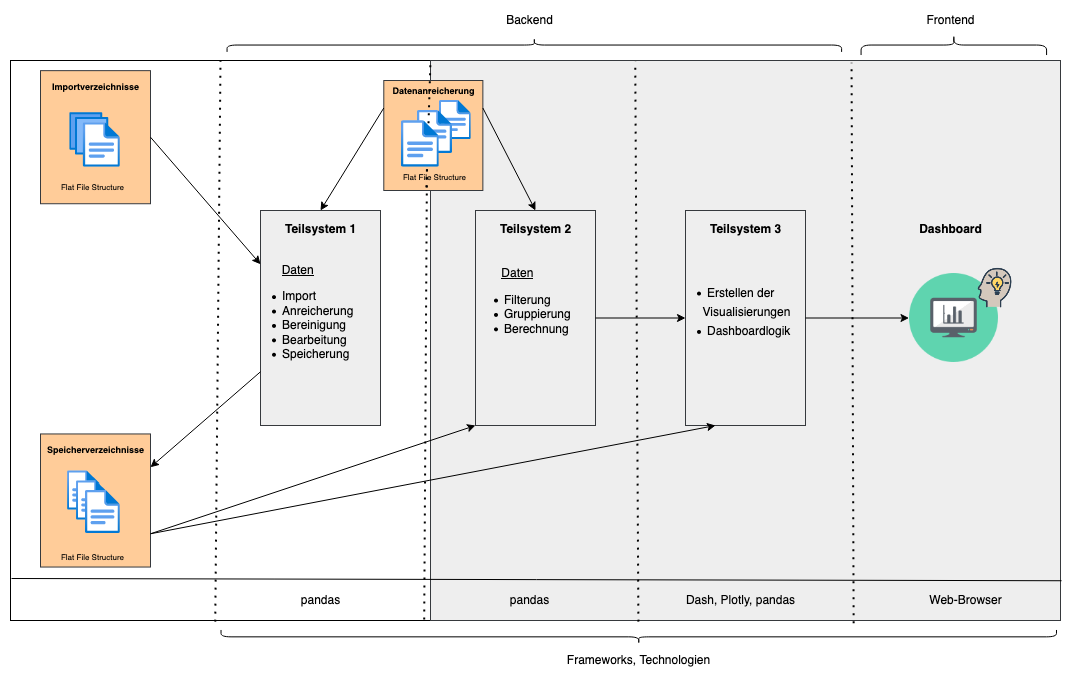
\includegraphics[width=15cm, height=10cm]{Systemarchitektur_Ts1}
            \caption{Systemarchitektur Teilsystem 1}
            \label{fig:Systemarchitektur Teilsystem 1}
    \end{figure}


    Das \textit{Teilsystem 1 Import} ist verantwortlich für den Import der Daten im Rohformat aus vordefinierten Importverzeichnissen 
    in vordefinierte Zielverzeichnisse. Das Layout der Importverzeichnisse ist eine Struktur, die für alle Daten, die importiert werden sollen,
    jeweils einen lokalen Ordner vorsieht. So zum Beisiel gibt es jeweils einzelne Ordner für bibliotheksspezifische Daten wie die Budget- und Umsatzdaten.
    Da anhand der Dateinamen nicht unterschieden werden kann, um welche Daten es sich handelt, wurde diese Struktur eingeführt. 
    \footnote{Der Dateiname, der semantisch einem Datumsformat entspricht, wird als Zusatzinformation bei fast allen Daten mit abgespeichert.
    Anhand dieser Information werden im Teilsystem 2 mitunter die Daten gefiltert.} 
    Da es sich um Daten aus heterogenen Datenquellen handelt, unterscheiden sich die Daten durchaus in der Datenstruktur und im Dateiformat. 
    Das Teilsystem 1 unterstützt bereits den Import der Daten in Formaten wie txt, tsv, xlsx und xls. Diese Formate werden im Teilsystem 1 festgelegt
    und können noch um andere erweitert werden.
    
    Das Ziel des Teilsystems 1 ist einerseits die Daten automatisch ohne Informationsverlust zu importieren 
    und andererseits diese für die weitere Analyse mit notwendigen Daten wie zum Beispiel mit den Daten 
    der \textit{\acrshort{RVK}}-Fachsystematiken anzureichern.\footnote{Das Beispiel wird weiter unten noch ausführlich erläutert.}
    Ferner werden erste Bereinigungen der Daten wie zum Beispiel das Entfernen unnötiger Zeichen durchgeführt. Die Daten werden zum Abschluss im csv-Format abgespeichert. 
    Dabei werden die Daten ebenfalls in der Zeichenkodierung utf-8 gespeichert, um eine syntaktische Homogenität zu gewährleisten. Das Layout der Speicherverzeichnisse
    entspricht dem Layout der Importverzeichnisse. Die Daten liegen in diesen Ordnern jeweils in einer Datei vor, die mit jedem Importprozess um die zu importierenden Daten wächst.

    Mit dem Teilsystem 1 soll eine einheitliche Datengrundlage für die spätere Bearbeitung und Darstellung der Daten garantiert werden. Für das csv-Format wurde sich aufgrund seiner flachen und einfachen Struktur, der guten Lesbarkeit
    und seiner weiten Verbreitung entschieden. Zu vergleichen wäre die Organisation der Speicherung mit einem Data Lake, nur dass hier die Daten in nur einem Dateiformat vorliegen und schon Transformationsprozessen unterzogen worden sind.
    % Die Daten werden jeweils in ein pandas Dataframe geladen. Das Dataframe wird dann verschiedentlich bearbeitet, bevor es zum Schluss als csv-Datei in dem jeweiligen
    % Zielverzeichnis abgespeichert wird.
    
    Das \textit{Teilsystem 1 Import} besteht aus vier Klassen. Die \autoref{fig:classes import} zeigt die einzelnen Klassen mit ihren Methoden.
    Die Klassen im \textit{Teilsystem 1 Import} sind auf die Daten aus fremden Quellen zugeschnitten
    (Budget, Umsatz, Neuerwerbungslisten und Ausleihe (Anwendungsfälle 2, 4, 5 und 6)). Dennoch werden mit mit ihnen auch die bibliotheksinternen Daten
    wie Lesesaalnutzung (Anwendungsfall 3) bearbeitet. 
    \begin{figure}[H]
        \centering
            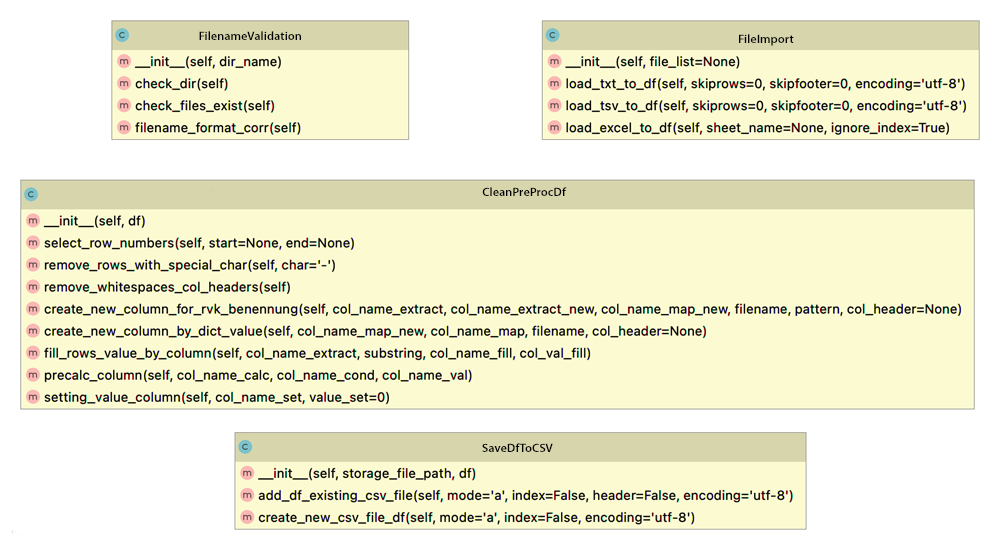
\includegraphics[width=15cm, height=12cm]{data_import_class1}
            \caption{Klassendiagramm - Teilsystem 1 Import}
            \label{fig:classes import}
    \end{figure}

    Instantiiert werden die einzelnen Klassen für die jeweiligen konkreten bibliothekarischen Daten in Python-Skripten. 
    So gibt es Skripte für Budget, Umsatz, Ausleihe und Bestand/Neuerwerbungen. Diese verwenden für die Daten passende Methoden
    aus den Klassen \texttt{FileImport} oder \texttt{CleanPreProcDf}.
    Den Ablauf des Teilsystems zeigt schematisch die \autoref{fig:flow import}.

    \begin{figure}[H]
        \centering
            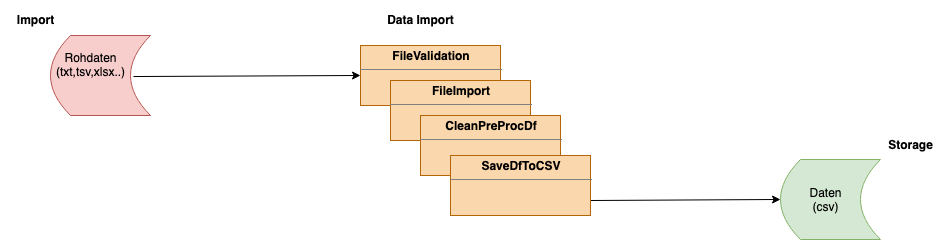
\includegraphics[width=13cm, height=8cm]{flow_imp}
            \caption{Datenfluss - Teilsystem 1 Import}
            \label{fig:flow import}
    \end{figure}

    
    (1) Für den ersten Schritt sind die Klassen \texttt{FilenameValidation} und \texttt{FileImport} verantwortlich.
    Die Dateien werden aus einem lokalen Verzeichnis in ein pandas Dataframe geladen. 
    Dabei wird mit den Methoden der Klasse \texttt{FilenameValidation} überprüft, ob sowohl das Verzeichnis als auch die Dateien existieren.
    Die Pfade für die zu überprüfenden Verzeichnisse werden vom Projektverzeichnis abgeleitet und in der \texttt{configuration.py} festgelegt.
    
    Des Weiteren wird sichergestellt, dass die Dateinamen einem definierten semantischen Format wie dem Datumsformat YYYY\_MM\_DD und 
    einem Dateiformat wie txt-, xlsx- oder tsv-Format entsprechen. Wenn die Daten nicht diesen Vorgaben entsprechen, werden sie nicht in
    das pandas Dataframe geladen. Da die Daten unterschiedlich aufgebaut und in unterschiedlichen Dateiformaten vorliegen, 
    werden beim Laden in den Dataframe jeweils verschiedene Methoden angewandt. Dabei werden spezifische pandas-Funktionen für 
    txt-Dateien oder für xlsx-Dateien eingesetzt, die diese Dateiformate parsen können. 
    Der Parser versucht die Datentypen der Werte in den Spalten aus den vorliegenden Werten der Spalten automatisch abzuleiten. 
    Dabei arbeitet er einen Datentyp nach dem anderen ab. Datentypen in pandas sind zum Beispiel int64, float64 oder objects. 
    Diese entsprechen ähnlichen Python-Typen wie int (int64), float (float64) oder auch Strings (objects). Daneben gibt es noch spezielle pandas Datentypen wie die bereits erwähnten Datetime-Objects, die aber nicht automatisch zugewiesen werden.
    Zunächst versucht pandas die Werte in Integerwerte zu konvertieren. Tritt in diesem Erkennungsprozess ein Fehler auf, 
    wird zum nächsten Datentyp übergegangen. Wenn kein spezifischer Datentyp erkannt wird, werden die Werte in den allgemeinen Datentyp objects konvertiert \cite[vgl.][]{golubin_how_2021}.
    \footnote{Die Erkennung des Datentyps funktioniert durchaus auch für andere Dateiformate und nicht nur für csv-Formate. Das gelang für das vorliegende Projekt gut, sodass
    bei diesem Prozess nicht manuell eingegriffen wurde.}
    
    Beim Ladeprozess der Dateien in den pandas Dataframe wird mit den Methoden \texttt{load\_txt\_to\_df()} oder \texttt{load\_tsv\_to\_df()} 
    der Klasse \texttt{FileImport} der Dateiname von der Datei extrahiert und in einer neu geschaffenen Spalte des Dataframes im Datumsformat YYYY-DD-MM gespeichert.
    Anhand der Werte dieser Spalte werden später verschiedene Datenanalysen und Datenvisualisierungen vollzogen.\footnote{Dieses Verfahren wird bei den Daten ausgeführt, die einer zusätzlichen Datumsspalte bedürfen.} 
    Verantwortlich für die Extrahierung des Dateinamens ist die in \texttt{utils.py} ausgelagerte Funktion \texttt{date\_from\_filename()},
    die den Dateinamen als Argument entgegennimmt.\footnote{In der Datei \texttt{utils.py} sind noch andere Funktionen als stand-alone-functions für den Datenimport und Datenbearbeitung gruppiert,
    da diese das Objekt \texttt{self} nicht verändern. Zu finden ist die Datei im Projekt in dem Verzeichnis \texttt{src}.} 
    
    (2) Das geladene pandas Dataframe wird im zweiten Schritt durch die Klasse \texttt{CleanPreProcDf} aufgenommen und durch verschiedene Methoden dieser Klasse
    manipuliert. Beispielhaft ist hier die Methode \texttt{create\_new\_column\_for\_rvk\_benennung()} zu nennen, die aus einer Spalte einen Substring unter
    zu hilfenahme eines regulären Ausdruckes extrahiert, diesen in eine neue Spalte schreibt und ihn um zusätzliche Informationen anreichert. 
    Diese Methode wird sowohl bei den Neuerwerbungs-/Bestandsdaten als auch bei den Ausleihdaten zweimal angewendet, um die \textit{\acrshort{RVK}}-Fachsystematiken von den
    Titelsignaturen zu extrahieren und durch die \textit{\acrshort{RVK}}-Benennungen anzureichern. 
    Zunächst werden die Untergruppen der Fachsystematiken aus der Signatur extrahiert, in einer neuen Spalte gespeichert und um die entsprechenden Benennungen der Untergruppen der 
    \textit{\acrshort{RVK}} angereichert. 
    Danach werden die Fachsystematiken aus den Untergruppen extrahiert und ebenfalls um die entsprechenden Bennungen angereichert.
    Mit der \autoref{fig:extr Fachsystematik} lässt sich beispielhaft dieser Prozess an der Signatur \enquote{CP 2000 zit 2018} nachvollziehen.
    \begin{figure}[H]
        \centering
            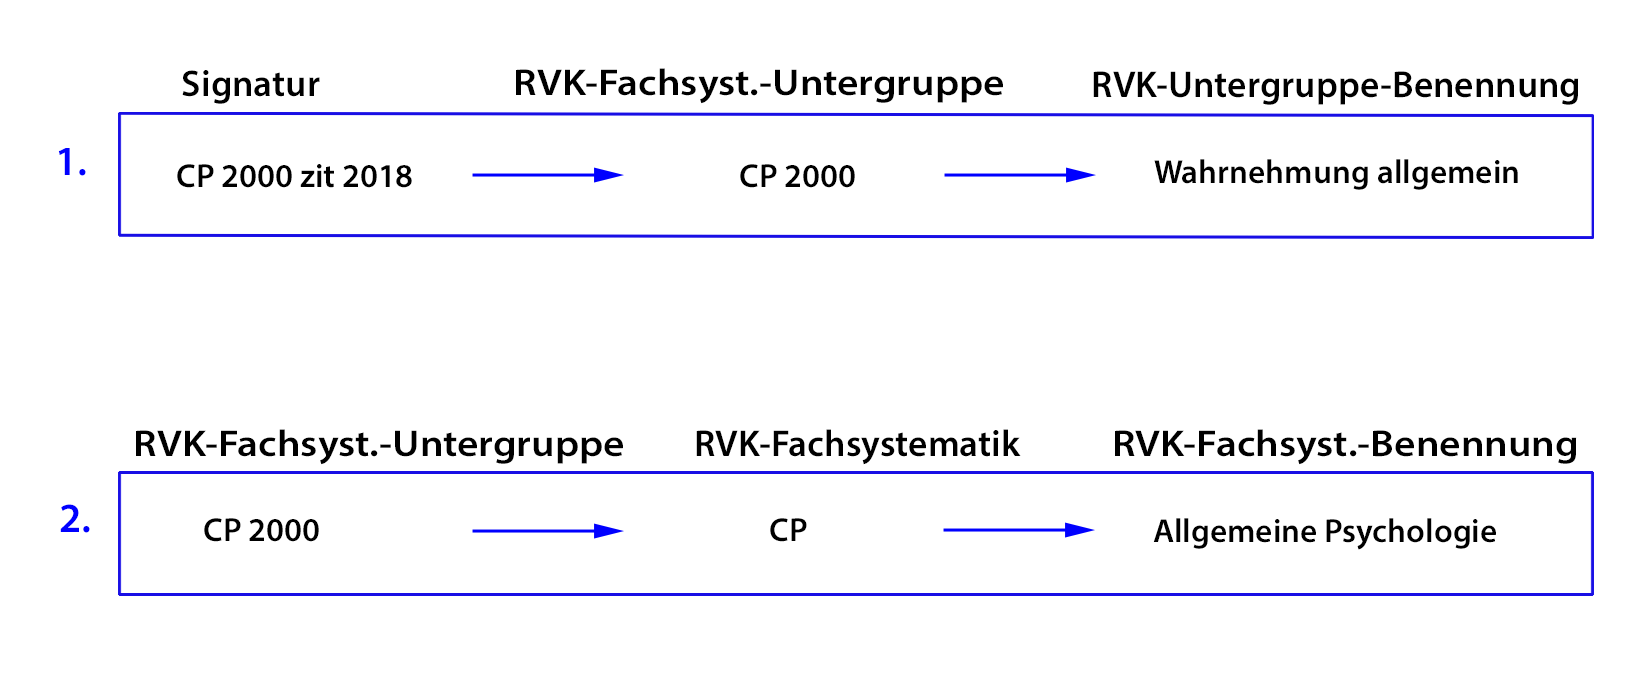
\includegraphics[width=14cm, height=6cm]{signatur_extr}
            \caption{Beispiel Extraktion Fachsystematik}
            \label{fig:extr Fachsystematik}
    \end{figure}

    Zu dem Zweck der Extraktion liegt eine csv-Datei der \textit{\acrshort{RVK}} zu Grunde, die mit einem Python-Skript\footnote{Das Skript liegt im Projektverzeichnis
    unter \texttt{src}} aus einer \textit{\acrshort{RVK}}-XML-Datei entstanden ist.
    Diese XML-Datei kann von der \textit{\acrshort{RVK}}-Homepage bezogen werden und wird ungefähr vierteljährlich aktualisiert \cite[vgl.][]{rvk_rvk_2021}.
    In dieser liegen die Fachsystematiken und die Untergruppen mit ihren Benennungen vor.\footnote{Manuell ergänzt wurde diese noch um selbstgeschaffene Fachsystematiken der Institutsbibliothek.}
    Diese csv-Datei wird bei jedem Aufruf der Methode mit den Werten der neu entstanden Spalte gemappt. Die Benennungen werden ebenfalls in je einer Spalte gespeichert.
    Ziel ist es, die Neuerwerbung- und Bestandsdaten später nach den \textit{\acrshort{RVK}}-Fachsystematiken und deren Untergruppen auszuwerten.
    
    
    Bei den Umsatz- und Budgetdaten entstehen ebenfalls neue Spalten. In Bezug auf die Darstellung der Daten im Dashboard werden
    hier die Namen der Lieferanten und Kostenstellen in lesbarer Form in einer neuen Spalte gespeichert. Für die lesbaren Namen wird ebenfalls auf csv-Dateien zurückgegriffen, in denen die Informationen abgespeichert sind.
    Des Weiteren gibt es in der Klasse \texttt{CleanPreProcDf} Methoden, die für die Entfernung von Zeilen mit bestimmten syntaktischen Zeichen wie Bindestrichen 
    verantwortlich sind oder die eine Vielzahl unnötiger Leerzeichen in Spaltenköpfen löschen  und durch ein Leerzeichen ersetzt.
    Ferner wird eine Berechnung durch die Methode \texttt{precalc\_column()} auf den Ausleihdaten ausgeführt.
    \footnote{Im Arbeitsprozess der Medienerschließung validiert die Bibliothek die RFID-Etiketten der Medien durch einmalige Ausleihe der Medien am Selbstverbucher.
    Deswegen wird die Anzahl der Ausleihe pro Medium um eins reduziert, wenn sie ein oder mehrmals ausgeliehen wurden.}
     
    (3) Nach dem Transformationsprozess wird das veränderte pandas Dataframe in einer csv-Datei in einem vorher definierten Speicherordner gespeichert. 
    Verantwortlich ist dabei die Klasse \texttt{SaveDFToCSV} mit den zwei Methoden \texttt{add\_df\_existing\_csv\_file()} und 
    \texttt{create\_new\_csv\_file\_df()}. 
    Es wird durch diese Methoden entweder eine neue csv-Datei mit dem Dataframe erstellt oder der Dataframe wird an eine bereits vorhandene csv-Datei angehängt.
    \autoref{fig:umsatzuebersicht_txt} zeigt eine Umsatz-Datei, die im txt-Format gespeichert wurde. Die anschließende Transformation durch das Teilsystem 1
    verwandelt die Datei in eine csv-Datei, die in \autoref{fig:umsatzuebersicht_csv} zu sehen ist.

    \begin{figure}[H]
        \centering
            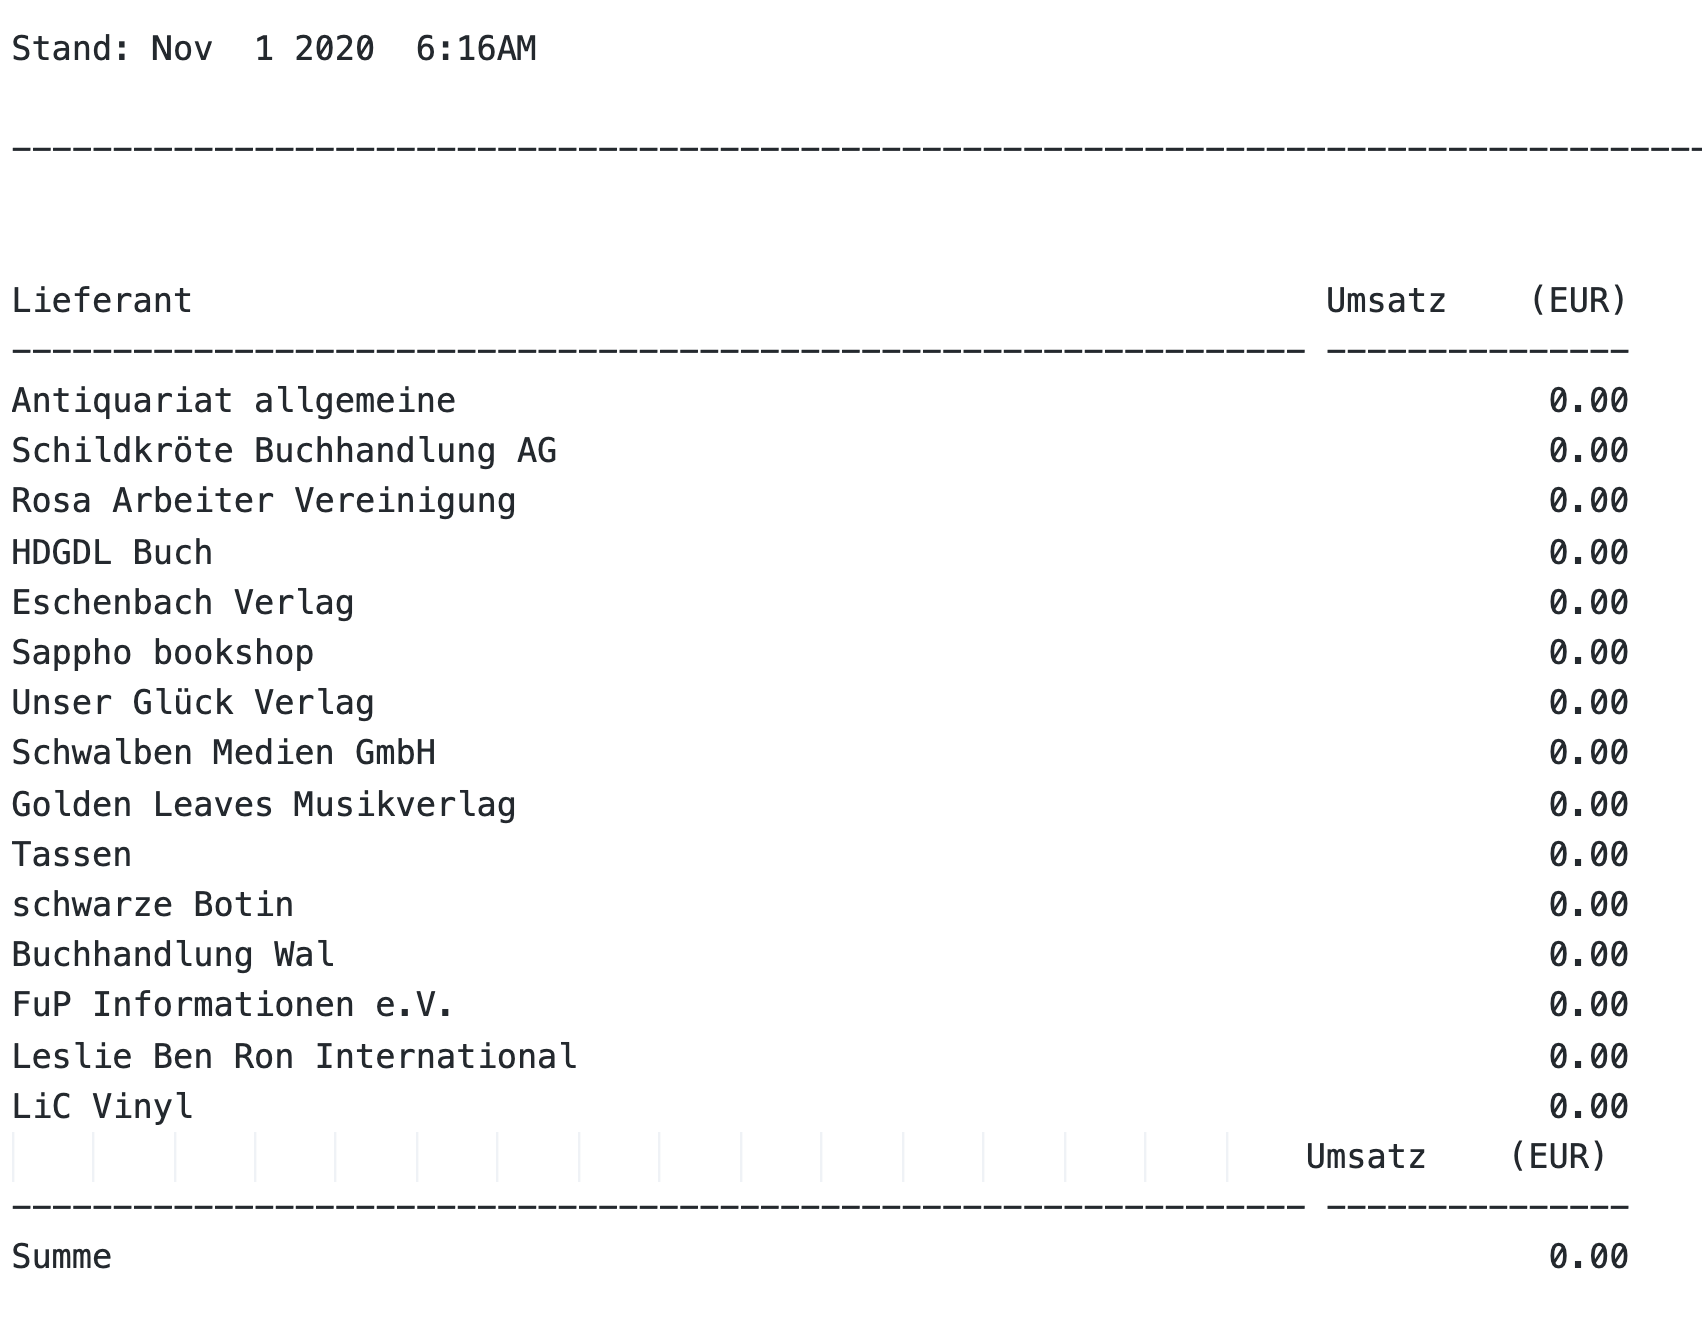
\includegraphics[width=8.5cm, height=8.0cm]{umsatz_mtl}
            %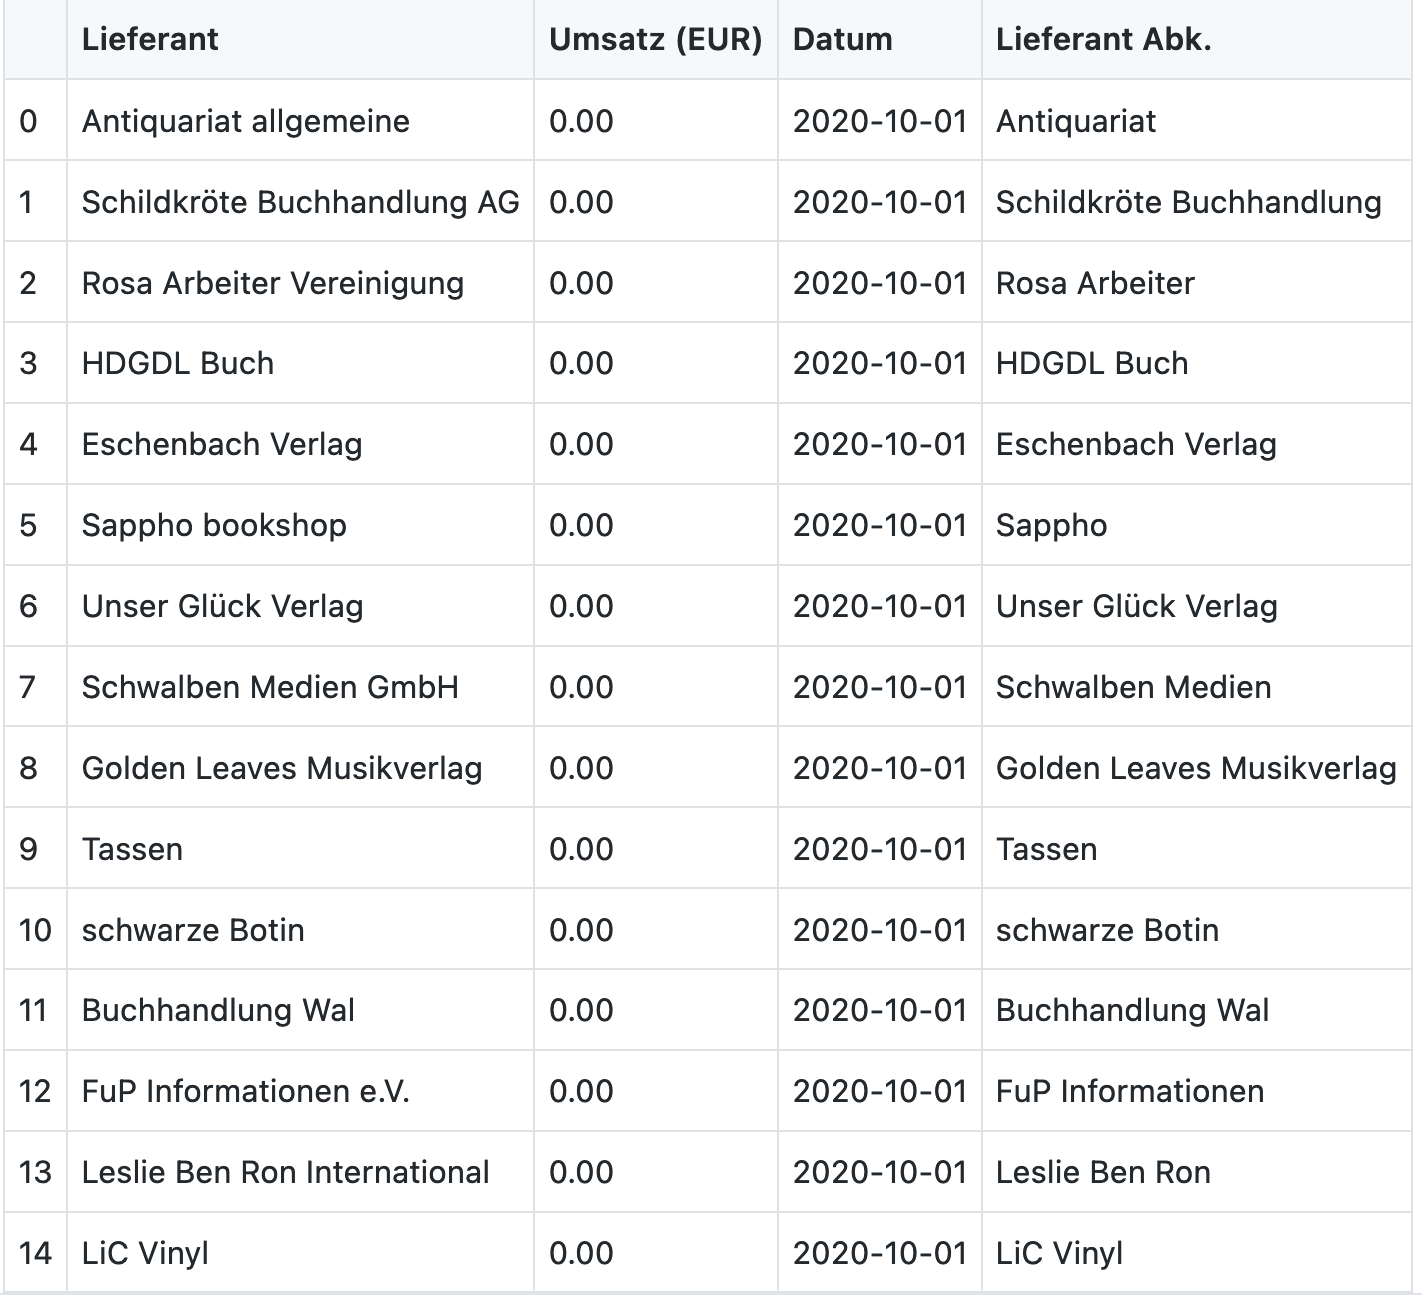
\includegraphics[width=6.5cm, height=7.0cm]{umsatz_csv}
            \caption{Monatliche Umsatzübersicht vor Ablauf Teilsystem 1 Import}
            \label{fig:umsatzuebersicht_txt}
    \end{figure}


    \begin{figure}[H]
        \centering
            %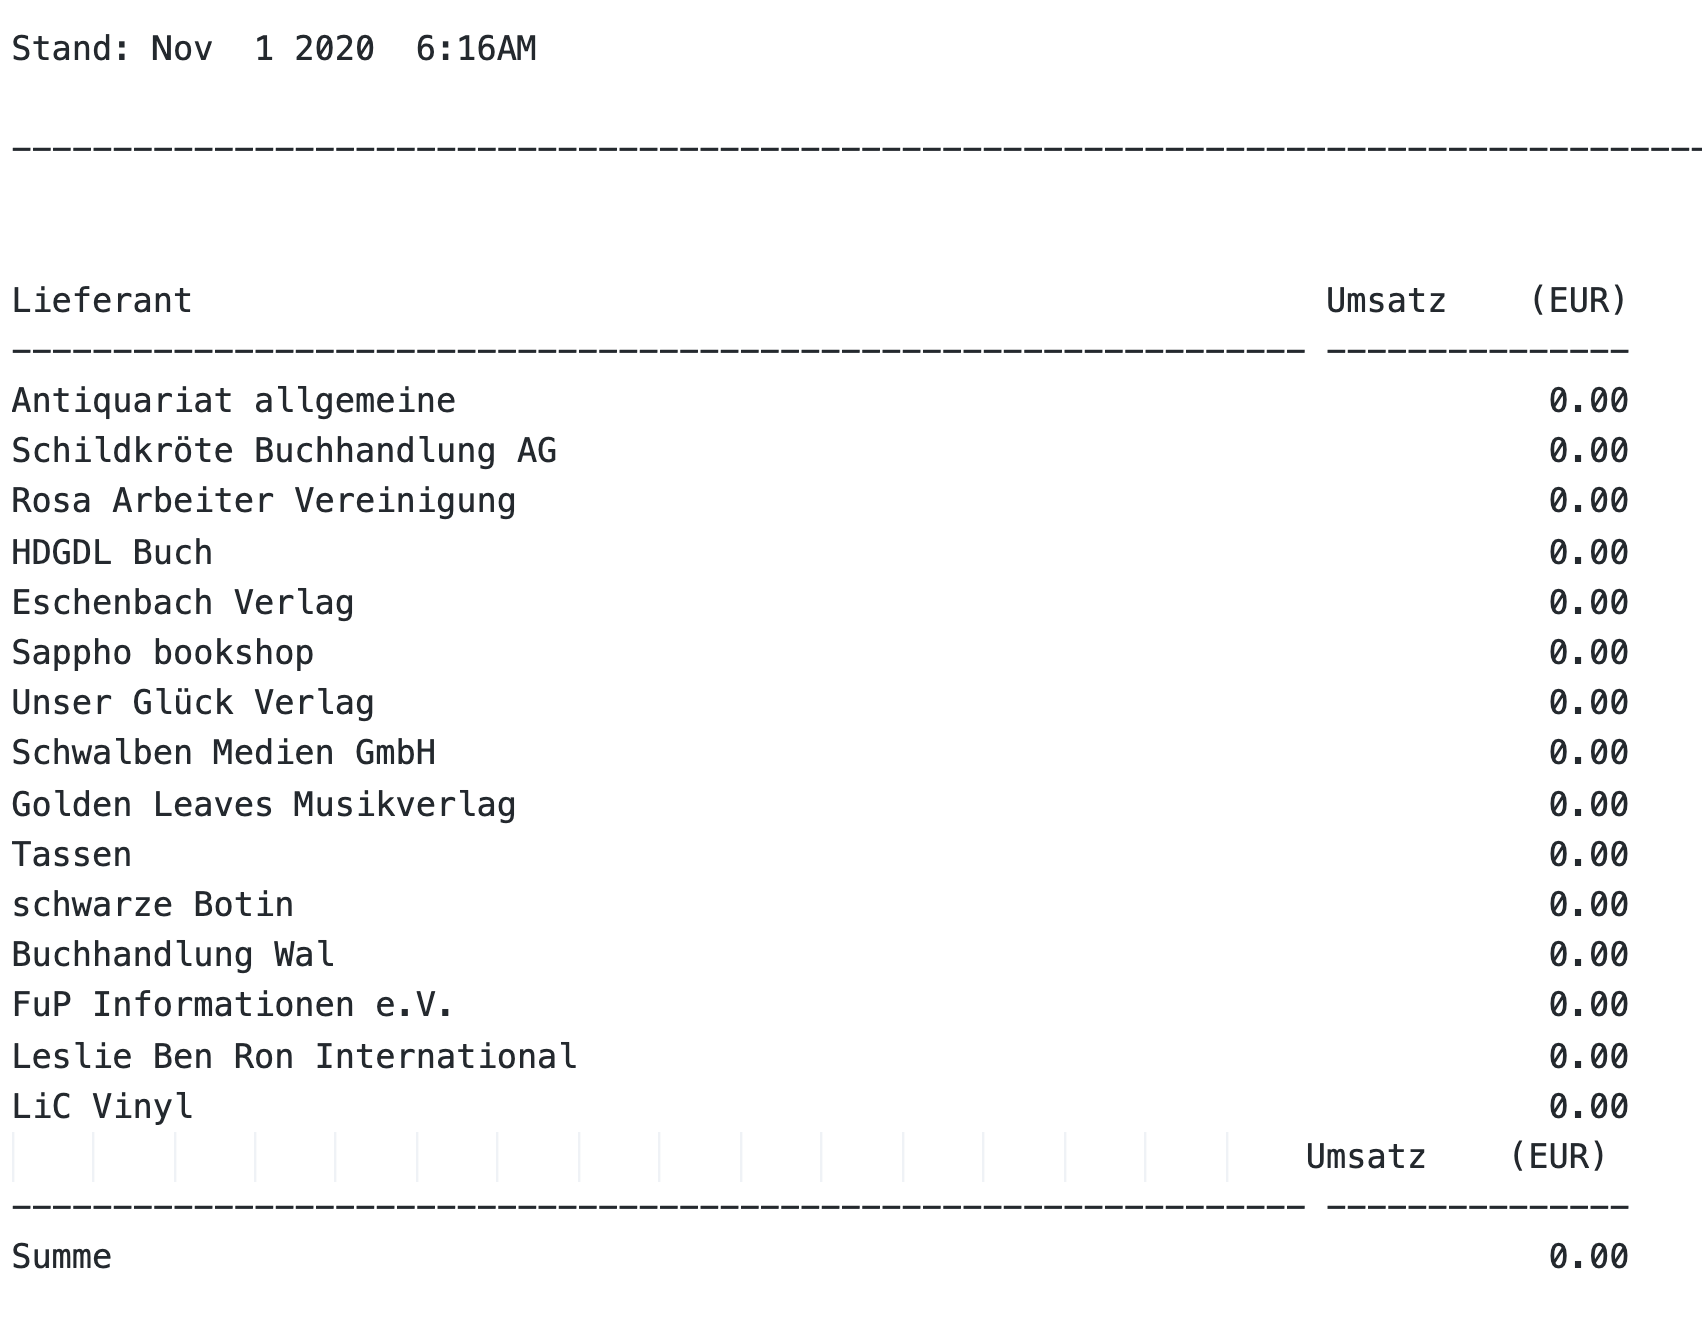
\includegraphics[width=6.5cm, height=7.0cm]{umsatz_mtl}
            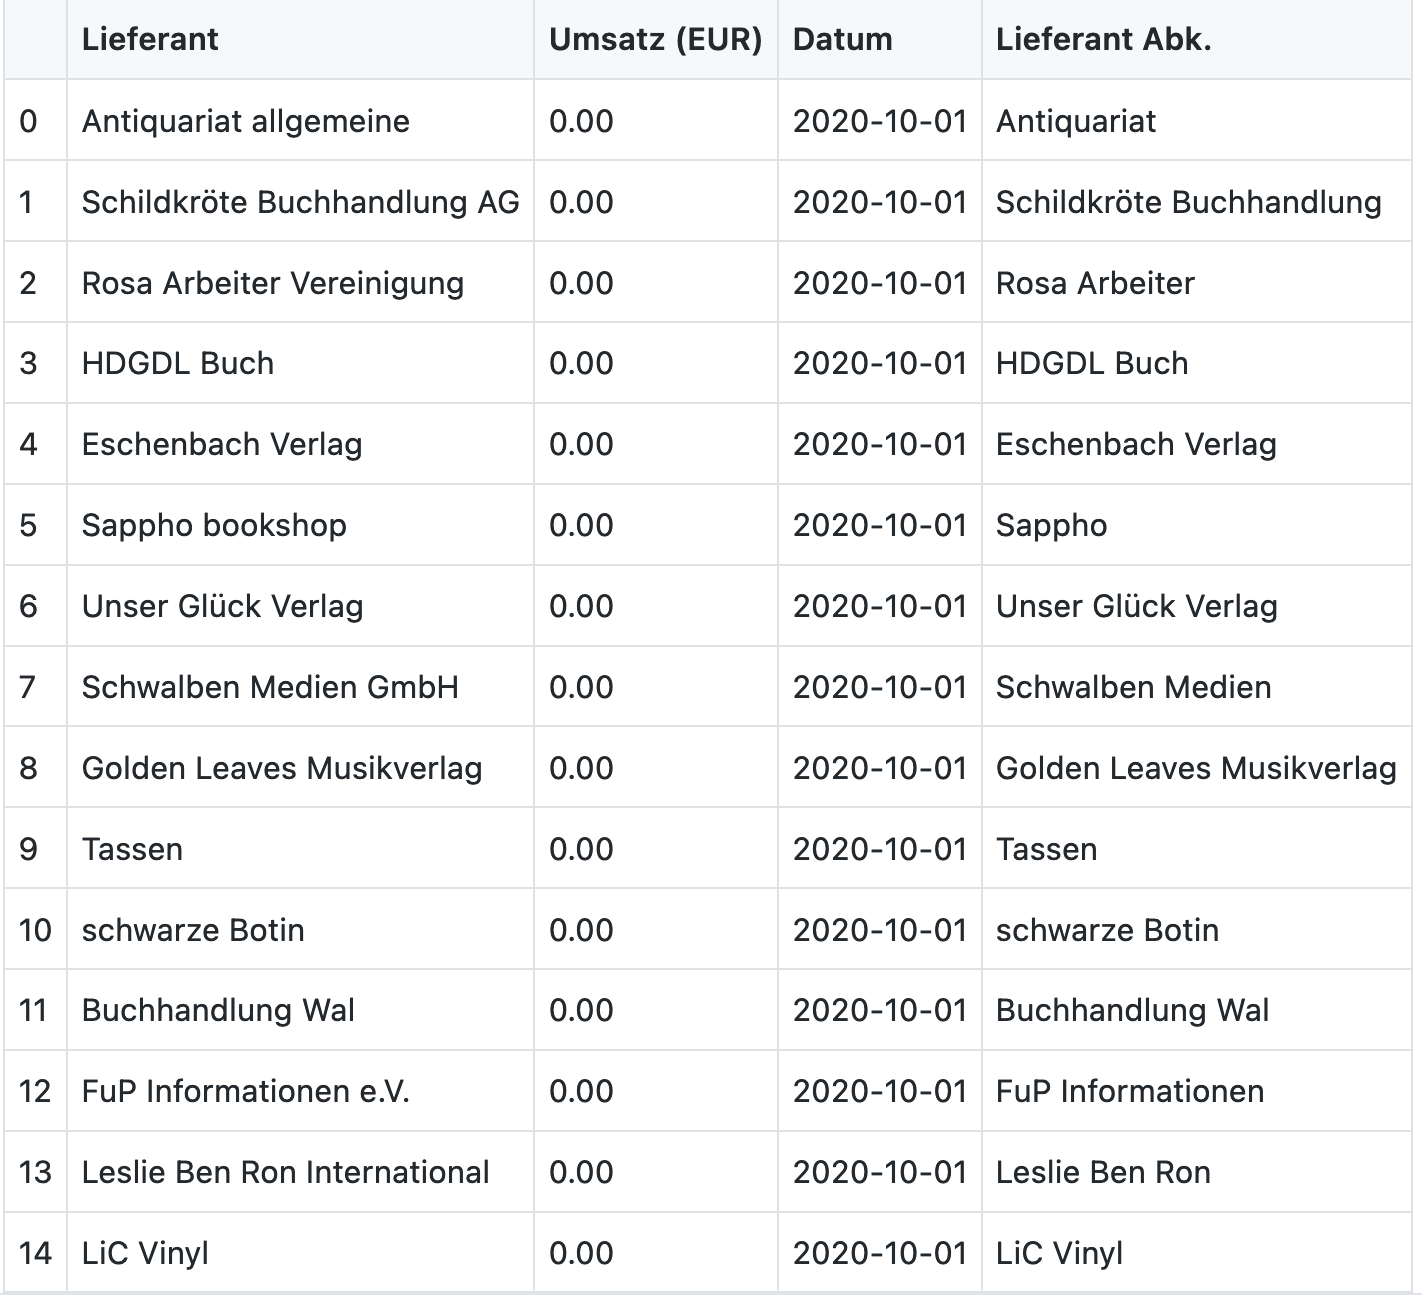
\includegraphics[width=8.5cm, height=8.0cm]{umsatz_csv}
            \caption{Monatliche Umsatzübersicht nach Ablauf Teilsystem 1 Import}
            \label{fig:umsatzuebersicht_csv}
    \end{figure}

    Die Daten liegen nun in den Speicherverzeichnissen vor und können durch das \textit{Teilsystem 2 Datenbearbeitung} 
    weiterbearbeitet werden.
    
    \clearpage
    \noindent
    \textit{Teilsystem 2 Datenbearbeitung}

    \begin{figure}[H]
        \centering
            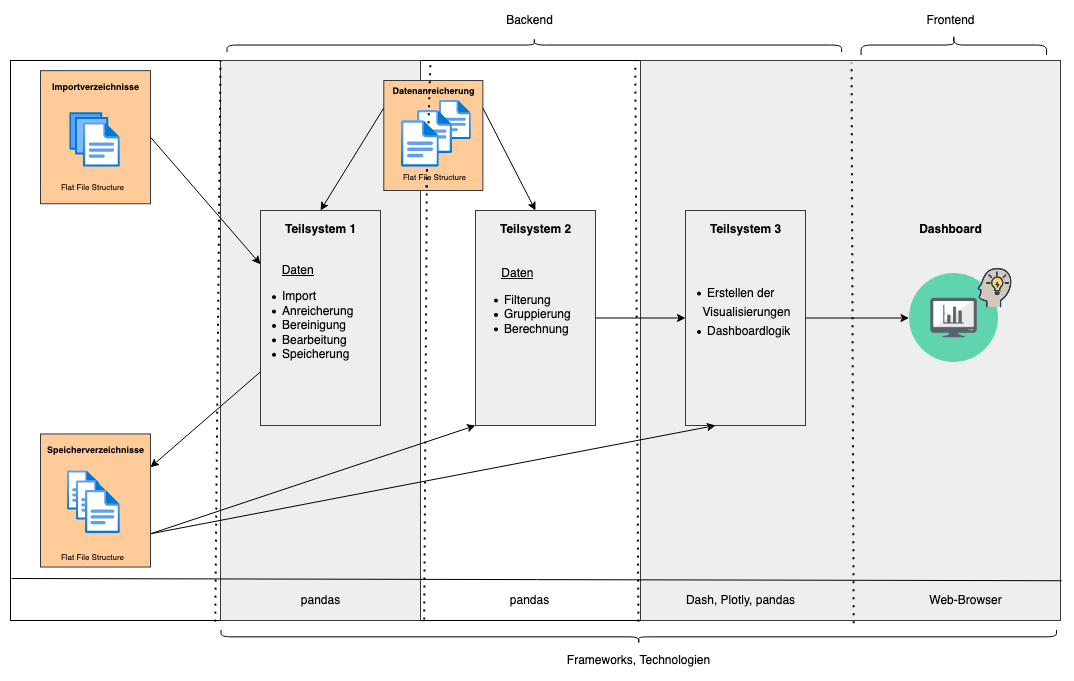
\includegraphics[width=15cm, height=10cm]{Systemarchitektur_Ts2}
            \caption{Systemarchitektur Teilsystem 2}
            \label{fig:Systemarchitektur Teilsystem 2}
    \end{figure}

    Das \textit{Teilsystem 2 Datenbearbeitung} hat das Ziel, die Daten für die Darstellung im Dashboard vorzubereiten. Ein weiterer Zweck dieses
    Teilsystem ist, die Vorbereitung der Daten von der Erstellung der Datenvisualisierungen zu trennen. Ein Grund hierfür
    ist, den Programmcode im Teilsystem 3 nicht mit dem Programmcode der Datenmanipulation zu überfrachten. 
    Deswegen werden in dem Teilsystem Datenbearbeitung Daten mit pandas so bearbeitet, 
    dass entweder nur noch Teilmengen der eigentlichen Daten oder Ergebnisse mathematischer Operationen durch das Teilsystem 3 
    zu Datenvisualisierungen weiterverarbeitet werden müssen. 
    Die Berechnungen des Teilsystems werden zur Laufzeit des Dashboards ausgeführt und somit im Hauptspeicher gehalten.
    Die Vorbereitung der Daten umfasst einzelne Berechnungen 
    wie \texttt{mean()} oder \texttt{sum()}. Ferner werden im Teilsystem 2 die Sortierung, Gruppierung und Filterung der 
    Daten nach bestimmten Aspekten vollzogen, die in den Anwendungsfällen im \autoref{chap:four_one_five} formuliert sind.
    
    Für das \textit{Teilsystem 2 Datenbearbeitung} ist das Modul \texttt{data\_prep} zentral. Die Klassenstruktur dieses Moduls ist eine 
    Basisklasse, von der vier Kindklassen erben. Es gibt Kindklassen für Umsatz- und Budgetdaten, für Bestands- und Neuerwerbungsdaten sowie für die Daten der Ausleihe und 
    der Lesesaalnutzung. Aufgrund der ähnlichen Datenstruktur der Umsatz- und Budgetdaten genügt eine Klasse für beide.
    Der Gesamtbestand und die monatlichen Neuerwerbungen berufen sich auf denselben Datenbestand, sodass hier ebenfalls auf eine Aufteilung auf mehrere Klassen verzichtet wurde.
    Für jede Kindklasse wurden Methoden geschrieben, die auf den spezifischen Bibliotheksdaten verschiedene Manipulationen ausführen.
    Die Ergebnisse werden von jeder Methode zurückgeben. \autoref{fig:classes data_prep} zeigt die Basisklasse und die vier Kindklassen mit ihren Methoden.

    \begin{sidewaysfigure}

    %\begin{figure}[H]
        \centering
            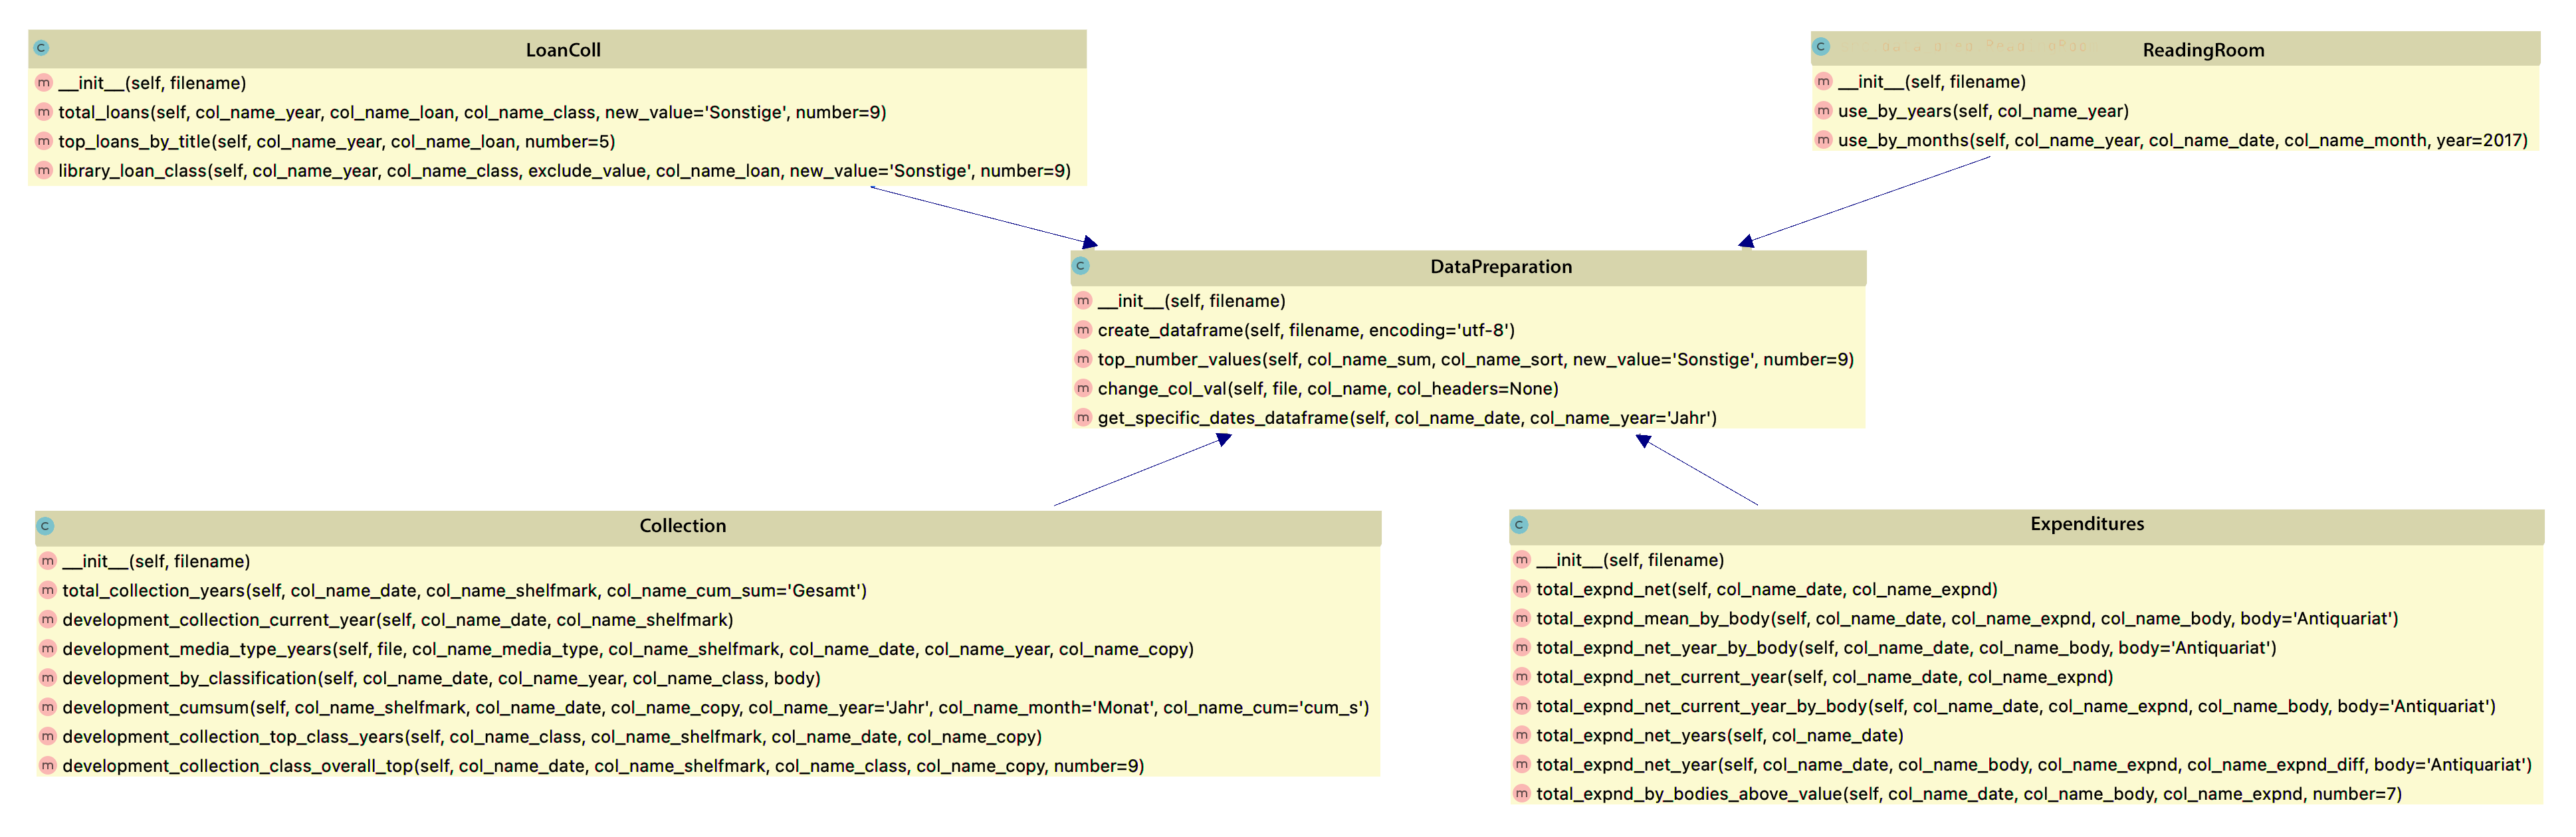
\includegraphics[width=21.5cm, height=12cm]{data_prep_class}
            \caption{Klassendiagramm - Teilsystem 2 Datenbearbeitung}
            \label{fig:classes data_prep}
    \end{sidewaysfigure}
    %\end{figure}

    Der Ablauf innerhalb des Teilsystems besteht aus zwei Schritten.\\
    (1) Das Laden der einzelnen csv-Dateien aus dem Zielverzeichnis in die pandas Dataframes wird durch die Methode \texttt{create\_dataframe()} der Basisklasse geregelt.
    %Es wird noch einmal sichergestellt, dass die Daten in einem Zeichenformat wie utf-8 in das pandas Dataframe geladen werden.
    Beim Aufrufen des Konstruktors beziehungsweise der \texttt{init}-Methode der Klasse wird die Methode \texttt{create\_dataframe()} 
    automatisch mit aufgerufen. In den Kindklassen kann dann ebenfalls das Objekt mit dem pandas Dataframe instantiiert werden, da die Konstruktor-Properties der Basisklasse 
    an die Kindklassen mitvererbt werden. Die Objekte können nach Instantiierung durch die spezifischen Methoden der Kindklassen bearbeitet werden.
    
    (2) Das Ergebnis der Manipulation der pandas Dataframes ist auf die Darstellung der Daten im Dashboard ausgerichtet. Als Input der einzelnen Methoden der
    Kindklassen werden verschiedene Parameter verlangt, mit deren Hilfe der Dataframe entweder manipuliert wird oder auf ihm Berechnungen ausgeführt werden können. 
    Um die Daten für das Teilsystem 3 vorzubereiten, können verschiedene Transformationsschritte auf den Daten innerhalb der Methoden ausgeführt werden. 
    Die Rückgabewerte der Methoden sind veränderte pandas Dataframes, pandas Series oder einzelne Skalare mathematischer Operationen.
    
    % Bei der folgenden Methode interessieren für die Darstellung im Dashboard nur die Umsatz/Budget-Daten für spezifische Datums-Daten. Hintergrund ist der, dass die 
    % monatlichen Umsatz- und Budgetdaten im Jahr akkumuliert werden. Wenn das Budget und der Umsatz nur Jahresweise dargestellt werden sollen, 
    % interessieren dementsprechend nur die Datensätze jeweils vom Dezember beziehungsweise vom aktuellen Monat im Jahr.
    

    % \begin{lstlisting}[language=Python, caption=Python example]
        
    %     def total_expnd_net_years(self, col_name_date):
    %         ...
    %         self._df = self.get_specific_dates_dataframe(col_name_date)
    %         return self._df

    % \end{lstlisting}
    

    % Die Methode \texttt{total\_expnd\_net\_years} der \texttt{Expenditures}-Klasse gibt nach einem Transformationsschritt einen pandas Dataframe zurück.
    % Der Transformationsschritt beinhaltet die Filterung des Dataframes nach spezifischen Werten in der Spalte des übergebenden Spaltennamens.
    % Zu diesem Zweck wird noch die Methode\\
    % \texttt{get\_specific\_dates\_dataframe} aufgerufen. 
    Anhand der folgenden Methode \texttt{total\_expnd\_net\_current\_year()} soll der zweite Schritt verdeutlicht werden.
    Die Methode der \texttt{Expenditures}-Klasse bestimmt im Allgemeinen die Summe von Werten einer Spalte, gefiltert
    nach einem Wert einer anderen Spalte ein und desselben pandas Dataframes. Mit dieser Methode soll so beispielsweise konkret der Gesamtumsatz des 
    laufenden Jahres bestimmt werden.

    \begin{lstlisting}[language=Python, caption=Beispiel Methode Expenditures class]
    def total_expnd_net_current_year(self, col_name_date, col_name_expnd):
        ... 
        date_max = self._df[col_name_date].max()        
        self._df = self._df.set_index(col_name_date)
        self._df = self._df.loc[date_max]

        return self._df[col_name_expnd].sum()  
    \end{lstlisting}

    Als Input erwartet die Methode in der Methodensignatur zwei Spaltennamen als Parameter: den Namen der Datumspalte \texttt{col\_name\_date}, nach der gefiltert wird,
    und den Namen der Umsatz-Spalte \texttt{col\_name\_expnd}, auf der die Berechnung stattfindet. Der Transformationsprozess im Methodenkörper teilt sich in drei Schritte auf. Da die monatlichen Umsatzdaten pro Jahr als 
    akkumulierte Daten vorliegen, interessieren nur die Datensätze mit dem größten Datumswert. Deswegen
    wird nach diesen gefiltert und ein Dataframe von diesen erstellt. Dementsprechend wird mit der pandas-Funktion \texttt{max()} 
    zunächst der maximale Wert in der Datumsspalte bestimmt und der Variable \texttt{date\_max} zugewiesen. Danach wird die Datumsspalte als Index gesetzt. 
    Im dritten Schritt wird der Dataframe mit den Reihen, die der Variable \texttt{date\_max} entsprechen, erstellt. Dies geschieht mit der pandas-Funktion \texttt{.loc}, die
    auf den Index der Reihen des Dataframes zugreift. Zum Schluss wird auf Basis der Umsatz-Spalte des Dataframes die Summe mit der pandas-Funktion \texttt{sum()} berechnet 
    und als Rückgabewert zurückgeliefert. Der Rückgabewert kann nun vom \textit{Teilsystem 3 Darstellung} weiterverarbeitet werden.\\

    \noindent
    \textit{Teilsystem 3 Darstellung}\\

    \begin{figure}[H]
        \centering
            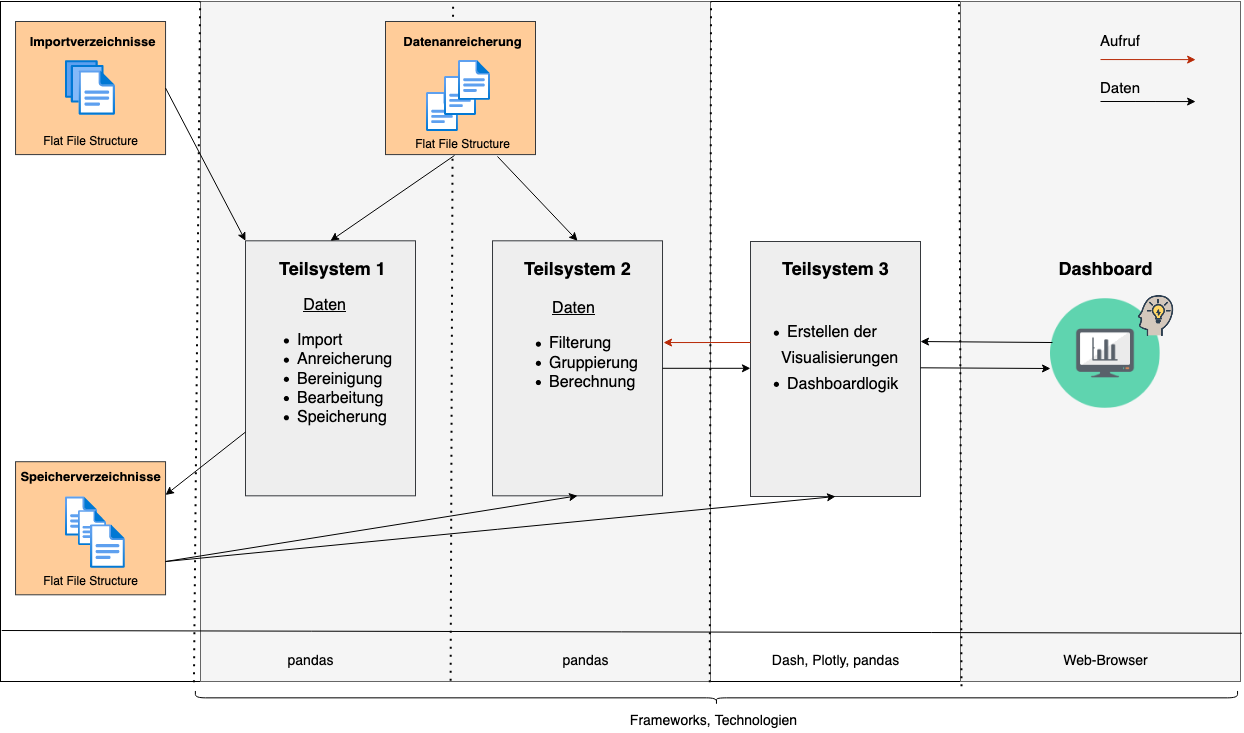
\includegraphics[width=15cm, height=10cm]{Systemarchitektur_Ts3}
            \caption{Systemarchitektur Teilsystem 3}
            \label{fig:Systemarchitektur Teilsystem 3}
    \end{figure}

    Für die Erschaffung des Dashboards mit seinen Datenvisualisierungen und Interaktionen ist das \textit{Teilsystem 3 Darstellung} verantwortlich.
    In ihm werden die Ergebnisse des Teilsystems 2 zu Datenvisualisierungen verarbeitet und die Dashboard-Logik bereitgestellt.
    Die Bibliothek Plotly Express wird für die Datenvisualisierungen und die Bibliothek Dash zur Umsetzung des Dashboards genutzt. 
    Die Übergabe der Daten erfolgt durch den Aufruf der Objekte und der Methoden aus den Kindklassen des \texttt{data\_prep}-Moduls aus dem Teilsystem 2.
    %In ihm werden die Datenvisualisierungen mit den den Ergebnissen aus dem Teilsystem Datenbearbeitung
    %geschaffen. 
    
    Aufgrund der Vielzahl an Datenvisualisierungen wurde sich für das Dashboard gegen eine Single-Page-Lösung entschieden. Deswegen besteht das Dashboard
    aus drei einzelnen Tabs, auf die die einzelnen Datenvisualisierungen aufgeteilt sind. Die Struktur der Dashboard-App entspricht einem Multi-App-Dashboard.
    für dass es verschiedene Möglichkeiten gibt, es zu strukturieren.
    % Aufgrund der vielen Code-Blöcke tendieren Dashboards-Apps, die mit Dash geschrieben wurden zur Unübersichtlichkeit.
    Für das vorliegende Projekt wurde sich für die in 
    \autoref{fig:dash structure} gezeigte Struktur entschieden.

    \begin{figure}[H]
        \centering
            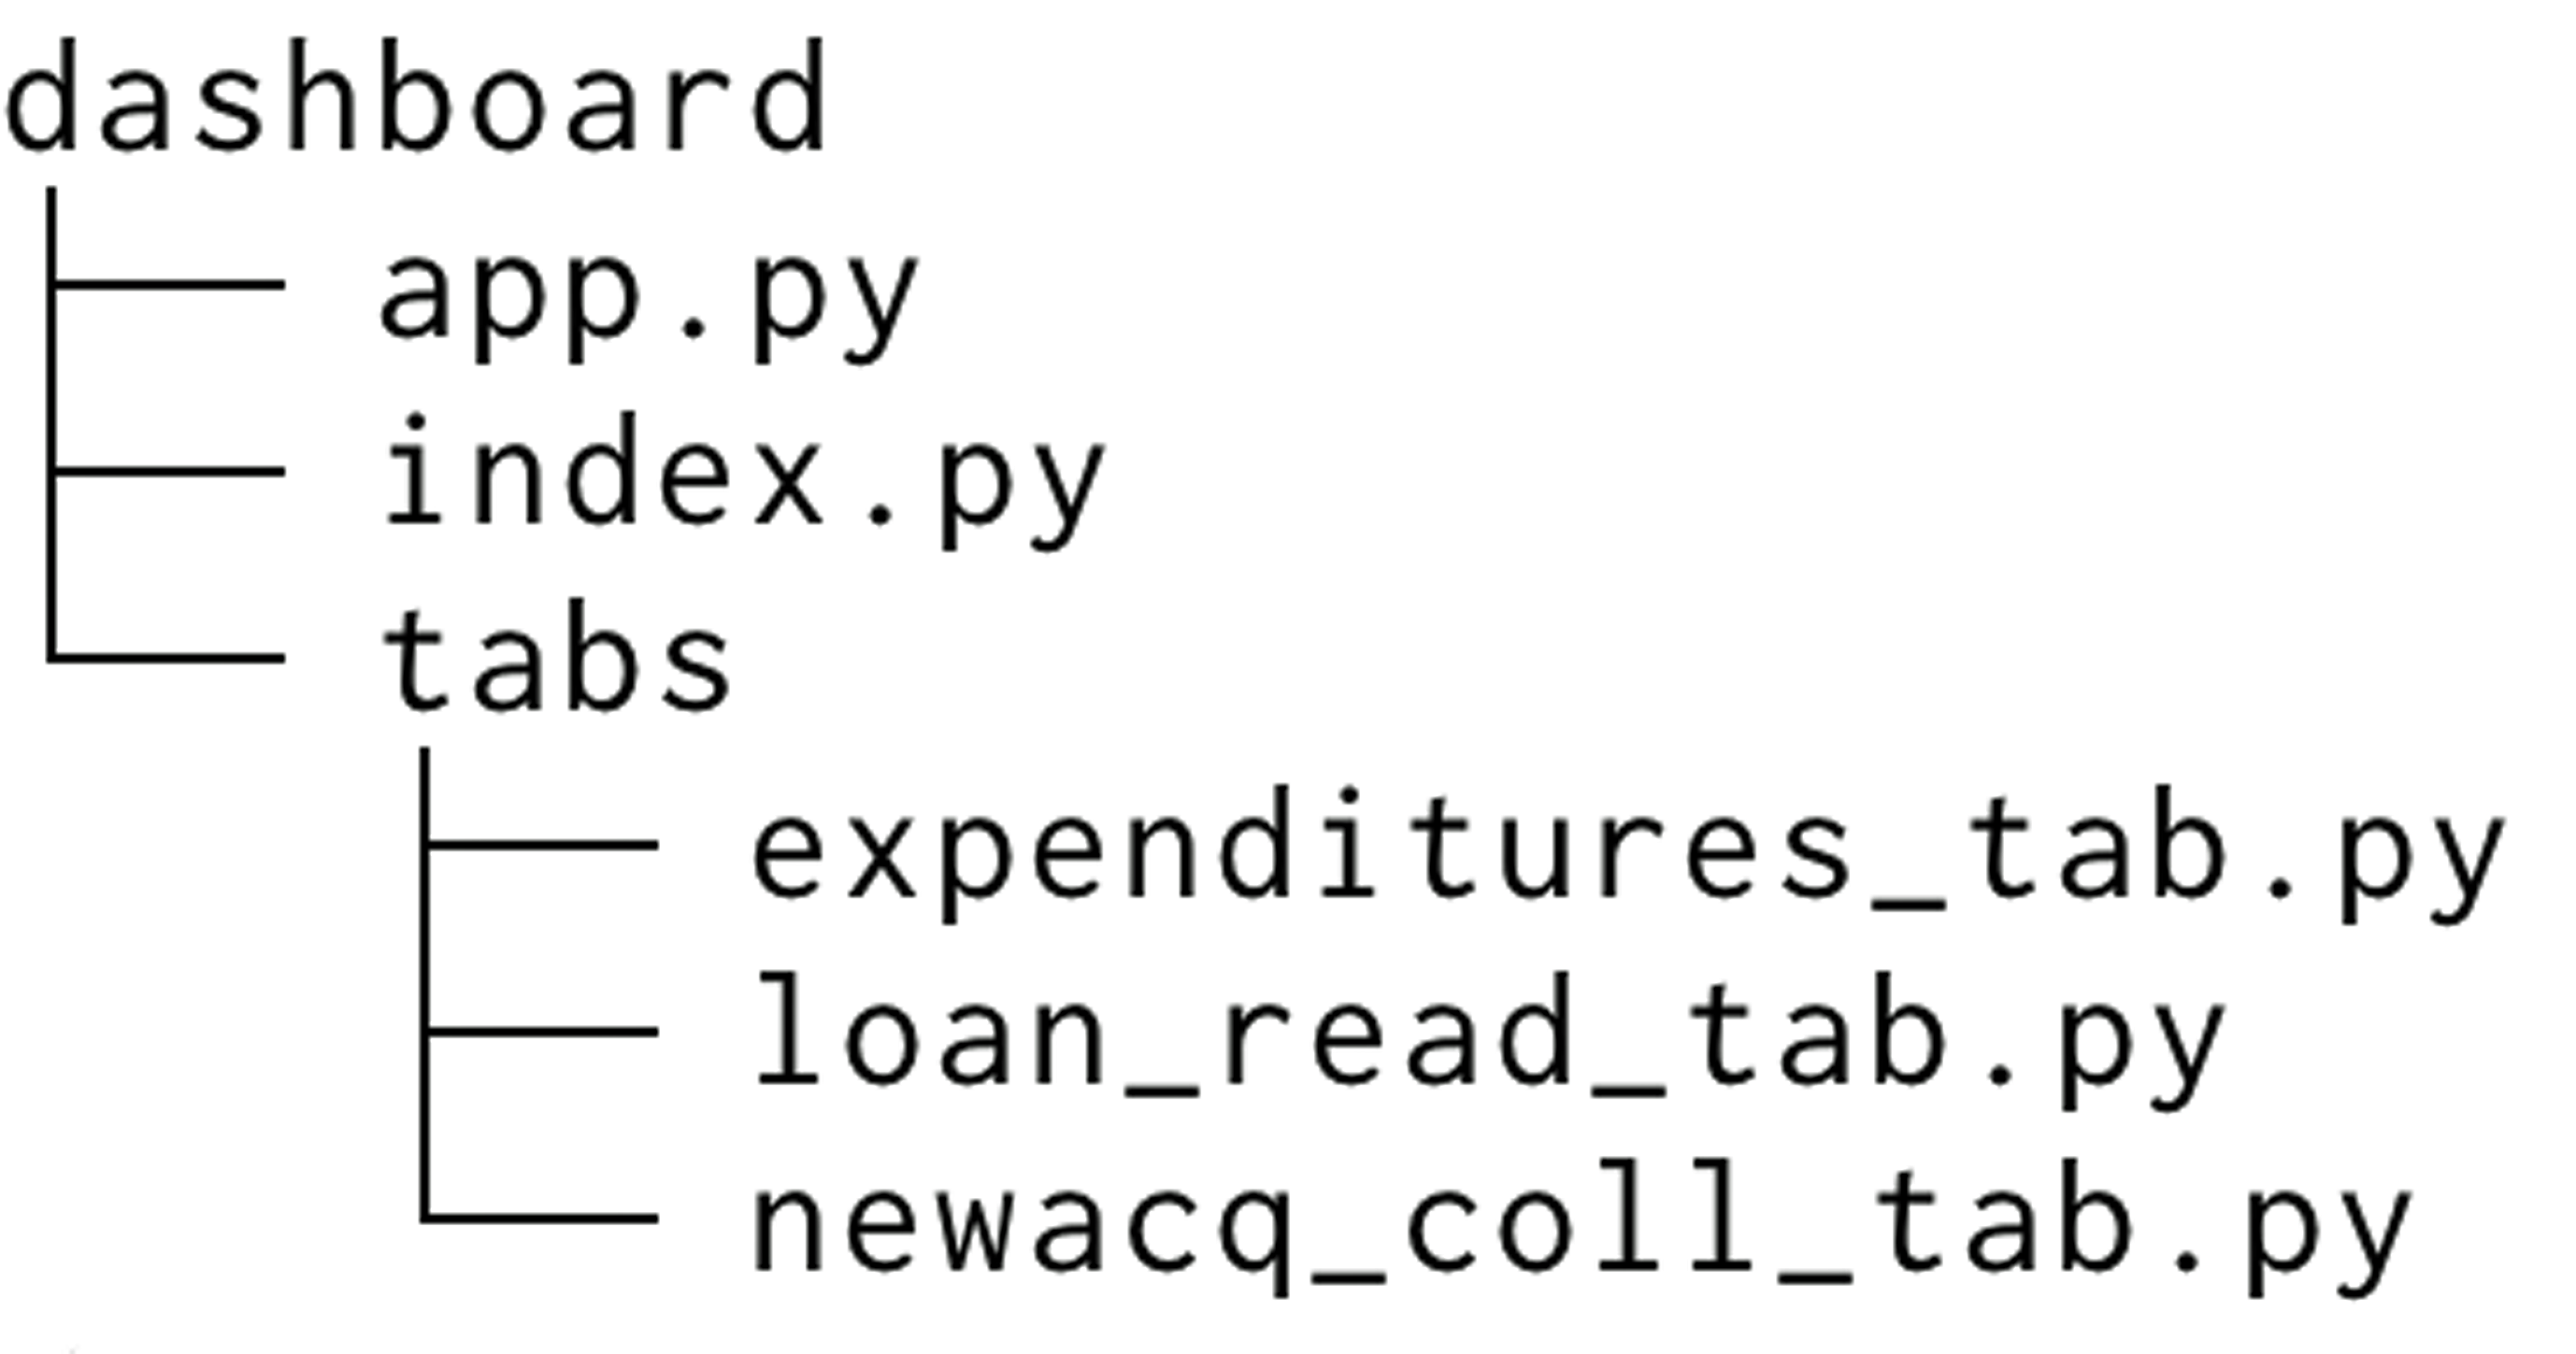
\includegraphics[width=6cm, height=4.5cm]{dash_struc}
            \caption{Struktur Dashboard App}
            \label{fig:dash structure}
    \end{figure}
    
    Dies ist eine Möglichkeit, wie sie auf der Webseite von Dash für diese Multi-App-Projekte vorgeschlagen wird \cite[vgl.][]{plotly_url_2021}.
    
    Für den Inhalt jedes einzelnen Tabs gibt es eine separate Datei.
    Die einzelnen Tabs wurden inhaltlich um bibliothekarische Basisfunktionen wie Sammeln oder Benutzen gruppiert. So werden in der \texttt{expenditures\_tab.py}
    Datenvisualisierungen erstellt, die Budget- und die Umsatzdaten visualisieren, während mit Hilfe der \texttt{loan\_read\_tab.py}
    Ausleih- und Lesesaalnutzungsdaten dargestellt werden. Mit der \texttt{newacq\_coll\_tab.py} wird ermöglicht, Daten aus dem Bereich der Bestandsentwicklung und der 
    Ausleihe zu präsentieren.

    Jede einzelne Tab-Datei besteht einerseits aus mehreren Funktionen für die Erschaffung von Datenvisualisierungen der
    Ergebnisse aus Teilsystem 2.\footnote{Zur besseren Lesbarkeit heißt die Gruppe dieser Funktionen im Folgenden \texttt{fig\_()}.}
    Innerhalb dieser Funktionen werden mit den Plotly-Funktionen Plotly Graph Object Figures geschaffen. 
    Andererseits bestehen die Dateien aus mehreren verschiedenen Funktionen für die Dash-Komponenten wie zum Beispiel Dropdown-Menüs, Cards oder Diagrammen.\footnote{Ebenfalls zur besseren Lesbarkeit
    heißt die Gruppe dieser Funktionen im Folgenden \texttt{html\_()}.}
    Diese Funktionen binden die \texttt{fig\_()}-Funktionen so ein, dass die Plotly Graph Object Figures im Dashboard zur Anzeige gebracht werden können. 
    Weiterhin sind die \texttt{html\_()}-Funktionen zum Teil mit Dekorator-Callback-Funktionen verknüpft, die es ermöglichen, mit dem Dashboard zu interagieren. 
    Ferner enthalten die Dateien jeweils eine Layoutfunktion, die das gesamte Layout des Tabs bündelt.

    Neben den Funktionen für die Dash-Komponenten und der Datenvisualisierungen, werden in den tab-Dateien noch die benötigten Objekte aus dem Modul \texttt{data\_prep} 
    instantiiert und die Methoden der Kindklassen aus diesem Modul auf diesen angewendet. In der Regel geschieht dies am Anfang 
    jeder Tab-Datei nach den Import-Anweisungen für die einzelnen Module außerhalb der Funktionen. Für die Callback-Funktionalität werden aber die Objekte und die Methoden des Moduls \texttt{data\_prep} innerhalb einiger \texttt{html\_()} aufgerufen.
    Auf den Aufbau und die Funktionsweise der Funktionen in den Tab-Dateien wird im Folgenden näher eingegangen.\footnote{Auf die Erzeugung von anderen Dash-Elementen wie Cards wird dabei aufgrund der Übersichtlichkeit der Darstellung nicht Bezug genommen. Diesem liegt ein ähnlicher Prozess
    zu Grunde. Es werden aus den berechneten Ergebnissen der Objekte direkt Dash-Komponenten mit Hilfe der \texttt{dash\_bootstrap\_components} erstellt.}
    
    Die Objekte werden zunächst in Plotly Graph Objects umgewandelt. Diese wiederum werden in Dash-Objekte transformiert und diese werden 
    letztlich in einem Tab-Layout zusammengefasst.
    \autoref{fig:process tab} zeigt schematisch die Ablauflogik in den Tab-Dateien ohne die callback-Funktionen anhand der 
    \texttt{fig\_total\_expnd()}-Funktion aus der \texttt{expenditures\_tab.py}.
    
    
    \begin{figure}[H]
        \centering
            \includegraphics[width=12cm, height=16 cm]{ablauf_tab_ps}
            %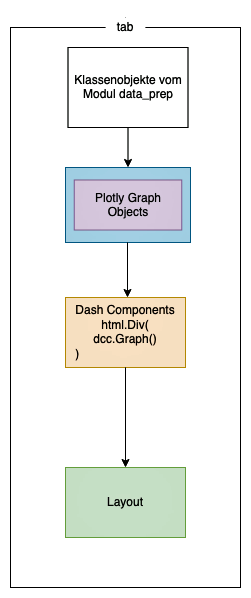
\includegraphics[width=6cm, height=8cm]{ablauf_dash_ohne_cb}
            \caption{Ablauf Tab}
            \label{fig:process tab}
    \end{figure}

    % Die grundsätzliche Logik der Funktionsaufrufe sieht in den Tab-Dateien ohne die Callback-Funktionen wie folgt aus:
    (1) Zunächst wird ein Objekt der Kindklasse \texttt{Expenditures()} aus dem \texttt{data\_prep}-Modul erzeugt 
    und auf ihn die Methode \texttt{total\_expnd\_net\_years()} ausgeführt und der Rückgabewert der Methode, der ein Dataframe entspricht, einer
    Variable zugewiesen.


    % \begin{figure}[H]
    %     \centering
    %         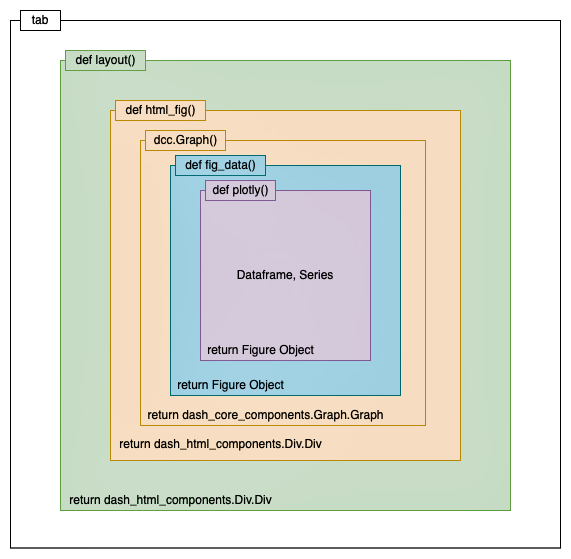
\includegraphics[width=10cm, height=8cm]{funktions_aufrufe_tab}
    %         \caption{Funktionsaufrufe Tab}
    %         \label{fig:function call tab}
    % \end{figure}

    (2) In der \texttt{fig\_}-Funktion, die das Plotly Graph Object Figure erzeugt, wird das durch die \texttt{total\_expnd\_net\_years()} erzeugte Dataframe
    als Parameter entgegengenommen. Zusätzlich müssen noch weitere Parameter übergeben werden, die für die jeweiligen Diagrammtypen wichtig sind.
    Andere Parameter, die das Layout festlegen, sind dagegen optional \cite[vgl.][]{plotly_plotlygraph_objectsbar_2021}.
    
    Im oben angegebenen Beispiel wird in der Funktion \texttt{fig\_total\_expnd()} aus \texttt{expenditures\_tab.py} ein horizontal gekipptes Figure-Objekt
    mit dem pandas Dataframe \texttt{df\_total\_expnd} durch den Aufruf der Plotly-Funktion \texttt{bar()} erstellt. 
    Es werden zusätzlich in dem Funktionsaufruf die x-Achse und y-Achse mit den Werten der Spalten \enquote{Umsatz (EUR)} und \enquote{Datum} festgelegt. 

    \begin{lstlisting}[language=Python, caption=Funktion fig\_total\_expnd() Auszug 1]
    def fig_total_expnd():
        ...
        fig = px.bar(df_total_expnd,
            x='Umsatz (EUR)',
            y='Datum',
            orientation='h',
            ...
        )
        ...
    \end{lstlisting}
    
    Weitere Funktionen von Plotly Express bearbeiten die Plotly Graph Object Figures in den \texttt{fig\_()}-Funktionen. 
    So kann durch die \texttt{update\_layout}-Funktion unter anderem der Achsentitel, die Höhe und die Breite der Datenvisualisierung 
    festgelegt werden. Als Rückgabewert der Funktionen \texttt{fig\_()} werden die Plotly Graph Object Figures zurückgegeben.

    \begin{lstlisting}[language=Python, caption=fig\_total\_expnd() Auszug 2]  
    def fig_total_expnd():
        ...
        fig.update_layout(title_x=0.5,
            xaxis_title='Umsatz (EUR)',
            yaxis_title='Jahr',
            height=500)
        fig.update_xaxes(nticks=20)         
        return fig
    \end{lstlisting}

    In dem Beispiel werden die Titel der x- und y-Achse sowie die
    Größe des Diagramm-Objektes festgelegt. Schließlich wird noch die x-Achse mit der Funktion \texttt{update\_xaxes()} skaliert.
    
    (3) Die \texttt{fig\_()}-Funktionen werden durch die Graph-Komponente der \texttt{dash\_core\_components} (dcc.Graph) innerhalb der 
    \texttt{html\_()}-Funktionen aufgerufen. Diese Komponente ist für die Umsetzung der interaktiven Datenvisualisierungen 
    zuständig. Ebenfalls kann von der Graph-Komponente eine \texttt{id} als Parameter entgegengenommen werden. 
    Diese ist unter anderem wichtig für die eindeutige Adressierung durch die Callback-Funktionen.
    Zudem werden in den \texttt{html\_()}-Funktionen durch die \texttt{dash\_html\_components} die Eigenschaften und 
    das Aussehen der Div-Objekte definiert. 
    Dabei werden die Properties unter anderem in der externen css-Datei \texttt{layout.css} definiert, die in dem Verzeichnis \texttt{assets} 
    des Dashboard-Verzeichnisses liegt.

    \begin{lstlisting}[language=Python, caption={html\_fig\_total\_expnd()}] 
        def html_fig_total_expnd():
        ...
        return html.Div(
            [
                html.Div(
                    [
                        dcc.Graph(
                            id='gesamtumsatz',
                            figure=fig_total_expnd()
                        ),
                    ], className="six columns chart_div", style={'margin-top': '20px', 'margin-left': '10px'}
                ),
            ]
        )
        \end{lstlisting}
    
    (4) Die \texttt{html\_()}-Funktionen werden schließlich in einer Layoutfunktion eingebunden, die alle \texttt{html\_()}-Funktionen
    für das Gesamtlayout des Tab bündelt. Als Rückgabewert returniert sie ebenso wie die \texttt{html\_()}-Funktionen ein Div-Objekt der \texttt{dash\_html\_components}.\\



    Die Callback-Funktionen wurden für zwei Dropdown-Menüs in zwei Tab-Dateien implementiert.
    Die Werte der Dropdown-Menüs werden aus den uniquen Werten einer Dataframespalte erstellt.
    Der Callback ist als Dekorator für jeweils eine Funktion implementiert. 
    In der Implementierung wird ein Callback ausgelöst, wenn ein Wert über das Dropdown-Menü ausgewählt wird.
    Im Programmcode wird das für ein Diagramm der Lesesaalnutzung in der \texttt{loan\_read\_tab.py} folgendermaßen umgesetzt.

    \begin{lstlisting}[language=Python, caption={html\_fig\_total\_expnd()}]        
    
    @app.callback(
    Output(component_id='use_by_month', component_property='figure'),
    [Input(component_id='my-id2', component_property='value')])
    def update_output_div(input_value):
    ...
    return fig_use_by_month(input_value)
    \end{lstlisting}

    % Die Funktionsweise der Callback-Funktionen zeigt die \autoref{fig:process tab_dash_cb}.

    % \begin{figure}[H]
    %     \centering
    %         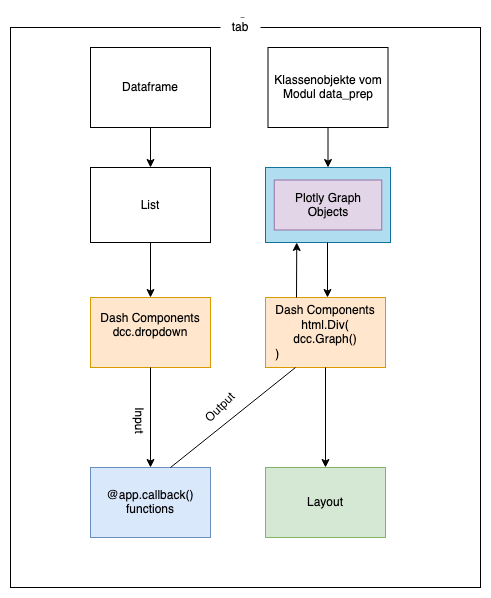
\includegraphics[width=8cm, height=10cm]{ablauf_dash_mit_cb}
    %         \caption{Ablauf Tab mit Callback}
    %         \label{fig:process tab_dash_cb}
    % \end{figure}
 
    Der Callback übergibt den Wert (input\_value) des Dropdown-Menüs an die Funktion \texttt{update\_output\_div()}. 
    Die Funktion gibt das Ergebnis einer \texttt{fig\_()}-Funktion mit diesem Wert als Argument zurück.\footnote{Diese Funktionen übergeben den Methoden der Kindklassen aus dem Modul \texttt{data\_prep} das Argument. 
    Diese erzeugen einen Dataframe basierend auf den übergebenden Argument und geben mit Hilfe der Plotly-Funktionen ein Plotly Graph Object Figure der gefilterten Daten zurück.}
    Der Callback \texttt{@app.callback} übergibt das zurückgegebene Ergebnis an die im Output angegebene Komponente.
    
    Input() und Output() nehmen die id einer Komponente und die Eigenschaft einer Komponente als Argumente entgegen.
    Die Inputkomponente ist in dem Beispiel die Dropdown-Komponente, während die Outputkomponente die dcc.Graph-Komponente der
    \texttt{html\_use\_by\_month()} darstellt. Beide werden über die eindeutige \texttt{component\_id} adressiert.
    Multiple Inputs and Outputs sind ebenfalls möglich. So sind in der \texttt{expenditures\_tab.py}
    jeweils zwei Diagramme und Zahlenwerte für den Umsatz von den Werten einer Dropdown-Liste abhängig.
    % Dabei handelt es sich um Methoden, die die Daten nach einem Wert filtern und die vom Wert der Dropdown-Liste abhängig sind. Deswegen wird bei diesen
    % Plotly-Funktionen in der Tab-Datei der Wert der Dropdown-Liste als Argument mit in die Funktion gegeben.
    In der \autoref{fig:process tab_dash_cb} ist die Ablauflogik in den Tab-Dateien mit der Callback-Funktion skizziert.

    \begin{figure}[H]
        \centering
            \includegraphics[width=12cm, height=10cm]{ablauf_tab_cb_ps}
            \caption{Ablauf Tab mit Callback}
            \label{fig:process tab_dash_cb}
    \end{figure}


    Zusammengesetzt wird das Layout des Dashboards durch den Aufruf der Layout-Funktion der einzelnen Tab-Dateien in der \texttt{index.py}.
    Die \texttt{index.py} definiert zudem das Layout des gesamten Dashboards. Hier werden auch die Anzahl und die Eigenschaften der Tabs festgelegt. 
    Die Dekorator-Callback-Funktion \texttt{@app.callback()} steuert die Auswahl der Tabs und ruft die jeweiligen Tabs beziehungsweise deren 
    Layouts auf. \autoref{fig:process tab_dash_cb} zeigt die Funktionsweise einer Tab-Datei mit der \texttt{index.py}.

    \begin{figure}[H]
        \centering
            \includegraphics[width=15cm, height=10cm]{ablauf_tab_cb_ind_ps}
            \caption{Ablauf Tab mit index}
            \label{fig:process tab_dash_cb}
    \end{figure}

    Der Einstiegspunkt zur Ausführung des Dashboards ist die Datei \texttt{index.py}. Mit dieser Datei wird das Dashboard mittels \texttt{Flask-Webserver}
    gestartet. Zur Vermeidung zirkulärer Importe ist die Dash-Instanz in der separaten \texttt{app.py} definiert \cite[vgl.][]{plotly_url_2021}.


    %\textit{Standardbericht}\\

\section{Demonstration der Funktionalität}

    Im Folgenden wird die Funktionsweise des Systems dargelegt. 
    Dabei wird zunächst auf die technischen Voraussetzungen eingegangen, und dann spezifisch das Teilsystem 1 Import erläutert, und schließlich der
    praktische Import der Daten skizziert. Da das Teilsystem 2 keine Schnittstelle
    nach außen bietet, wird auf dieses nicht eingegangen. Das Teilsystem 3 ist insofern interessant, da von diesem das Dashboard
    gestartet wird. Das Dashboard ist die grafische Umsetzung des Teilsystem 2 und Teilsystem 3. Beim Dashboard wird kurz auf das Layout
    eingegangen, bevor die Funktionsweise und die Datenvisualisierungen besprochen werden.


    \subsection{Technische Voraussetzungen}
    Der Programmcode zum Projekt ist auf GitHub zu finden.\footnote{\url{https://github.com/pbretern/library-dashboard-system}} Dort gibt es weitere Informationen zur Installation.
    Das System wurde auf den Betriebssystemen macOS Big Sur, Linux in der Ubuntu-Distribution 20.10. getestet.
    Das Dashboard kann mit den aktuellen Versionen der Web-Browser Google Chrome, Firefox und Safari dargestellt werden. 
    Als Hardware-Anforderungen wird ein Intel Dual Core i5 (Haswell) mit 128 GB Festplatte und 8 GB Arbeitsspeicher angegeben. 
    Mit dem Programmcode werden keine bibliothekarischen Daten mitgeliefert.\footnote{Testdaten werden eventuell nach der Veröffentlichung des Repositoriums
    sukzessive zur Verfügung gestellt.}
    
    \subsection{Daten-Import}
    Der Import der Daten findet über Skripte statt. Diese liegen im Projektverzeichnis \texttt{src/instances}.
    Für Budget, Umsatz, Neuerwerbungen und Ausleihdaten liegen einzelne Python-Skripte bereit, die manuell über die Kommandozeile
    aufgerufen werden können. Zudem gibt es noch ein shell-Skript, das die vier Skripte zusammen auslöst. Dieses
    muss ebenfalls manuell aufgerufen werden.
    Beim Import wird eine Meldung über die Anzahl der zu importierenden Daten auf der Kommandozeile angezeigt. 
    Nach erfolgreichem Abschluss des Imports wird zudem eine einfache Erfolgsmeldung auf der Kommandozeile ausgegeben.
    %\footnote{Es gibt Warnungen, die angezeigt werden. Diese Warnmeldungen haben keinen Einfluss auf den Import. Im Bearbeitungszeitraum der Arbeit konnte diesen Warnmeldungen leider nicht nachgegangen werden.}

    Die Pfade zu den lokalen Verzeichnissen für Import und Speicherung der Daten sind als Konstanten zentral in der \texttt{configuration.py}
    im Projektverzeichnis hinterlegt. Dort sind auch noch andere Pfadkonstanten definiert, die auf Dateien für die Datenanreicherung verweisen, welche das Teilsystem 1
    und das Teilsystem 2 unterstützen. Wichtig ist, dass die zu importierenden Daten über Dateinamen einer gewissen Semantik und 
    über ein gewisses Format verfügen müssen, sonst werden sie nicht importiert (Siehe auch \autoref{chap:five_one_three} Teilsystem 1).

    \subsection{Dashboard}
    Gestartet wird die Dashboard-Applikation auf der Kommandozeile, indem \texttt{index.py} im Projektverzeichnis \texttt{dashboard}
    aufgerufen wird. Diese startet den Flask-Webserver mit der Dashboard-App. Der Webserver ist in der \texttt{index.py} so eingestellt, 
    dass er alle Netzwerkschnittstellen abhört.


    \begin{figure}[H]
        \centering
            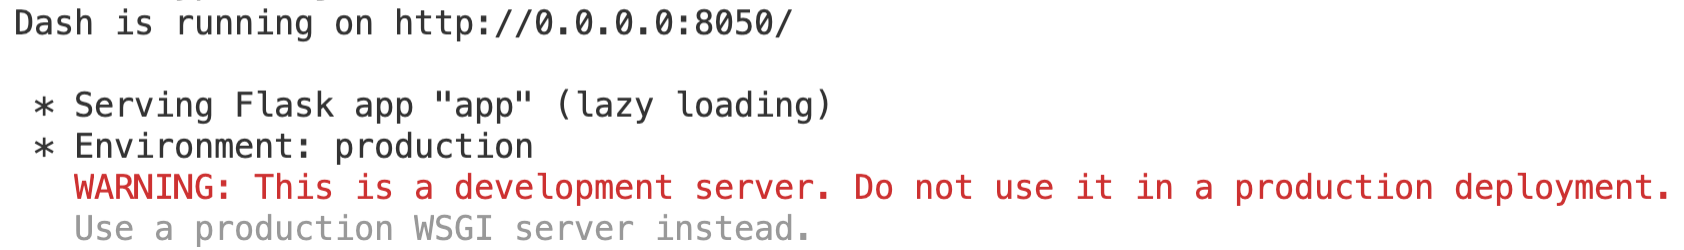
\includegraphics[width=12cm, height=2cm]{flask_webserver}
            \caption{Start Flask Webserver}
            \label{fig:flask}
    \end{figure}

    % Wie im \autoref{chap:five_one_three} Teilsystem 3 beschrieben besteht das Dashboard aus drei Tabs.
    % Die Navigation zu den drei Tabs ist im oberen Bereich des Dashboards nebeneinander angeordnet. 
    
    % \begin{figure}[H]
    %     \centering
    %         
\includegraphics[width=14cm, height=2cm]{tabs}
    %         \caption{Tabs-Navigation}
    %         \label{fig:flask}
    % \end{figure}
    Das Dashboard kann mit der angegebenen Adresse vom Web-Browser geöffnet werden.
    \autoref{fig:Struktur Layout} zeigt schematisch die Layout-Struktur des Dashboards. 


    \begin{figure}[H]
        \centering
            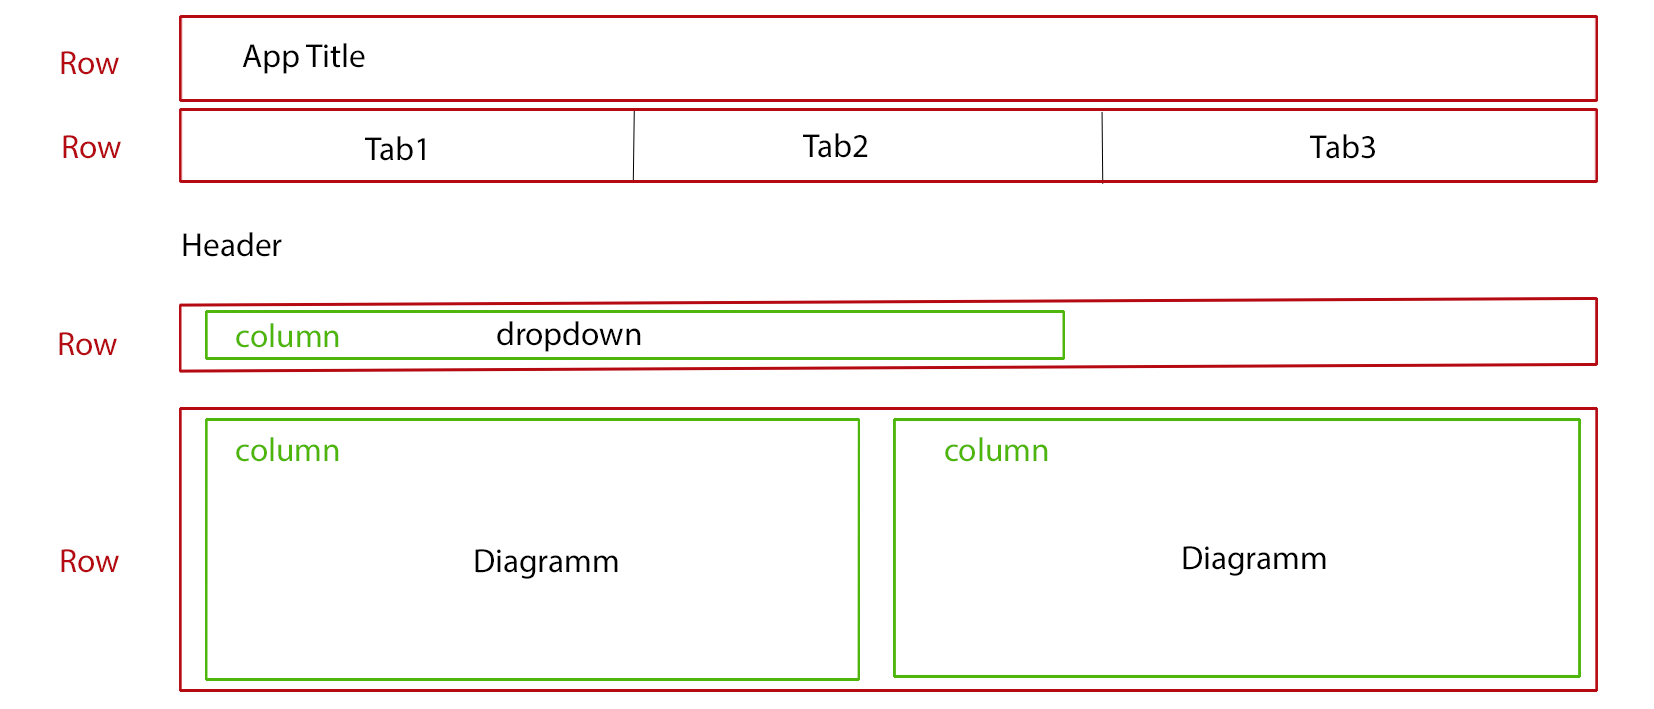
\includegraphics[width=14cm, height=6cm]{layout_abstr}
            \caption{Struktur Layout}
            \label{fig:Struktur Layout}
    \end{figure}


    Die Layout-Struktur besteht aus Divs, Rows, Header und Columns, den Steuerelementen wie Dropdown-Menüs sowie den Darstellungselementen wie Diagrammen, Tabellen
    oder Cards. Die einzelnen Rows werden durch Div-Container bemantelt. Diese sind auf dem html-Body angesiedelt.
    Während die ersten beiden Rows zentral in der \texttt{index.py} festgelegt werden, werden die anderen Rows in den einzelnen Tab-Dateien definiert. 
    Diese Rows beherbergen bis zu drei Columns-Elemente, in denen die Steuer- und Datenvisualisierungselemente enthalten sind.
    Die Columns-Elemente sind in Abhängigkeit der darzustellenden Daten unterschiedlich groß. 
    Die Größe wird festgelegt in den einzelnen \texttt{fig\_()}-Funktionen des Teilsystems 3.
    Die Header gelten als inhaltlicher Trenner zwischen den einzelnen Datenvisualisierungen und dienen der schnelleren Orientierung. 
    Die Header sind zudem mit der jeweils nachfolgenden Row verknüpft. Das Dashboard besteht aus drei Tabs: \textit{Umsatz und Budget}, 
    \textit{Lesesaal und Ausleihe}, \textit{Neuerwerbungen und Bestand}. Der Wechsel zwischen den Tabs geschieht durch das einmalige
    Klicken mit der Maus auf dem Tab-Titel. Nachdem die Adresse im Browser geöffnet wurde, wird der Tab \textit{Umsatz und Budget} aufgerufen. Dieser ist
    als default-value im Dashboard-Layout der \texttt{index.py} eingestellt. Im Folgenden werden die Tabs per screenshot abgebildet sowie 
    die in ihnen enthaltenen Informationen tabellarisch dargestellt. Die tabellarische Darstellung richtet sich dabei an den Rows der Layout-Struktur aus. 

    %\clearpage
    \noindent
    \textit{Tab1 - Umsatz und Budget}
    %Den Tab \textit{Umsatz und Budget} zeigt \autoref{fig:tab1}
    \footnote{Für die Darstellung der Umsatz- und
    Budgetdaten werden sowohl die Kostenstellen als auch die Lieferanten maskiert dargestellt. Es wurde außerdem mit Testdaten
    gearbeitet, die bis März 2021 gehen.}

    \KOMAoptions{paper=A3,paper=portrait}
    \recalctypearea
    
    \textit{Tab1 - Umsatz und Budget}
    \footnote{Für die Darstellung der Umsatz- und
    Budgetdaten werden sowohl die Kostenstellen als auch die Lieferanten maskiert dargestellt. Es wurde außerdem mit Testdaten
    gearbeitet, die bis März 2021 gehen.}
    %\begin{sidewaysfigure}
    \begin{figure}[H]
        \centering
            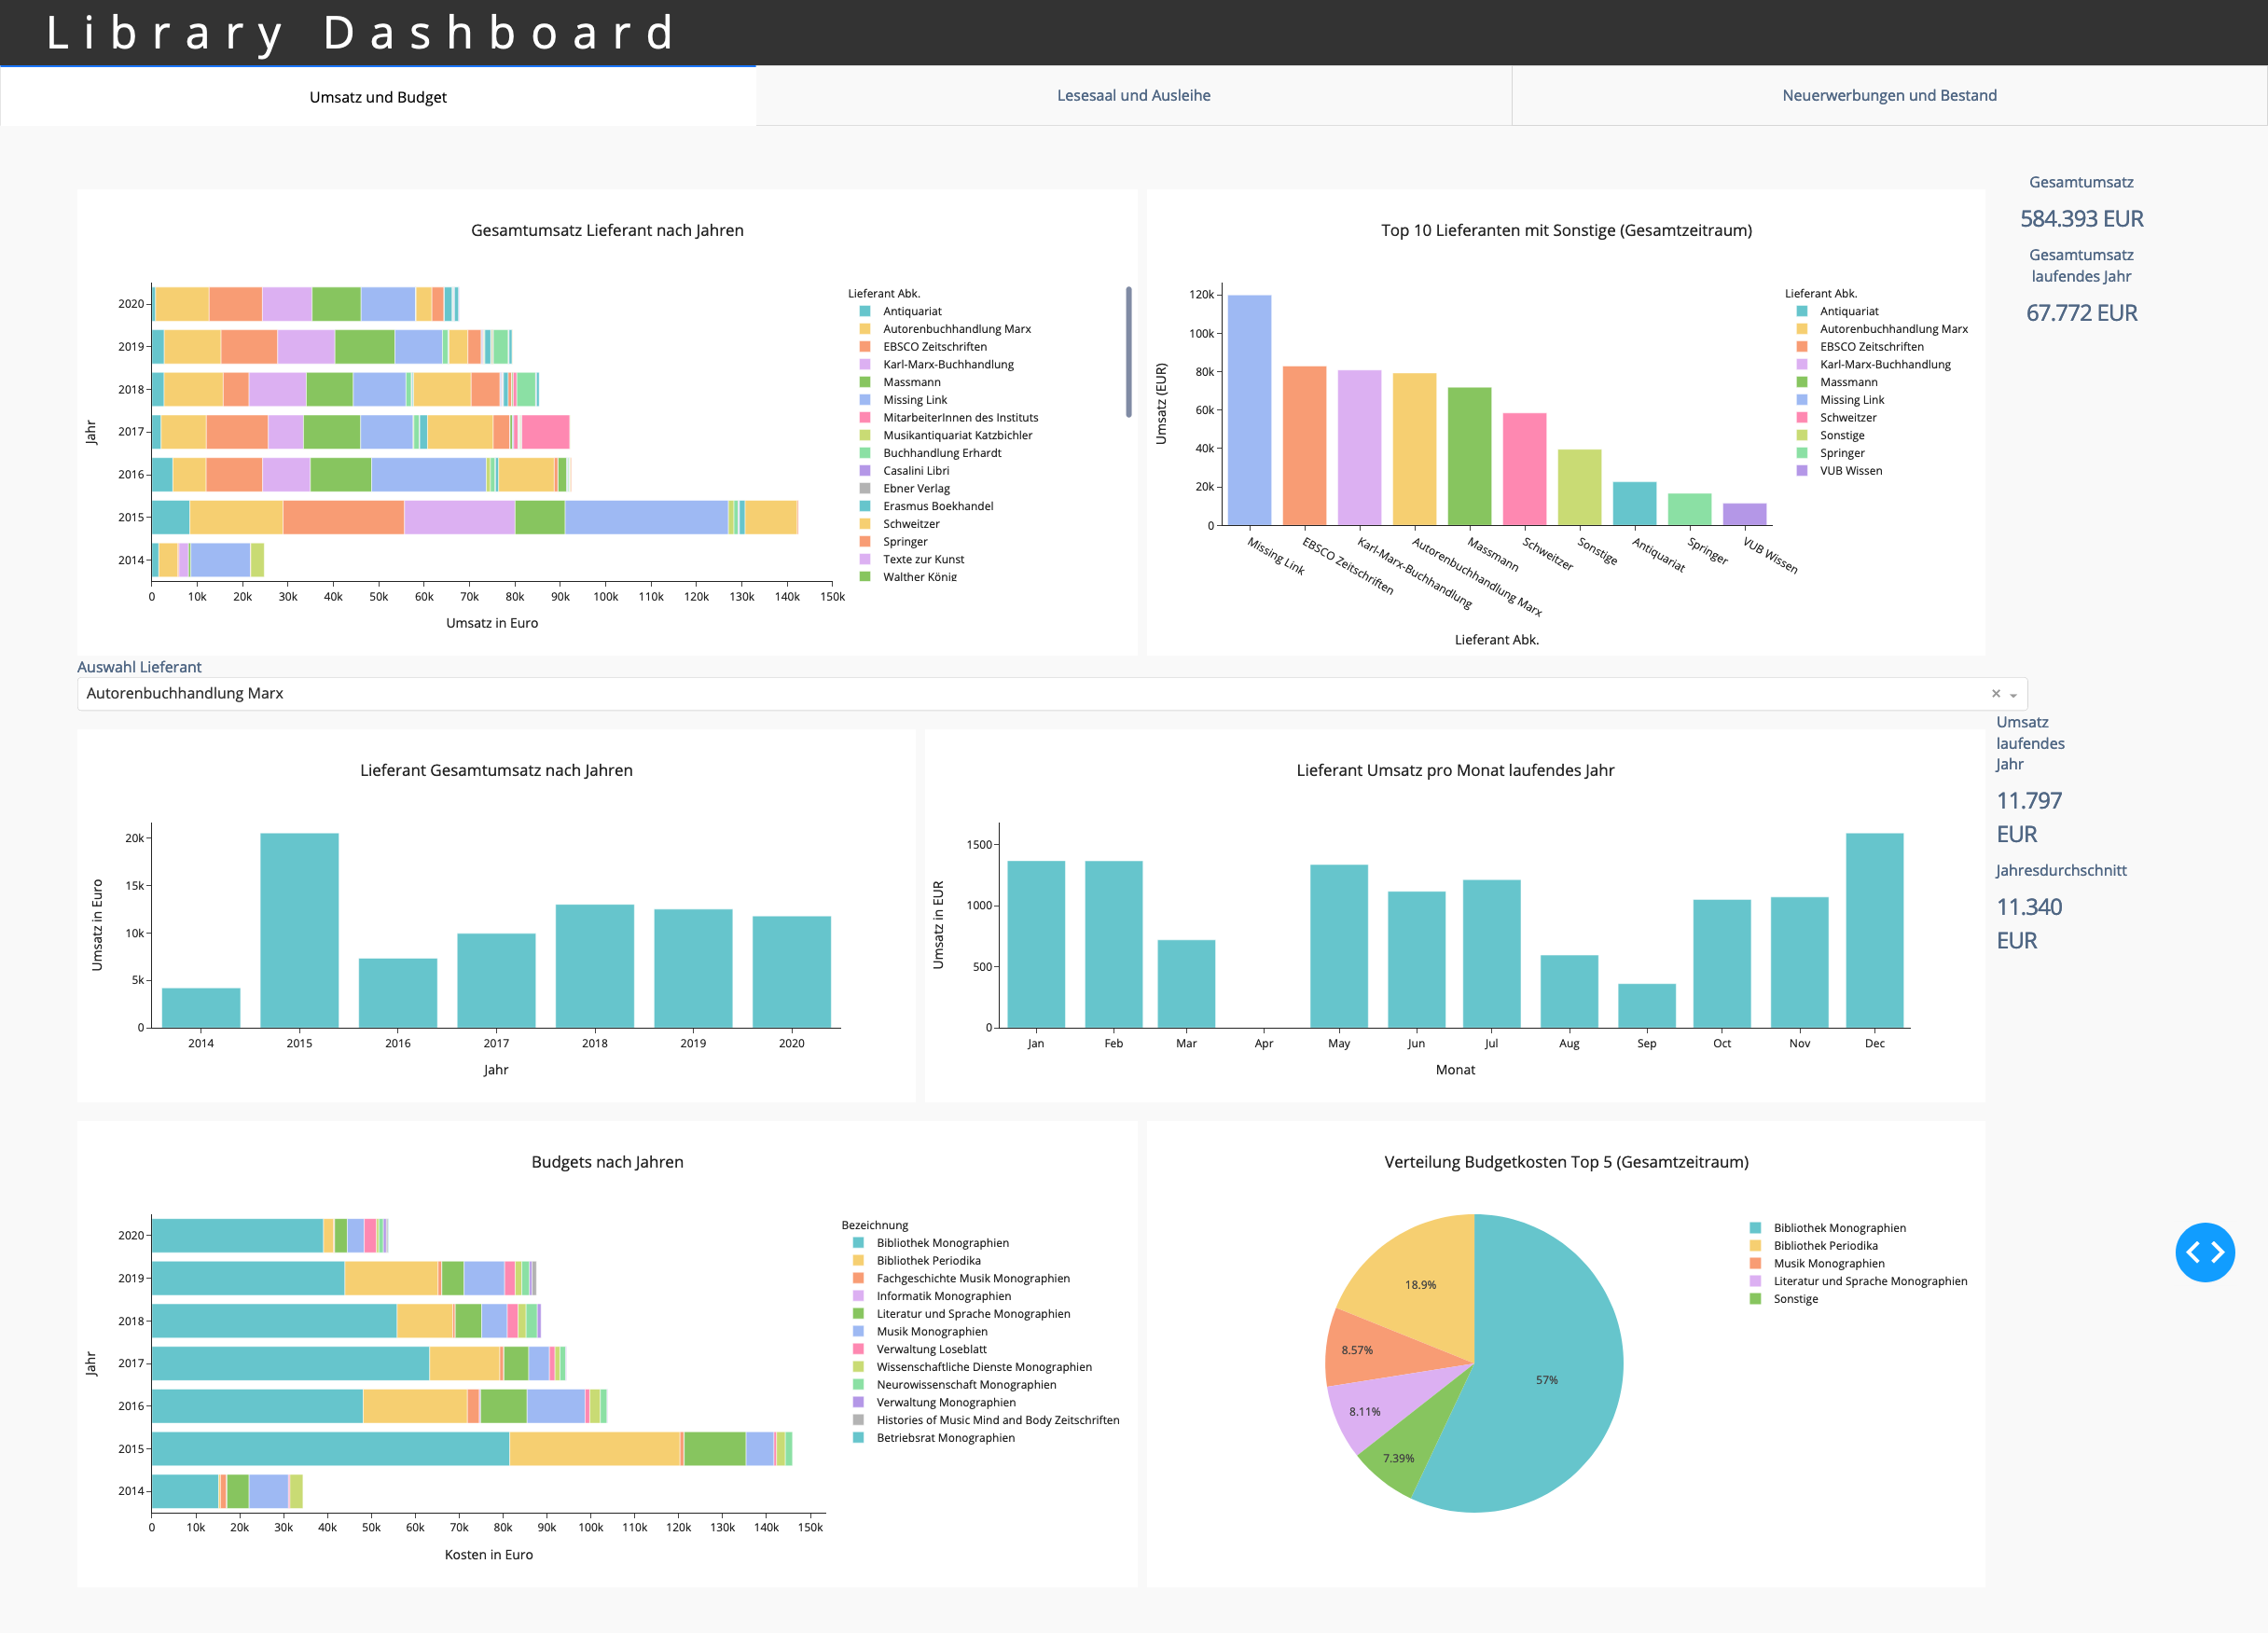
\includegraphics[width=22cm, height=26 cm]{tab1}
            \caption{Tab1}
            \label{fig:tab1}
    \end{figure}
    %\end{sidewaysfigure}

    % Genug A3 fürs erste. Jetzt ein Seitenumbruch und dann wieder A4-Format:
    \clearpage
    \KOMAoptions{paper=A4,paper=portrait}
    \recalctypearea  
    %Folgende Diagramme und Steuerelemente werden im Tab \textit{Umsatz und Budget}.
    \begingroup
    \setlength{\tabcolsep}{12pt} % Default value: 6pt
    \renewcommand{\arraystretch}{1.5}
    \begin{table}[h]
        \LARGE
        \centering
        \begin{adjustbox}{max width=\textwidth}
        \begin{tabular}{p{0.1\textwidth}p{0.5\textwidth}p{0.4\textwidth}p{0.25\textwidth}p{0.4\textwidth}p{0.5\textwidth}}
           \toprule
           Row        &Titel der Darstellungen&Beschreibung &Datenset &Darstellung &Interaktivität auf dem Dashboard\\
           \midrule
            1           &Gesamtumsatz Lieferanten nach Jahren &Die Einzelwerte der Lieferanten pro Jahr werden dargestellt.   &Umsatzdaten    &gestapeltes Balkendiagramm (horizontal)    &Plotly-Interaktivität (Aus- und Einblenden von Balken, Hover-Informationen)\\
                        &Top 10 Lieferanten mit Sonstige &Die 9 Lieferanten, bei denen der Umsatz am stärksten ist, werden dargestellt. Die restlichen werden in Sonstiges gruppiert.   &Umsatzdaten    &Balkendiagramm    &Plotly-Interaktivität (Aus- und Einblenden von Balken, Hover-Informationen)\\
                        &Gesamtumsatz&-&Umsatzdaten    &numerischer Wert   &-\\
                        &Gesamtumsatz laufendes Jahr&-&Umsatzdaten    &numerischer Wert   &-\\
            
                        \midrule
            2           &Auswahl  Lieferant &Dropdown-Menü mit eindeutigen Werten der Dataframe-Spalte \enquote{Lieferanten Abk.}&Umsatzdaten&Dropdown-Menü &Auswahl von Werten aus einer Liste. Dadurch werden vier Darstellungen im Tab beeinflusst.\\
            \midrule
            3           &Gesamtumsatz Lieferant nach Jahren&Der Gesamtumsatz eines Lieferanten nach Jahren wird dargestellt.   &Umsatzdaten    &Balkendiagramm    &Auswahl des Lieferanten über das Dropdown-Menü\\
                        &Lieferant Umsatz pro Monat laufendes Jahr&Der Gesamtumsatz eines Lieferanten nach Monaten für das laufende Jahr wird dargestellt.   &Umsatzdaten    &Balkendiagramm    &Auswahl des Lieferanten über das Dropdown-Menü.\\
                        &Umsatz laufendes Jahr (für einen Lieferanten)&- &Umsatzdaten    &numerischer Wert    &Wert verändert sich durch Auswahl des Lieferanten über das Dropdown-Menü.\\
                        &Jahresdurchschnitt (Lieferant)&- &Umsatzdaten    &numerischer Wert    &Wert verändert sich durch Auswahl des Lieferanten über das Dropdown-Menü\\
            \midrule
            4           &Gesamtbudget Kostenstellen nach Jahren&Die Einzelwerte der Kostenstellen pro Jahr werden dargestellt.&Budgetdaten    &gestapeltes Balkendiagramm (horizontal)    &Plotly-Interaktivität (Aus- und Einblenden von Balken, Hover-Informationen)\\
                        &Top 5 Kostenstellen mit Sonstige&Die 4 Kostenstellen, bei den die Budgetkosten am größten sind, werden dargestellt. Die restlichen werden in der Sonstiges gruppiert. &Budgetdaten    &Kreisdiagramm    &Plotly-Interaktivität (Aus- und Einblenden von Anteilen, Hover-Informationen)\\

        \bottomrule
        \end{tabular}
        \end{adjustbox}
        \caption
        \end{table}
    \endgroup
    


\clearpage
\KOMAoptions{paper=A3,paper=portrait}
\recalctypearea
\textit{Tab2 - Lesesaal und Ausleihe}
%Den Tab \textit{Lesesaal und Ausleihe} zeigt \autoref{fig:tab2}.
    \begin{figure}[H]
        \centering
            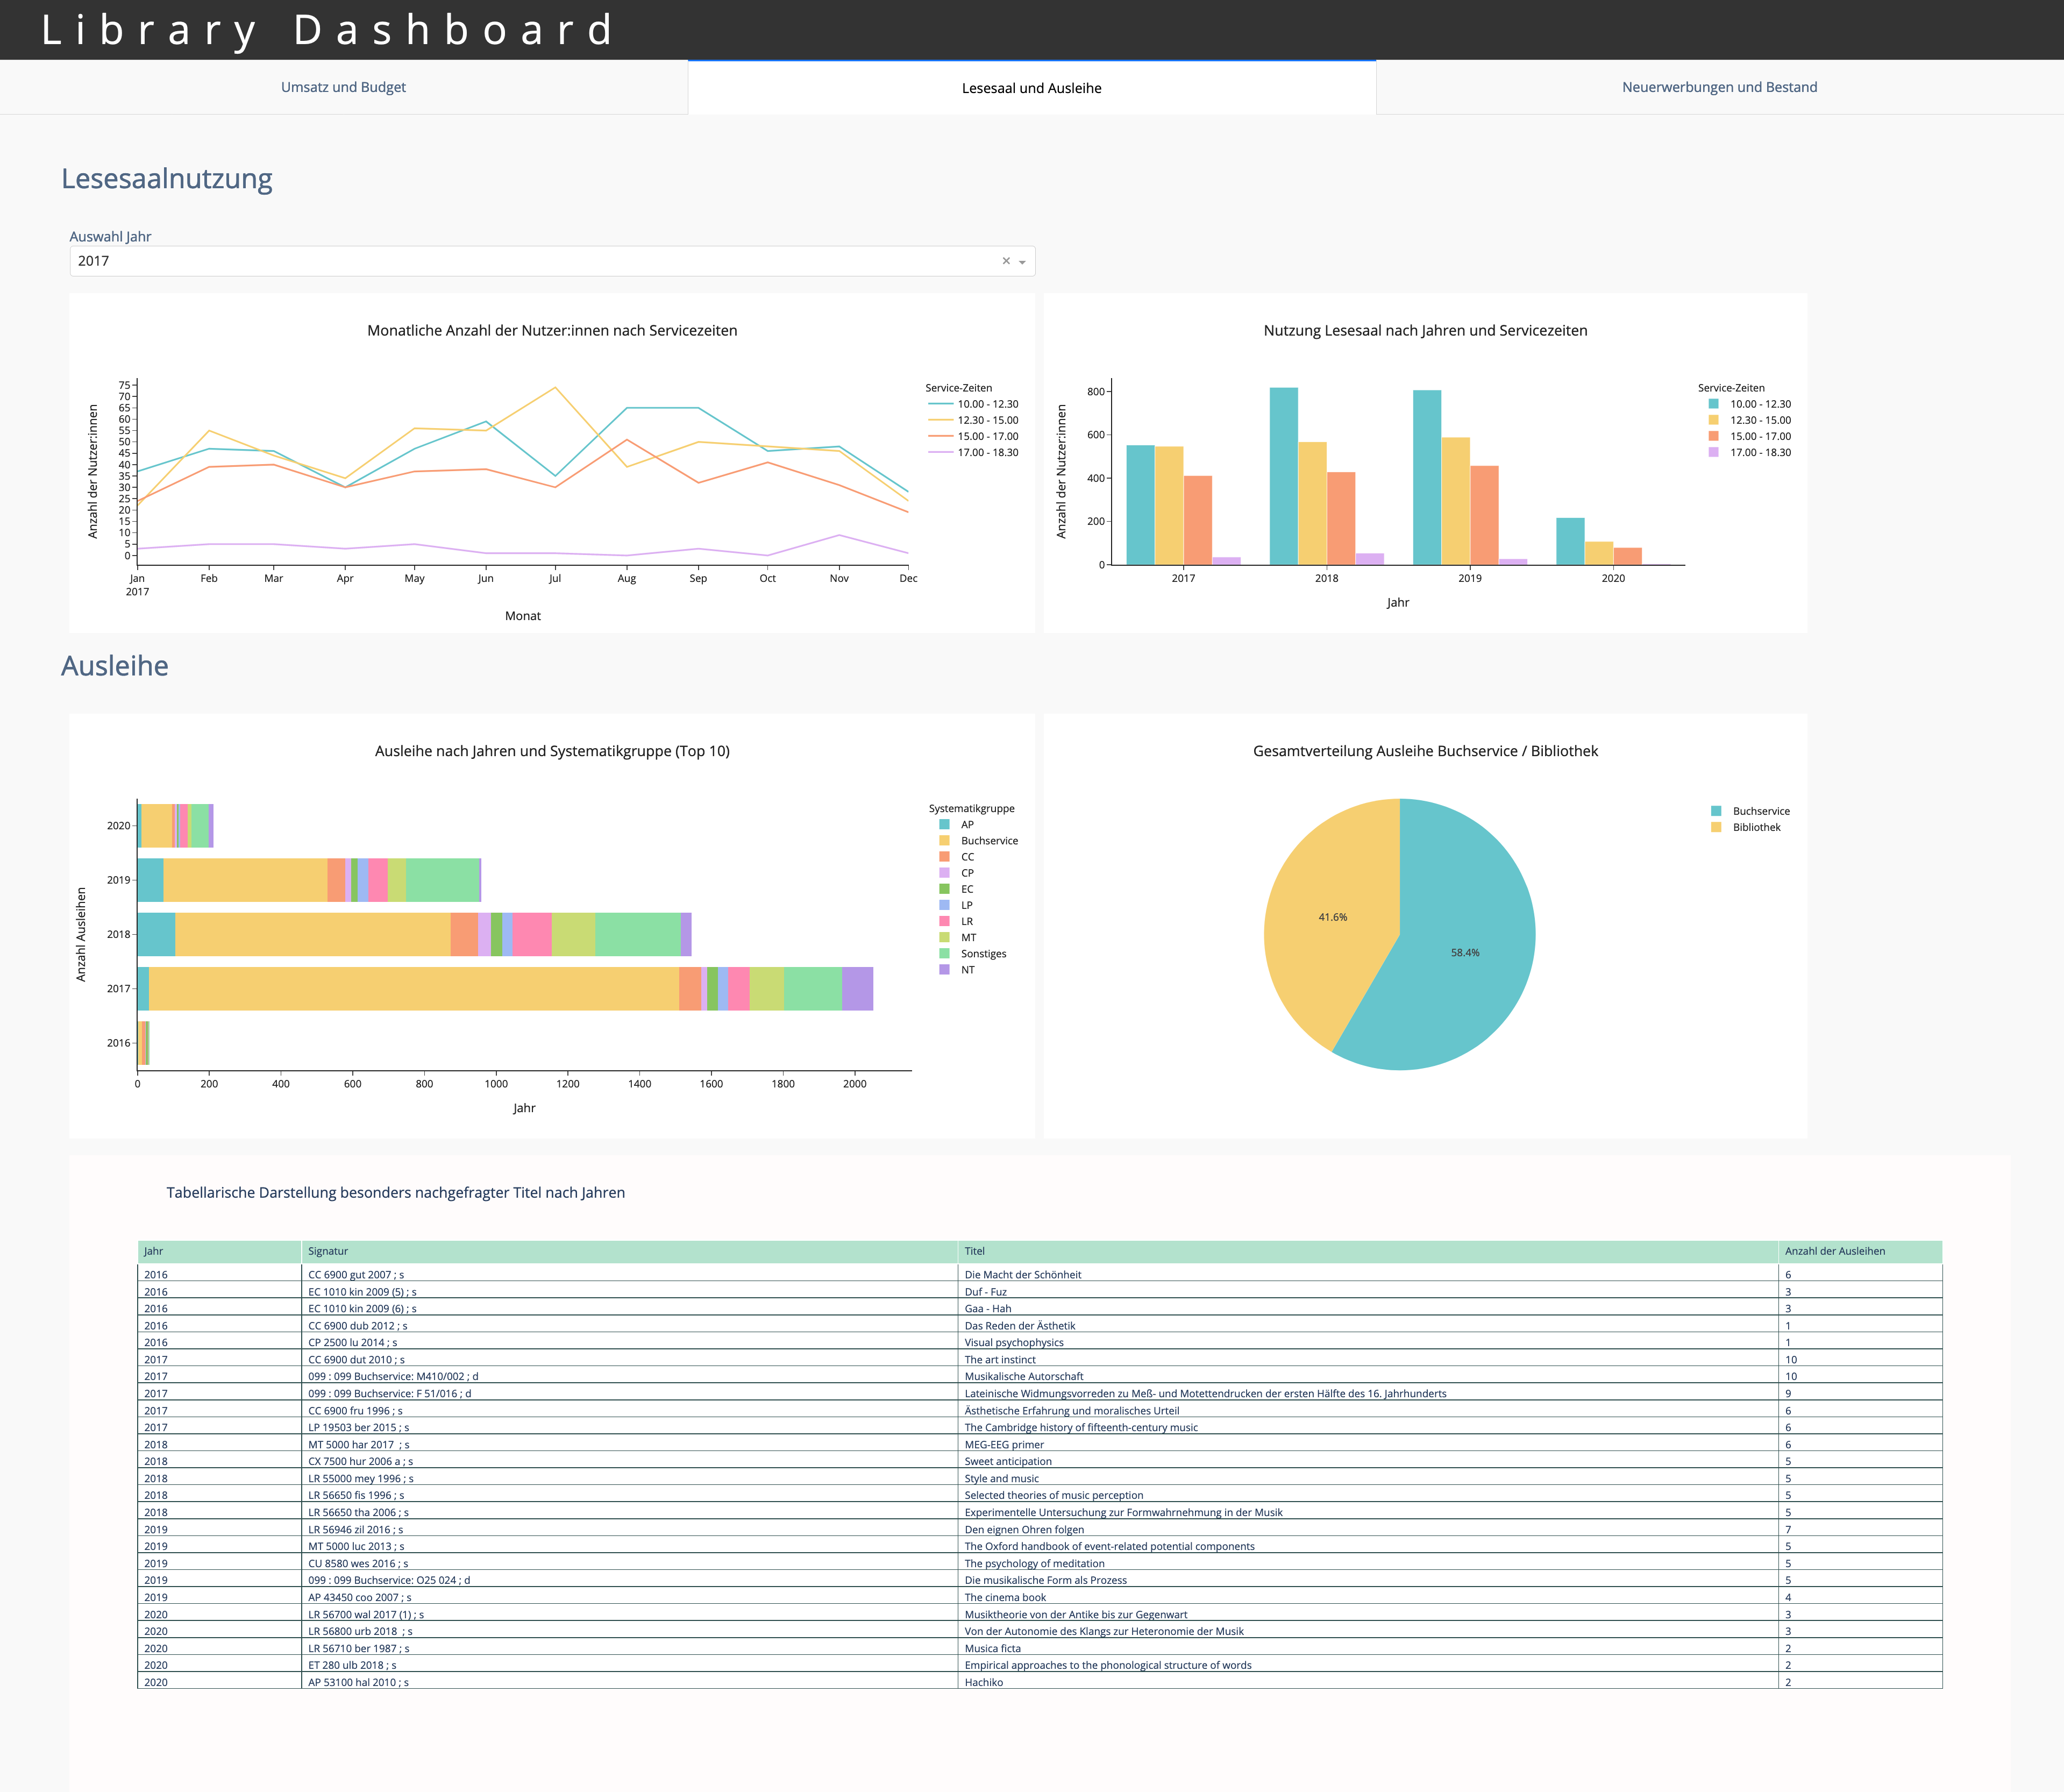
\includegraphics[width=22cm, height=26cm]{tab2}
            \caption{Tab2}
            \label{fig:tab2}
    \end{figure}

\clearpage
\KOMAoptions{paper=A4,paper=portrait}
\recalctypearea  

%\clearpage
%Folgende Diagramme, Tabellen und Steuerelemente werden im Tab \textit{Lesesaal und Ausleihe} dargestellt.
    \begingroup
    \setlength{\tabcolsep}{12pt} % Default value: 6pt
    \renewcommand{\arraystretch}{1.5} 
    \begin{table}[h]
        \LARGE
        \centering
        \begin{adjustbox}{max width=\textwidth}
        \begin{tabular}{p{0.1\textwidth}p{0.5\textwidth}p{0.4\textwidth}p{0.3\textwidth}p{0.4\textwidth}p{0.4\textwidth}}
           \toprule
           Row        &Titel der Darstellungen&Beschreibung &Datenset &Darstellung &Interaktivität auf dem Dashboard\\
           \midrule
            1           &Auswahl  Jahr &Dropdown-Menü mit eindeutigen Werten der Dataframe-Spalte \enquote{Jahr}.&Ausleihdaten&Dropdown-Menü &Auswahl von Werten aus einer Liste. Dadurch wird eine Darstellung beeinflusst.\\
           \midrule
            2           &Monatliche Anzahl der Nutzer:innen nach Service-Zeiten&Es wird der monatliche Verlauf pro Jahr nach den vier Service-Zeiten dargestellt.&Lesesaaldaten&Liniendiagramm&Auswahl des Zeitraums (Jahr) über Dropdown-Menü. Plotly-Interaktivität (Aus- und Einblenden von Linien, Hover-Informationen)\\
                        &Jährliche Lesesaalnutzung nach Service-Zeiten&Es wird die jährliche Nutzung des Lesesaal in den Service-Zeiten dargestellt.&Lesesaaldaten&Balkendiagramm    &Plotly-Interaktivität (Aus- und Einblenden von Balken, Hover-Informationen)\\          
            \midrule
            3           &Ausleihe Top RVK-Fachsystematiken mit Buchservice und Sonstige&Die 8 \textit{\acrshort{RVK}}-Fachsys-tematiken, bei denen die Ausleihanzahl am größten ist werden dargestellt. Die übrigen Fachsystematiken im Bestand werden in Sonstiges gruppiert. Buchservice wird auch dargestellt.&Ausleihdaten&gestapeltes Balkendiagramm (horizontal)&Plotly-Interaktivität (Aus- und Einblenden von Balken, Hover-Informationen)\\
                        &Gesamtverteilung Ausleihe Buchservice / Bibliothek&Es wird die prozentale Verteilung zweier Werte dargestellt.&Ausleihdaten    &Kreisdiagramm   &Plotly-Interaktivität (Aus- und Einblenden von Anteilen, Hover-Informationen)\\
            \midrule
            4           &Tabellarische Darstellung der 5 besonders nachgefragten Titel nach Jahren&-&Ausleihdaten    &Tabelle mit den Spalten Jahr, Signatur, Titel und Anzahl der Ausleihen.&-\\

        \bottomrule
        \end{tabular}
        \end{adjustbox}
        \caption
        \end{table}
    \endgroup

\clearpage
    
    
    %Den Tab \textit{Neuerwerbungen und Bestand} zeigt \autoref{fig:tab3}.

    \KOMAoptions{paper=A3,paper=portrait}
    \recalctypearea
    \textit{Tab3 - Neuerwerbungen und Bestand}
    \begin{figure}[H]
        \centering
            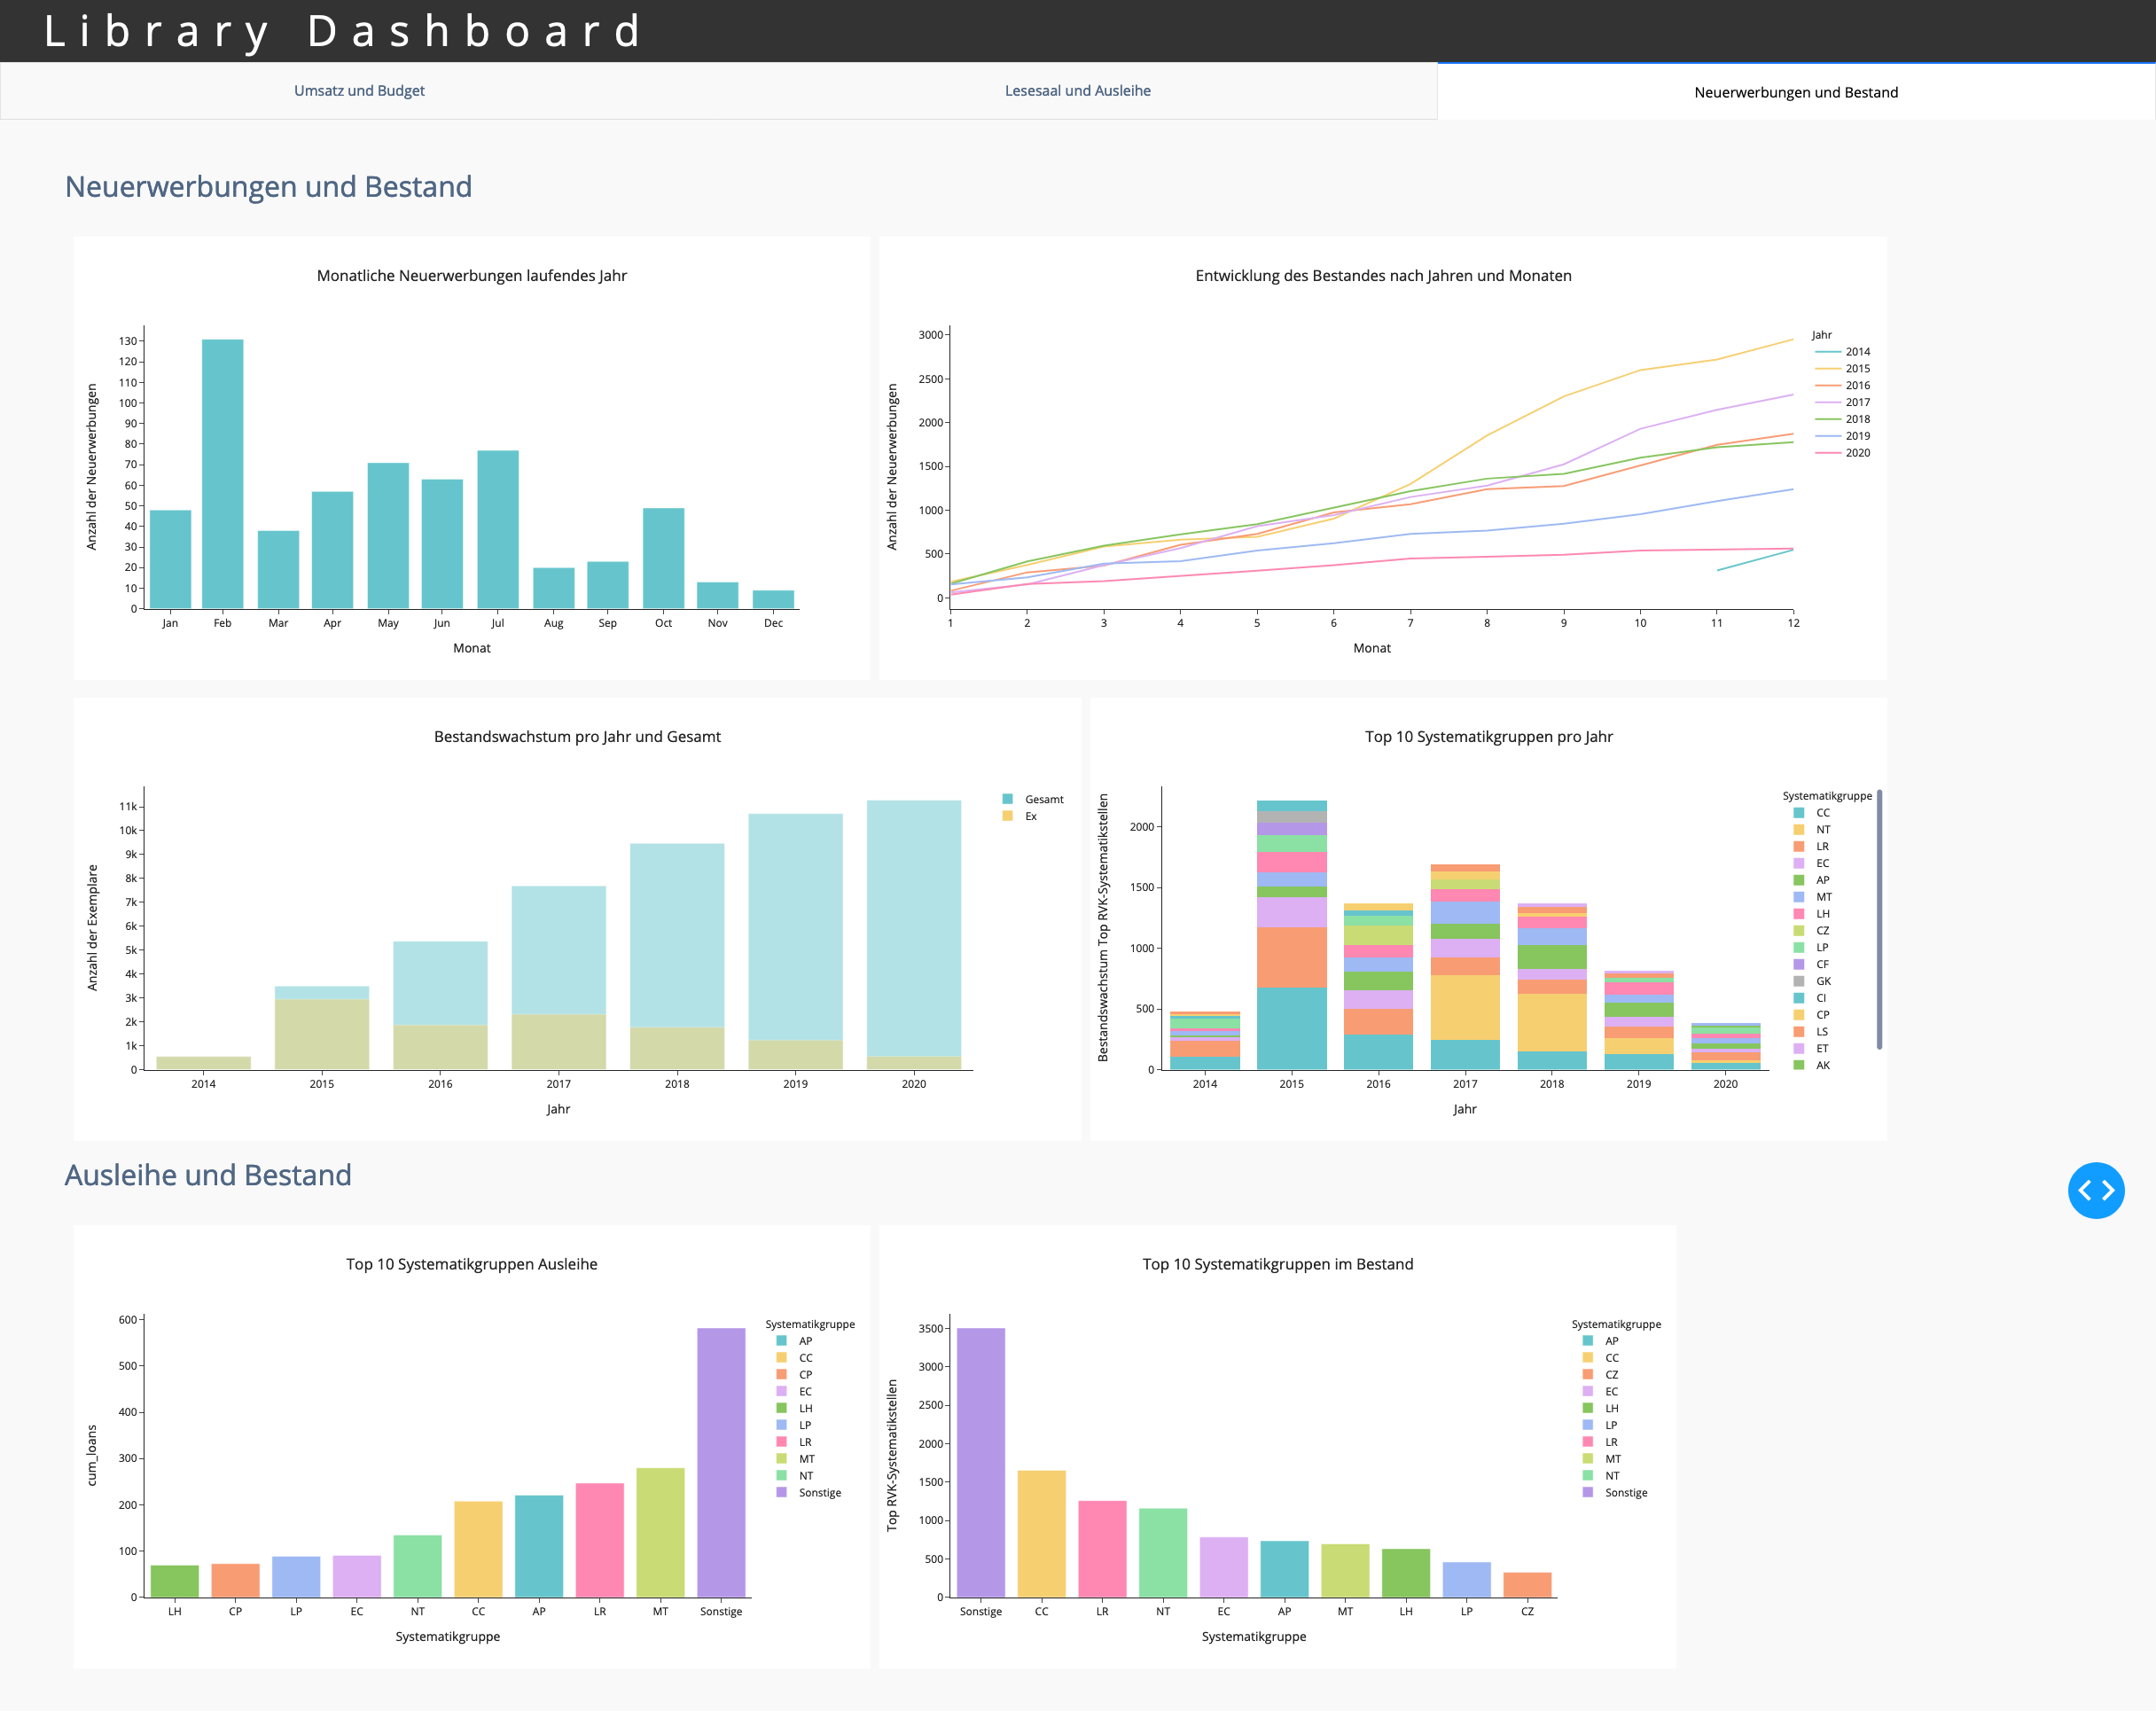
\includegraphics[width=22cm, height=26cm]{tab3}
            \caption{Tab3}
            \label{fig:tab3}
    \end{figure}

    %\clearpage
    \KOMAoptions{paper=A4,paper=portrait}
    \recalctypearea 
    %Folgende Diagramme werden im Tab \textit{Neuerwerbungen und Bestand} dargestellt.
    \begingroup
    \setlength{\tabcolsep}{12pt} % Default value: 6pt
    \renewcommand{\arraystretch}{1.0} 
    \begin{table}[H]
        \LARGE
        \centering
        \begin{adjustbox}{max width=\textwidth}
        \begin{tabular}{p{0.1\textwidth}p{0.5\textwidth}p{0.4\textwidth}p{0.3\textwidth}p{0.4\textwidth}p{0.4\textwidth}}
           \toprule
           Row        &Titel der Darstellungen&Beschreibung &Datenset &Darstellung &Interaktivität auf dem Dashboard\\
           \midrule
            1           &Monatliche Neuerwerbungen laufendes Jahr&Es werden die monatlichen Neuerwerbungen des laufenden Jahres dargestellt.&Bestandsdaten&Balkendiagramm&-\\
                        &Jährliche Bestandsentwicklung nach Monaten&Darstellung des akkumulierten Bestandswachstums für die einzelnen Jahre&Bestandsdaten&Liniendiagramm    &Plotly-Interaktivität (Aus- und Einblenden von Linien, Hover-Informationen)\\          
            \midrule
            2           &Bestandswachstum pro Jahr und Gesamt&Darstellung des absoluten und des relativen Wachstums nach Jahren.&Bestandsdaten&überlagertes Balkendiagramm&Plotly-Interaktivität (Aus- und Einblenden von Balken, Hover-Informationen)\\
                        &Top 10 RVK-Fachsyste-matiken pro Jahr&Die jährlichen Top 10 \textit{\acrshort{RVK}}-Fachsys-tematiken im Bestand werden dargestellt.&Bestandsdaten    &gestapeltes Balkendiagramm&Plotly-Interaktivität (Aus- und Einblenden von Balken, Hover-Informationen)\\
            \midrule
            3           &Top RVK-Fachsystema-tiken Ausleihe mit Sonstige&Es werden 9 \textit{\acrshort{RVK}}-Fachsyste-matiken der Ausleihe vom kleinsten Wert zum größten des Bestandes (ohne Buchservice) dargestellt. Die übrigen Systematiken werden in Sonstige dargestellt.&Ausleihdaten&Balkendiagramm&Plotly-Interaktivität (Aus- und Einblenden von Balken, Hover-Informationen)\\
                        &Top RVK-Fachsystema-tiken Bestand mit Sonstige&Es werden  9 \textit{\acrshort{RVK}}-Fachsyste-matiken im Bestand vom größten Wert zum kleinsten dargestellt. Die übrigen Systematiken werden in Sonstige dargestellt.&Bestandsdaten&Balkendiagramm&Plotly-Interaktivität (Aus- und Einblenden von Balken, Hover-Informationen)\\

        \bottomrule
        \end{tabular}
        \end{adjustbox}
        \caption
        \end{table}
    \endgroup

\section{Bewertung}

\subsection{Allgemeines}
\label{chap:five_three_one}
Das Ziel des vorliegenden Projektes war es, ein Proof-of-Concept eines Systems zu entwickeln, 
das wesentliche bibliothekarische Daten sammelt, statistisch mit geeigneten Methoden und
Datenvisualisierungen analysiert. Als Ergebnis steht ein datengetriebenes 
Unterstützungssystem, das durch drei Teilsysteme den Import und eine erste Bereinigung der Daten,
die Aufbereitung der Daten, die Umwandlung der Daten in Datenvisualisierungen und deren Darstellung garantiert. 
Das System verarbeitet bibliothekarische Daten aus den Bereichen Umsatz und Budget, Lesesaal und Ausleihe 
sowie der Bestandsentwicklung. Es wurde vor dem Hintergrund der regelmäßigen Datenbereitstellung entwickelt.

Das System ist ausgelegt auf diese bibliothekarischen Daten, die aus heterogenen Datenquellen stammen.
Diese Daten bringen spezifische Anforderungen wie Datenbeschaffenheit oder Dateiformatspezifikationen mit, 
die den Prozess der Datenintegration in das System bestimmen. Es konnte mit dem System gezeigt werden, 
dass diese Anforderungen für die vorliegenden Daten vom System erfüllt wurden, indem entsprechende Prozesse innerhalb
der drei Teilsysteme für diese Daten entwickelt wurden.

So erwartet das System beim Import die Daten in einer gewissen Struktur (Datenformat). 
Überdies muss das Dateiformat dem System bekannt sein und der Dateiname speziellen semantischen 
Kriterien entsprechen. Wenn diese Anforderungen erfüllt sind, können die Daten problemlos in das System integriert werden.
Weiterhin können bestimmte Modifikationen eingestellt werden wie die Entfernung
bestimmter Zeichen im Teilsystem 1. Diese Modifikationen sind aber sehr einfach und wurden aus der Voranalyse
der Daten entwickelt. Die Modifikationen können zwar auf andere Daten angewendet werden, gelten aber ersteinmal nur für die vorliegenden Daten. 
Darüberhinaus bietet das System im Teilsystem 1 keine weiteren einstellbaren Möglichkeiten an. Ferner ist das System auf einfache 
Tabellenstrukturen, wie sie in tsv- oder Excel-Dateien abgespeichert werden können, ausgerichtet.
Grundsätzlich erfolgt der Import der Daten (einfache Tabellenstrukturen) aus heterogenen Datenquellen 
in einfache Tabellenstrukturen in einem einheitlichen csv-Dateiformat. Der einfache Import von Daten von einem Dateiformat 
in das csv-Format ist aber problemlos möglich, wenn Daten vorliegen, die keine weiteren speziellen
Anforderungen besitzen.

Das Teilsystem 2 und das Teilsystem 3 erwarten csv-Dateien, die sie weiterverarbeiten können. 
Deshalb kann das System auch unabhängig vom Teilsystem 1 funktionieren. 
Das Teilsystem 1 stellt vielmehr eine Möglichkeit dar, wie der Import der Daten ablaufen kann. 
Das Teilsystem 1 wurde für das System entwickelt, da insbesondere mit den vorliegenden Daten umgegangen werden musste und ebenfalls hier 
der Großteil der Datenanreicherung abläuft.


\subsection{Datenlage im vorliegendem System}
In dem vorliegenden Projekt wurden hauptsächlich die heterogenen Bibliotheksdaten aus dem \textit{\acrshort{hebis}}-Verbund sowie aus dem \textit{\acrlong{LBS}} Frankfurt verarbeitet.
Da potentiell alle Bibliotheken, die durch das \textit{\acrshort{LBS}}-Team Frankfurt betreut werden, die gleichen Daten zur Verfügung gestellt bekommen,
kann das vorliegende  System von diesen Bibliotheken implementiert werden. Eine Aussage darüber, ob es in anderen Bibliotheken oder Verbünden implementiert werden kann, die ebenfalls
Instanzen des \textit{\acrlong{CBS}s} und \textit{\acrshort{LBS}} betreiben, kann leider hier nicht getroffen werden, da die technische Infrastruktur
und die Datenbereitstellung stark differieren können. 

Der Workflow für den Import, die Weiterverarbeitung und die Darstellung der Umsatz- und Budgetdaten sowie der Bestandsdaten kann durch das System
abgedeckt werden, da die hierfür benötigten Daten der Bibliothek regelmäßig zur Verfügung gestellt werden. Die Ausleihdaten werden nicht automatisch
geliefert. Dadurch entsteht eine Schieflage zwischen Bestands- und Ausleihdaten in Bezug auf die Bestandsgröße.
Deshalb müssten im Regelbetrieb sowohl die bibliotheksinternen Prozesse und als auch das System angepasst werden, um einen regelmäßigen Abzug der Ausleihdaten
verarbeiten zu können. Zur Zeit ist das System auf die vorliegenden Ausleihdaten zugeschnitten.

% Data is messy - Library data too!
Teilweise mussten die Daten aufgrund von Unzulänglichkeiten angepasst und bearbeitet werden.
Zu nennen wären hier fehlende Daten in den Umsatz- und Budgetdaten. Diese fehlenden Daten können Fehler in der Darstellung im Dashboard erzeugen.\footnote{Ebenso fehlen noch relevante Lieferanten, die sich nicht im \textit{\acrshort{LBS}} finden lassen.}
Des Weiteren werden bei dem monatlichen Abzug der Neuerwerbungsdaten aus dem \textit{\acrshort{CBS}} Duplikate mit exportiert. Diese Duplikate entstehen durch
Mehrfachexemplare, die an einem Datensatz hängen. Diese lassen sich zwar als Duplikate relativ einfach über die Signatur erkennen und entfernen.
Darunter würden dann aber auch alle ebooks fallen, da sie die gleiche Signatur aufweisen. Mit diesen Ausnahmen innerhalb der Daten musste und wurde ein Umgang gefunden. Diese haben mitunter alle Teilsysteme affektiert und
die Programmierung dieser mitbestimmt.

In Bezug auf die Darstellung der Daten im Dashboard stellt die Vielzahl von diskreten Werten ein Problem dar. 
Die Grenze der Darstellbarkeit der Daten in Form von Diagrammen ist erreicht, wenn zu viele diskrete Werte dargestellt werden müssen.
Das betrifft zum Beispiel die Vielzahl an Lieferanten in dem Diagramm \enquote{Gesamtumsatz Lieferanten nach Jahren} im Tab \textit{Umsatz und Budget}. 
Dort kann anhand der Farbe in den gestapelten Balkendiagramm nicht mehr zwischen den einzelnen Lieferanten unterschieden werden, da die Color-Palette 
nur eine bestimmte Anzahl an diskreten Werten darstellen kann \cite[vgl.][]{plotly_discrete_2021}.\footnote{Auch wäre die Frage zu stellen, inwieweit hier die Darstellung aller Lieferanten 
überhaupt sinnvoll ist im Hinblick auf die Informationsrezeption.}
Ebenso betrifft dieses Problem die Auswertung der Bestandsdaten nach den \textit{\acrshort{RVK}}-Fachsystematiken beziehungsweise nach deren Untergruppen. 
Erste Datenanalysen haben verdeutlicht, dass es eine große Vielzahl an Fachsystematiken im Bestand der Bibliothek gibt, sodass eine visuelle Darstellung aller Fachsystematiken nicht zielführend ist.
Aufgrund dieser Darstellungsprobleme bei den Umsatz- und Besandsdaten wurden zusätzlich noch andere Diagramme erstellt, die die Anzahl der darzustellenden Werte durch bestimmte Clusterungen reduziert.
So wurde ein Diagramm erstellt, das eine bestimmte Anzahl der umsatzstärksten Lieferanten im Gesamtzeitraum zeigt. Bei den \textit{\acrshort{RVK}}-Fachsystematiken wurde ebenso
verfahren.



\subsection{Umgesetzte Anforderungen der Anforderungsanalyse}
Im Folgenden wird sich auf die Muss-Anforderungen der Anforderungsanalyse konzentriert, die durch das Proof-of-Concept
umgesetzt werden sollten. Dabei werden die Rahmenbedingungen, die funktionalen sowie die nicht-funktionalen Anforderungen
betrachtet.
%Dennoch können die Diagramme im Frontend schon jetzt in einem plazsparenden Bildformat gespeichert werden durch die Bereitsellung einer Ploly-Funkion.

Im Bereich des \textit{\acrshort{ETL}}-Prozesses und der Datenspeicherung (\autoref{tab:funktionale Anforderungen I}) wurden die Anforderungen F1, F2, F4, und F5 erfüllt.
% Das Parsen der unterschiedlichen Dateiformate geschieht durch verschiedene pandas-Funktionen, die die Datentypen der Werte
% aus den vorliegenden Werten in den Spalten automatisch ableiten. Das klappte für das vorliegende Projekt sehr gut, dass
% bei diesem Prozess nicht manuell eingegriffen wurde.
Die Anforderung F3 musste nicht umgesetzt werden, da die Daten bereits so vorlagen, dass auf ihnen ohne automatische Harmonisierung weitergearbeitet werden konnte.
Bedingt wurde dennoch diese Anforderung durch die Datenanreicherung abgedeckt. Auch durch das Speichern im Utf-8-Zeichenformat konnte hier bereits eine Harmonisierung der
Zeichenkodierung erzielt werden.

Die funktionalen Anforderungen der Datenanalyse (\autoref{tab:funktionale Anforderungen II}) wurden vollständig erfüllt (F10 - F14).
Die funktionalen Anforderungen F15 und F16 des Bereiches Datenpräsentation und Standardbericht (\autoref{tab:funktionale Anforderungen III}) 
wurden ebenso erfüllt. Es gibt eine Vielzahl an Datenvisualisierungen, die den Benutzer:innen auf dem Dashboard angeboten werden. 
Diese bestehen neben Kreisdiagrammen und einer Tabelle hauptsächlich aus Linien- und Balkendiagrammen.
Die Erzeugung des Standardberichts wurde nicht mehr implementiert. Dementsprechend wurden die diesbezüglichen
Anforderungen (F18, F20, F21) nicht umgesetzt. 

Von den nicht-funktionalen Anforderungen (\autoref{tab: nfAnforderungen}) wurden folgende erfüllt:\\
NF1, NF5, NF6, NF8, NF11, NF12, NF15, NF16, NF17, NF18. 
Da das System nur ein Proof-of-Concept darstellt, wurde es noch nicht anderen
Benutzer:innen vorgestellt, deswegen kann die Anforderung NF2 \enquote{Das System ist leicht erlernbar} noch nicht als erfüllt gelten.

Die Grenze der Darstellbarkeit in Diagrammen betrifft die Umsetzung der nicht-funk-tionalen Anforderung NF14 \enquote{Die verschiedenen Diagrammtypen werden zielgerichtet eingesetzt}
die nicht vollständig realisiert werden konnte. Da nur eine bestimmte Anzahl an Werten übersichtlich präsentiert werden kann, gilt es die Auswahl der Diagramme
beziehungsweise der in ihnen dargestellten Daten zu evaluieren. 



\subsection{Umgesetzte Anwendungsfälle}
Die Anwendungsfälle 1, 3, 4, 5, 6 wurden bearbeitet und umgesetzt.
Die Anwendungsfälle 2 und 7 konnten im Projektzeitrahmen nicht mehr bearbeitet werden, 
da die Zeit nicht mehr ausgereicht hat. Gründe hierfür waren unter anderem eine komplexere Tabellenstruktur (Anwendungsfall 2),
die vermutlich erst in einfachere Strukturen aufgelöst hätte werden müssen. Im Folgenden wird das Systemverhalten für jeden
Anwendungsfall tabellarisch dargestellt.\\

\clearpage
\noindent
\textit{Anwendungsfall 1}\\
% Titel: Ausleihzahlen Bibliotheksbestand\\
Das Ziel des \textit{Anwendungsfall 1} ist die Darstellung der Anzahl der Ausleihen des Bestandes.
Die Ergebnisse befinden sich in dem\textit{Tab2 - Lesesaal und Ausleihe} des Dashboards.

\begingroup
    \setlength{\tabcolsep}{12pt} % Default value: 6pt
    \renewcommand{\arraystretch}{1.5} 
    \begin{table}[h]
        \Large
        \centering
        \begin{adjustbox}{max width=\textwidth}
        \begin{tabular}{p{0.4\textwidth}p{0.5\textwidth}p{0.7\textwidth}}
           \toprule
           Systemverhalten        &Titel der Darstellungen&Bemerkung\\
           \midrule
           Das System filtert die betreffenden Datensätze nach Jahr. Das System zeigt diese Datensätze mit Datenvisualisierungen an.&-&Durch die Teilsysteme 2  und 3 gewährleistet.\\
           Das System zeigt die ausleihstärksten Titel absteigend nach Anzahl und aufsteigend nach Jahr an.&Tabellarische Darstellung der 5 besonders nachgefragten Titel nach Jahren&Die Anzahl der anzuzeigenden Titel kann im Programmcode der Datei \texttt{loan\_read\_tab.py} beim Methodenaufruf als Parameter eingestellt werden.\\
           Das System zeigt die Verteilung der ausgeliehenen Titel nach \textit{\acrshort{RVK}}-Fachsys-tematiken pro Jahr an.&Ausleihe Top RVK-Fachsystematiken mit Buchservice und Sonstige&Die Anzahl der \textit{\acrshort{RVK}}-Fachsystematiken kann im Programmcode der Datei \texttt{loan\_read\_tab.py} beim Methodenaufruf als Parameter eingestellt werden.\\
           Das System zeigt die Top-\textit{\acrshort{RVK}}-Fachsys-tematiken der Ausleihe an.&Ausleihe Top RVK-Fach-systematiken pro Jahr\footnotemark&Die Anzahl der \textit{\acrshort{RVK}}-Fachsystematiken kann im Programmcode der Datei \texttt{loan\_read\_tab.py}beim Methodenaufruf als Parameter eingestellt werden.\\
           Das System zeigt die Verteilung der Ausleihe unterschieden in Bibliotheksbestand und Buchservice an.&Gesamtverteilung Ausleihe Buchservice / Bibliothek&-\\
        \bottomrule
        \end{tabular}
        \end{adjustbox}
        \caption
        \end{table}

    \footnotetext{Ein weiteres Diagramm zu den Top-\textit{\acrshort{RVK}}-Fachsystematiken der Ausleihe (ohne dem Buchservice) befindet sich in dem Dashboard Tab \textit{Neuerwerbungen und Bestand} zur verständlicheren Gegenüberstellung zu den Bestandsdaten.}

    \endgroup

\clearpage
\noindent
\textit{Anwendungsfall 3}\\
% Titel: Lesesaalnutzung\\
Das Ziel des \textit{Anwendungsfall 3} ist die Anzeige der Nutzung des Lesesaals während der Öffnungszeiten.
Die Ergebnisse befinden sich in dem\textit{Tab2 - Lesesaal und Ausleihe} des Dashboards.

\begingroup
    \setlength{\tabcolsep}{12pt} % Default value: 6pt
    \renewcommand{\arraystretch}{1.5}
    \begin{table}[h]
        \Large
        \centering
        \begin{adjustbox}{max width=\textwidth}
        \begin{tabular}{p{0.4\textwidth}p{0.5\textwidth}p{0.7\textwidth}}
           \toprule
           Systemverhalten        &Titel der Darstellungen&Bemerkung\\
           \midrule
           Das System filtert die betreffenden Datensätze nach Jahr. Das System zeigt diese Datensätze mit Datenvisualisierungen an.&-&Durch die Teilsysteme 2  und 3 gewährleistet.\\
           Das System zeigt die Nutzung des Lesesaals nach Monat und Jahr, gruppiert in vier Service-Zeiten an.&Monatliche Anzahl der Nutzer:innen nach Service-Zeiten, Jährliche Lesesaalnutzung nach Service-Zeiten& Die Jahre können im Dropdown-Menü im Dashboard ausgewählt werden.\\

        \bottomrule
        \end{tabular}
        \end{adjustbox}
        \caption
        \end{table}
\endgroup

\clearpage
\noindent
\textit{Anwendungsfall 4}\\
% Titel: Neuerwerbungen\\
Das Ziel des \textit{Anwendungsfall 4} ist die Anzeige der Anzahl der Neuerwerbungen pro Monat.
Die Ergebnisse befinden sich in dem \textit{Tab3 - Neuerwerbungen und Bestand} des Dashboards.

\begingroup
    \setlength{\tabcolsep}{12pt} % Default value: 6pt
    \renewcommand{\arraystretch}{1.5} 
    \begin{table}[h]
        \centering
        \Large
        \begin{adjustbox}{max width=\textwidth}
        \begin{tabular}{p{0.4\textwidth}p{0.5\textwidth}p{0.7\textwidth}}
           \toprule
           Systemverhalten        &Titel der Darstellungen&Bemerkung\\
           \midrule
           Das System filtert die betreffenden Datensätze. Das System zeigt diese Datensätze mit Datenvisualisierungen an.&-&Durch die Teilsysteme 2  und 3 gewährleistet.\\
           %Die Bibliotheksleitung und die Bibliotheksmitarbeiter:innen wählen einen Monat auf der \textit{\acrshort{GUI}} aus.&-&Diese Interaktion wurde nicht zusätzlich implementiert, da die Darstellung durch die zwei anderen Diagramme als genügend betrachtet wurde.\\
           Das System zeigt die Neuerwerbungen des laufenden Jahres an.&Monatliche Neuerwerbungen laufendes Jahr&-\\
           Das System zeigt die jährliche Bestandsentwicklung pro Monat an.&Jährliche Bestandsentwicklung nach Monaten&Der Verlauf der Bestandsentwicklung der einzelnen Jahre wird akkummuliert angezeigt.\\
           Das System zeigt die Anzahl der Titel nach Medienart an.&-&Diese Anforderung wurde zwar im Programmcode implementiert, aber nicht im Dashboard umgesetzt, da das gedruckte Buch als Medium sehr stark dominiert und in der Anzahl zu wenige andere Medienarten in der Bibliothek vertreten sind.\\

        \bottomrule
        \end{tabular}
        \end{adjustbox}
        \caption
        \end{table}
\endgroup

\clearpage
\noindent
\textit{Anwendungsfall 5}\\
% Titel: Bestandswachstum\\
Das Ziel des \textit{Anwendungsfall 5} ist die Anzeige Wachstums des Bibliotheksbestandes insgesamt und nach einzelnen \textit{\acrshort{RVK}}-Fachsystematiken.
Die Ergebnisse befinden sich in dem \textit{Tab3 - Neuerwerbungen und Bestand} des Dashboards.

\begingroup
    \setlength{\tabcolsep}{12pt} % Default value: 6pt
    \renewcommand{\arraystretch}{1.5} 
    \begin{table}[h]
        \centering
        \Large
        \begin{adjustbox}{max width=\textwidth}
        \begin{tabular}{p{0.4\textwidth}p{0.5\textwidth}p{0.7\textwidth}}
           \toprule
           Systemverhalten       &Titel der Darstellungen&Bemerkung\\
           \midrule
           Das System filtert die betreffenden Datensätze. Das System zeigt diese Datensätze mit Datenvisualisierungen an.&-&Durch die Teilsysteme 2 und 3 gewährleistet.\\
           Das System zeigt die Top-\textit{\acrshort{RVK}}-Fachsyste-matiken des Bestandes pro Jahr an.&Top 10 RVK-Fachsyste-matiken pro Jahr&Die Anzahl der Fachsystematiken kann im Programmcode der Datei \texttt{newacq\_coll\_tab.py} beim Methodenaufruf als Parameter eingestellt werden.\\
           Das System zeigt die Gesamtzahl der Titel nach Jahren an.&Bestandswachstum pro Jahr und Gesamt&-\\
           Das System zeigt die Anzahl der Titel nach Medienart an.&-&Diese Anforderung wurde zwar im Teilsystem 2 implementiert, aber wird nicht als Diagramm im Dashboard gezeigt, da das gedruckte Buch als Medium sehr stark dominiert und in der Anzahl zu wenige andere Medienarten in der Bibliothek vertreten sind.\\
           Das System zeigt die Top-\textit{\acrshort{RVK}}-Fachsyste-matiken des Bestandes insgesamt an.&Top RVK-Fachsystema-tiken Bestand mit Sonstige&Die Anzahl der Fachsystematiken kann im Programmcode der Datei \texttt{newacq\_coll\_tab.py} beim Methodenaufruf als Parameter eingestellt werden.\\
        \bottomrule
        \end{tabular}
        \end{adjustbox}
        \caption
        \end{table}
\endgroup

\clearpage
\noindent
\textit{Anwendungsfall 6}\\
% Titel: Umsatz- und Budgetübersicht\\
Das Ziel des \textit{Anwendungsfall 6} ist die Anzeige der Umsatz- und Budgetübersicht für den Gesamtzeitraum und das laufende Jahr.
Die Ergebnisse befinden sich in dem \textit{Tab1 - Umsatz und Budget} des Dashboards.

\begingroup
    \setlength{\tabcolsep}{12pt} % Default value: 6pt 
    \renewcommand{\arraystretch}{1.5} 
    \begin{table}[h]
        \centering
        \Large
        \begin{adjustbox}{max width=\textwidth}
        \begin{tabular}{p{0.4\textwidth}p{0.5\textwidth}p{0.7\textwidth}}
           \toprule
           Systemverhalten        &Titel der Darstellungen&Bemerkung\\
           \midrule
           Das System filtert die betreffenden Datensätze. Das System zeigt diese Datensätze mit Datenvisualisierungen an.&-&Durch die Teilsysteme 2 und 3 gewährleistet.\\
           %Die Bibliotheksleitung und die Bibliotheksmitarbeiter:innen können sich den Lieferanten auswählen und den Gesamtumsatz und den Umsatz pro Jahr ansehen.&Gesamtumsatz Lieferant nach Jahren, Gesamtumsatz Lieferant nach Jahren, Lieferant Umsatz pro Monat laufendes Jahr&Die einzelnen Lieferanten können im Dropdown-Menü im Frontend ausgewählt werden.\\
           Das System zeigt den Umsatz im laufenden Jahr und den Jahresdurchschnittsumsatz eines Lieferanten.&Umsatz laufendes Jahr (für einen Lieferanten), Jahresdurchschnitt (Lieferant)&Die einzelnen Lieferanten können im Dropdown-Menü im Dashboard ausgewählt werden.\\
           Das System zeigt die umsatzstärksten Lieferanten im Gesamtzeitraum an.&Top 10 Lieferanten mit Sonstige  &Die Anzahl der Lieferanten kann im Programmcode der Datei \texttt{expenditures\_tab.py} beim Methodenaufruf als Parameter eingestellt werden.\\
           Das System zeigt den Gesamtumsatz im Gesamtzeitraum und im laufenden Jahr&Gesamtumsatz Lieferanten nach Jahren, Gesamtumsatz, Gesamtumsatz laufendes Jahr&-\\
           %Die Bibliotheksleitung und die Bibliotheksmitarbeiter:innen können sich die Budgetübersicht ansehen.&Gesamtbudget Kostenstellen nach Jahren&-\\
           Das System zeigt das Budget über den Gesamtzeitraum pro Kostenstelle an.&Top 5 Kostenstellen mit Sonstige, Gesamtbudget Kostenstellen nach Jahren&-\\
           Das System zeigt die kostenintensivsten Kostenstellen im Gesamtzeitraum an.&Top 5 Kostenstellen mit Sonstige&Die Anzahl der Kostenstellen kann im Programmcode der Datei \texttt{expenditures\_tab.py} beim Methodenaufruf als Parameter eingestellt werden.\\
        \bottomrule
        \end{tabular}
        \end{adjustbox}
        \caption
        \end{table}
\endgroup
\clearpage
    \subsection{Erweiterbarkeit des Systems}
    Wie in \autoref{chap:five_three_one} dargelegt wurde, erwartet das datengetriebene Unterstützungssystem bestimmte Daten,
    damit es problemlos läuft. Die Integration neuer Datenquellen ist mit dem System prinzipiell möglich. 
    Jedoch, je heterogener die Datenquellen und je heterogener die Daten selbst beschaffen sind, 
    desto größer ist der Aufwand, diese in das System zu integrieren. Bei der Integration neuer Daten in 
    das System müsste das Teilsystem 2 und auf jeden Fall das Teilsystem 3 erweitert werden.
    Entweder werden Klassen/Methoden des Programmcodes des Teilsystems 2 nachgenutzt oder es 
    müssen Klassen/Methoden im Teilsystem 2 neu geschrieben werden. Da das Erstellen der Diagramme gleichfalls auf die vorliegenden 
    Daten konkret zugeschnitten ist, muss ebenfalls die Logik für die Diagramme und für deren Darstellung im Dashboard
    neu implementiert werden. Das kann mitunter sehr aufwendig sein. Ob diese neuen Daten mit dem Teilsystem 1 bearbeitet
    werden müssen oder ob sie unabhängig davon bereitgestellt werden, hängt von den Spezifikationen der Daten und dem
    Dateiformat ab. Der Verzicht auf das Teilsystem 1 wäre möglich.

    Das System bietet momentan kein Baukastenset aus verschiedenen Methoden zur Auswertung 
    und Datenvisualisierung an, das für die einzelnen Daten nur noch zusammengesetzt
    werden müsste. Für neue Datenauswertungen oder für neue Darstellungen durch Datenvisualisierungen 
    im Dashboard müssen die Teilsysteme 2 und 3 erweitert werden. In Abhängigkeit von den Aspekten, nach denen
    die Daten ausgewertet werden, oder welche Datenvisualisierung zum Einsatz kommen sollen,
    berechnet sich der Aufwand für die Anpassung des Systems. 
    Wie stark das System erweitert werden muss, hängt aber auch von der Beschaffenheit der Daten und deren Struktur ab. 
    Zum Beispiel ließen sich die Umsatz- und Budgetdaten aus der LBS-Datenbank leicht integrieren, da die Daten 
    in ihrer Struktur sehr ähnlich sind. Für andere Daten aus dieser Datenbank wäre es vorstellbar,
    dass die Integration der Daten ebenso leicht funktionieren würde. Für Daten aus anderen Quellen
    müssten wahrscheinlich Prozesse neu aufgesetzt werden, die alle Teilsysteme einschließen.


    Die Abhängigkeit von Datenlieferanten zieht immer auch eine Unsicherheit in der Frage der Datenkonsistenz
    nach sich. Veränderungen bei der Datengenerierung können zu Veränderungen in der inhaltlichen Datenstruktur führen und
    können für das vorliegende System Probleme aufwerfen.
    Diese Probleme können zu Fehlern in der Berechnung und der Darstellung der Daten führen. 
    Das vorliegende System steht solchen Änderungen blind gegenüber und müsste dementsprechend angepasst werden. 
    Die Anpassung an die neuen Datenstrukturen wird bestimmt durch den Grad der Schwere der Veränderung und kann alle Teilsysteme affektieren. 
    Wenn sich zum Beispiel die vorliegende Tabellenstruktur der zu importierenden Daten ändert, wie zum Beispiel 
    durch das Hinzukommen neuer Informationen in neuen Spalten, kann das auch einen Einfluss haben 
    auf die Speicherdateien mit den bereits importierten Daten. Gegebenenfalls wäre die Datei so korrumpiert,
    dass sowohl die Datenauswertungen und die Datendarstellungen nicht mehr funktionieren. Die Behebung dieses Problems 
    würde vermutlich einen hohen zeitlichen Aufwand nach sich ziehen. Zudem würde es die Frage aufwerfen, 
    ob der informationsverlustfreie Import, der durch das Teilsystem 1 angestrebt wird, aufrecht erhalten werden sollte.
    Hier wäre einerseits zu überlegen, ob nur diejenigen Daten mitimportiert werden, die wichtig für die Auswertung
    und Darstellung wichtig sind. Das heißt, das die Anforderungen bezüglich der Auswertungen vorher bekannt sein müssen und
    nicht ad hoc erweitert werden können.
 
  
\chapter{Fazit und Ausblick}
\label{chap:six}
Das Ziel, ein System für die Budgetplanung und Mittelallokation zu entwickeln, an dem die
Bibliotheksleitung und die Mitarbeiter:innen relevante \textit{\acrlong{KPI}} wie Umsatz- und Budgetübersichten, Ausleihzahlen und Bestandsinformationen ablesen
können, ist durch das vorliegende Proof-of-Concept umgesetzt wurden. Das System aggregiert relevante Daten, die statistisch mit geeigneten und
modernen Datenvisualisierungen analysiert werden.

Das datengetriebene Unterstützungssystem, das in dieser Arbeit konzeptionell entworfen wurde, erfüllt drei Hauptaufgaben:
den Import von bibliothekarischen Daten aus heterogenen Datenquellen in ein einheitliches Dateiformat, die Auswertung der Daten mit deskriptiven Methoden der Statistik
wie die Darstellung der Lagemaße oder mit Visualisierungen der Daten in einem Dashboard.
Dieses System funktioniert für die vorliegenden bibliothekarischen Daten gut.

Für die Beschaffung der bibliothekarischen Daten gibt es in der Bibliothek bereits Prozesse, auf die bei der Umsetzung des Proof-of-Concepts 
zurückgegriffen werden konnte. So werden die Umsatz- und Budgetdaten seit 2018 regelmäßig jeden Monat vom \textit{\acrshort{LBS}}-Team geliefert. Die benötigten Daten für die 
Jahre 2014 bis 2017 konnten - in einem anderen Format - unproblematisch vom \textit{\acrshort{LBS}}-Team nachgeliefert werden. Um die Daten für den Import passend zu machen, 
musste hier manuell trotzdem nochmal nachgebessert werden. Problematisch war die Datenbasis für die monatlichen Neuerwerbungen. Die Neuerwerbungsdaten wurden 
in der Vergangenheit nur sehr unregelmäßig aus dem \textit{\acrshort{CBS}} abgezogen, so dass dieser Datenbestand viele Lücken aufwies. Leider war es in Verbindung mit den Neuerwerbungen 
ebenfalls nicht möglich, einen gesamten Abzug des Bestandes für das datengetriebene Unterstützungssystem zu nutzen, da die wichtige Datuminformation für die 
Neuerwerbungen in dem Abzug fehlte. So wurden die Daten für den Zeitraum ab 2014 nochmals für jeden Monat aus dem \textit{\acrshort{CBS}} abgezogen. 



Vorkenntnisse der Daten existierten bereits aus früheren Auswertungen mit einem Tabellenkalkulationsprogramm, sodass eine solide Wissensbasis 
der einzelnen Daten bereits bestand. Dennoch wurde der Aufwand des gründlichen Sichtens der Daten unterschätzt, so dass bei 
der Implementation des Systems und der Arbeit mit den Daten Probleme auftraten. 
Problematisch war dies insbesondere bei den Ausleihdaten. Durch die Validierung der RFID-Etiketten in
den Medien am Selbstverbucher durch die Bibliothek wird eine größere Anzahl an Ausleihen erzeugt als eigentlich ausgeliehen wird. 
Dagegen wurde mit einer Programmmethode beim Import der Ausleihrohdaten vorgegangen, die unabhängig (unbedacht) von den Jahrensangaben in den Daten die Ausleihanzahl der Medien um eins reduzierte. 
So kann es sein, dass ein Medium in fünf Jahren jeweils einmal ausgeliehen wurde, in den betreffenden Diagrammen aber überhaupt nicht erscheint. 
Hier gilt es die Methode im Programmcode zu erweitern, sodass die Jahresangabe in den Daten mit berücksichtigt werden kann. Darüberhinaus ist die konkrete bibliothekarische Praxis der Medienerschließung zu überdenken.
Wegen solcher Probleme, sollte der zeitliche Aufwand der Voranalyse der Daten in Hinsicht auf die Integration neuer
Daten in das System, nicht unterschätzt werden und ihr einen größtmöglichen Platz eingeräumt werden. 

Das bibliothekarischen Domänwissen in Bezug auf das Datenformat der Titel- und Lokaldaten konnte
für die Bestands- und Neuerwerbungsdaten zielführend eingesetzt werden. Unbekannte Statistiken wie die \acrlong{COP 5} mussten aufgrund des engen Projektzeitplans leider unberührt bleiben.
Eine erste Überlegung, nur mit Daten zu arbeiten, die schon in dem für das System bevorzugten CSV-Format vorlagen, 
zerschlug sich an der Heterogenität der Datenmodelle. Auch waren Versuche, von vornherein die Daten in dem CSV-Format abzubilden, nicht zufriedenstellend.
Für die Transformation wurde daraufhin das Teilsystem 1 entwickelt.
Aufgrund des Rückgriffs auf die pandas Bibliothek, die viele Funktionen für die verschiedenen Dateiformate anbietet, konnte der Import aber sichergestellt werden.
% bibliothekarisches Domainwissen

Aus der Voranalyse der Daten und aus früheren Datenauswertungen wurden dann die Anforderungen und die Anwendungsfälle abgeleitet.
Diese wurden vor dem Beginn der Systemprogrammierung formuliert. In einem iterativen Entwicklungprozess wurden die Anforderungen und Anwendungsfälle kontinuierlich re-evaluiert und 
entsprechend angepasst. Leider war dies aufgrund des engen Zeitrahmens des Projekts nicht immer in vollem Umfang möglich. So wurden die Teilsysteme nacheinander entwickelt und
erst am Ende dieses Entwicklungsprozesses wurde das erwünschte Ergebnis in Form des Dashboards schließlich sichtbar. Vermutlich wäre es für den Verlauf der Systementwicklung sowie einer
Re-Evaluierung der Anforderungen und Anwendungsfälle besser gewesen, das System zunächst lediglich mit den Daten aus nur einem der vier bibliothekarischen Bereiche
aufzubauen. Danach hätte das System für die Daten aus den anderen Bereichen sukzessive erweitert werden können. 
So hätte man wahrscheinlich eine größere Chance gehabt, Fehler, die während der Systemprogrammierung entstanden und gelöst werden mussten, zu vermeiden.

% automatische Prozesse gegenüber manuelle Prozesse

% an unbekannte Daten wie Cop5 Statistiken nicht rangegangen -> da hier der zeitliche Aufwand zu groß gewesen wäre (Wie sind die Daten aufgebaut, was beschreiben sie,
% wie vollständig sind sie)
% -> nicht machbar in der Zeit, obwohl der Bibliotheken in der MPG Bedarfe gibt -> Anschlussprojekt

% dem Ermitteln der Anforderungen;
% Zusammentreffen des Entwicklers und Bibliothekars in einer Person
% bibliothekarischer Backgrounw´d wichtig beim Erkennen der Daten -> hat Einfluss auf die Entwicklung
% Fehlertoleranz -> welche Daten für die Auswertung können vernachlässigt werden,  wie wichtig ist das mitnehmen aller daten -> hat Auswirkungen auf
% Translation zwischen den statistischen Auswertungen die die Bibliothek schon gemacht und denen die automatisch erfolgen sollen.
% die Anforderungen, Translaionsprozess zwischen Anforderungen und Entwicklung zu minimieren, d.h. aber auch konkrete Anforderungen schreiben
% iterative Prozess hat aufgrund des engen zeitplans nicht so gut geklappt.
% Da die Teilsysteme nacheinander entwickelt wurden, hat es einer etwas größeren Vorstellungskraft gebraucht, um sich zum Beispiel mit den
% Diagrammen vorzustellen, erst am Schluss der Entwiicklung etwas zu sehen war
% Eigentlich wäre jetzt nochmal der Zeitpunkt gekommen, die Anforderungen und die Anwendungsfälle anzupassen und

% dem Umgang mit den verschiedenen Arten von Heterogenität [1] usw.)

% Es konnte mit der vorliegenden Arbeit demonstriert werden, dass Daten aus heterogenen Datenquellen in einem Dashboard dargestellt werden können.
% Dabei wurde ein System entwickelt, dass vom Datenimport über die Datenvorbereitung 
% bis hin zur Darstellung der vorhandenen Daten gut funktioniert. 
Eine Weiterentwicklung des Systems ist denkbar und wünschenswert. 
Neben der noch ausstehenden Umsetzung der Anwendungsfälle 2 und 7 betrifft die Weiterentwicklung alle Teilsysteme der Systemarchitektur
sowie deren technische Implementation. Vorstellbar wäre eine striktere Trennung der Teilsysteme. 
So könnte die Datenanreicherung ausschließlich im Teilsystem 1 erfolgen. Zur Zeit geschieht diese im Teilsystem 1 und im Teilsystem 2. 
Ebenso wäre es denkbar, die Implementation des Dashboards und die Erstellung der Diagramme im Teilsystem 3 zu trennen und diese in jeweils einzelne Teilsysteme
aufzulösen. Dadurch würde die Wartbarkeit des dahinterliegenden Programmcodes erhöht und der Programmcode könnte modularer strukturiert werden.
Eine andere Möglichkeit in diesem Zusammenhang wäre, das Teilsystem 3 durch Lösungen wie \textit{Tableau} oder \textit{apache superset} zu ersetzen.
Diese erstellen Dashboard-Applikationen mit einem Baukastensystem und können die Daten in verschiedenen Dateiformaten erwarten.\footnote{ Inwieweit die Ersetzung des Teilsystems 3 in die anderen Teilsysteme eingreifen würde, kann
hier nicht diskutiert werden.}

Um die Aktualität der Daten und der Darstellung garantieren zu können, könnte der Import der bibliothekarischen Daten automatisch erfolgen. So könnte auf das manuelle
Anstoßen des Imports verzichtet werden. Stattdessen würden die Daten mit einem CronJob importiert werden. Dabei wäre es wichtig, die Ergebnisse des Import-Prozesses in einer log-Datei zu protokollieren. 
Diese Ergebnisse können Meldungen des Systems über die Anzahl der zu importierenden Datensätze, über den erfolgreichen Import oder auch Fehlermeldungen sein.
Für das Protokollieren würde sich die Python Standardbibliothek Logging anbieten \cite[vgl.][]{sajip_logging_2021}.

Eine Weiterentwicklung wäre die Integration zusätzlicher Daten in das System wie die der Dokumentenlieferdienste oder die Nutzungsdaten elektronischer Ressourcen wie Online-Zeitschriften. 
Sowohl die Dokumentenlieferdienste als auch die Bereitstellung der elektronischen Ressourcen sind wichtige Informationsdienstleistungen der Bibliothek. 
Deren Darstellung würde den Informationsmehrwert des Dashboards erhöhen.
% Bei der Darstellung der Daten in den Diagrammen sollte nachgebessert werden. So zum Beispiel könnten Spitzen in den Nutzungszahlen des Lesesaals herausgerechnet oder die
% Servicegruppen-Zeiten in den Lesesaal-Diagrammen in die richtigen Proportionen gesetzt werden.


Zudem wäre es möglich, genauere oder zusätzliche Analysen - wie dem Bereitstellen zusätzlicher Diagramme - auf den bereits vorhandenen Daten zu vollziehen, um deren Aussagekraft zu erhöhen.
Weitere Datenanalysen könnten nach zusätzlichen Aspekten oder durch fortgeschrittene statistische Methoden erfolgen. Als Beispiel wäre die Auswertung der Bestandsdaten nach den \textit{\acrshort{RVK}}-Benennungen
zu nennen. Auch der Zusammenhang zwischen Bestand und Ausleihe könnte in einer Datenvisualisierung zum Ausdruck gebracht werden.
Um den Entwicklungsverlauf der dargestellten Daten hervorzuheben, könnten Trendlinien zu den Diagrammen hinzugefügt werden. Zusätzlich könnten Prognosen
für die Zukunft aus den vorhandenen Daten berechnet und dargestellt werden. Diese Weiterentwicklungen wären insbesondere für die Umsatz-und Budgetdaten interessant.

% Die einzelnen Diagramme könnten ebenfalls überarbeitet werden. Die Größe der Diagramme müsste angepasst werden, um die Proportionen den angezeigten Zahlenbereichen anzugleichen. 
% Die Ausnahmebehandlung bei der Datenbearbeitung war eine Schwierigkeit, die im Laufe der Systementwicklung öfters aufkam. Diese Ausnahmen
% entstanden 



%Das Layout des Dashboards könnte ebenfalls überarbeitet werden. 
%Es müssten die Größe der Diagramme angepasst werden, um die Proportionen den angezeigten Zahlenbereichen anzugleichen.
Ferner wurden im datengetriebenen Unterstützungssystem die mitgelieferten Funktionalitäten von Plotly Express nicht zur Gänze ausgeschöpft.
Hier bedarf es noch diverser Feineinstellungen für das Layoutverhalten der Diagramme.
Diese Anpassungen beziehen sich zum Beispiel auf die Legenden oder die Hover-Informationen.
Denkbar und sicherlich sinnvoll wäre zudem eine Anpassung der Diagramm-Proportionen; gegebenenfalls mit einer entsprechenden Anpassung an die von ihnen darstellten Wertebereiche. 

%Ferner könnten weitere Interaktionen implementiert werden. Die Dash\_core\_components bieten noch andere interaktive Elemente wie zum Beispiel Slider für zum Beispiele zeitliche Einschränkungen. 

Ferner sollte der Programmcode in allen Teilsystemen überarbeitet werden. Die Überarbeitung wäre insbesondere notwendig für das \texttt{data\_prep}-Modul, 
das in einer Datei die Basis- und den Kindklassen enthält.\footnote{ Es ist in Python durchaus üblich, dass viele Klassen in einer Datei enthalten sind. 
So bestehen viele Module der Python Standardbibliothek aus einer Datei mit vielen Klassen.}
Spätestens bei der Hinzunahme zusätzlicher bibliothekarischer Daten für die Analyse und Darstellung sollte über eine Aufteilung der Klassen in weitere Dateien nachgedacht werden. 
Es wird dabei davon ausgegangen, dass der Programmcode weiter wachsen würde. Die Erweiterung des Codes würde ebenso das Modul \texttt{data\_import} betreffen. 

Nichtsdestotrotz sollte der Programmcode aller Teilsysteme nach dem \acrfull{DRY}-Prinzip vereinfacht und optimiert werden.
Ebenso sollten die \textit{\acrshort{PEP8}}-Richtlinien stärker umgesetzt werden.
Die Vereinfachung und Optimierung des Programmcodes betreffen insbesondere die Implementation der Diagrammlogik im Teilsystem 3. Da die Diagramm-Funktionen in den einzelnen Dashboard-Tab-Dateien mit ähnlichen Parametern arbeiten, 
ließen sich hier Funktionen für die einzelnen Diagrammtypen entwickeln. Ferner wäre es wünschenswert, wenn das Diagrammlayout (Hintergrundfarbe, Position des Diagrammtitels) 
von dem Erstellen der Diagramme separiert und zentral festgelegt werden könnte. 
Generell muss zwischen Lesbarkeit, kondensierter Komplexität und explizitem Code abgewogen werden. %\cite[vgl.][]{ousterhout_philosophy_2018}
Der Programmcode sollte überdies systematisch getestet werden, um ihn robuster und weniger fehleranfällig zu machen. 
Dies kann mit der Pythonbibliothek pytest \cite[vgl.][]{krekel_pytest_2021} geschehen. Für das systematische Testen blieb leider keine Zeit während der Bearbeitung.


Die grundsätzliche Idee, jedes der drei Teilsysteme isoliert zu bearbeiten und diese dann miteinander zu verknüpfen, 
konnte nur zufriedenstellend umgesetzt werden. So wurden vereinzelt Probleme eines Teilsystem durch die anderen Teilsysteme erzeugt. 
Im Teilsystem 3 traten Probleme auf, die durch das Teilsystem 2 verursacht wurden, das auf Grundlage der 
vom Teilsystem 1 importierten Daten falsche Filterungen vornahm. So konnten zum Beispiel die gefilterten Daten 
in den Diagrammen nicht richtig mit Monatslabeln dargestellt werden. Zur Lösung dieses Problems bedurfte es einerseits einer 
anderen Kodierung der Dateinamen und andererseits eines veränderten Filtermechanismus. Dieses Problem fiel aber erst bei der 
Implementierung des Teilsystems 3 auf. 

Auch die statistische Datenanalyse bereitete dahingehend Probleme, dass mit Ausnahmen in den Daten umgegangen werden musste, die erst spät im Bearbeitungsprozess aufgefallen sind. 
So zum Beispiel sind doppelt vorhandene Datensätze in den Neuerwerbungs- und Bestandsdaten erst bei der Umsetzung des Teilsystems 3
aufgefallen. Da das Teilsystem 1 keinen Mechanismus für die Bereinigung dieser doppelten Datensätze vorsieht, können diese erst mit dem Teilsystem 2 entfernt werden.
Eine gründlichere Datenbereinigung und -analyse wäre deswegen im Vorfeld wünschenswert gewesen, war aber aufgrund des engen Zeitplans nicht möglich.


% Im Allgemeinen lässt sich sagen, dass es im Projekt eine hohe Übersetzungsleistung zwischen den Anforderungen beziehungsweise Anwendungen und der praktischen Umsetzung gegeben hat.
% Das war zum Teil sehr schwierig, da sich \dots

% Aufjdenfall sollten die Entwickler eine Basiskentnisse von Statistik und Mathematik besitzen.


% Bei der Darstellung der Daten in den Diagrammen sollte auch noch einmal nachgebessert werden. So zum Beispiel könnten Spitzen in den Nutzungszahlen des Lesesaals herausgerechnet oder die
% Servicegruppen-Zeiten in den Diagrammen in die richtigen Proportionen gesetzt werden.
Weitergehende statistische Kenntnisse konnten im Bearbeitungszeitraum nicht angeeignet werden. Deswegen verbergen sich hinter den Datenvisualisierungen einfache Berechnungen und Filterungen der Daten.
%Wegen der Korrektheit der Darstellung der Daten sollte hier auch noch einmal nachgebessert werden.

Trotz der fehlenden Umsetzung zweier Anwendungsfälle wurde die Zeit zur Bearbeitung des Projektes im Großen und Ganzen vernünftig eingeteilt, 
sodass der Zeitplan im Laufe der Bearbeitung wenig korrigiert werden musste. Aufgrund des engen Zeitplans und der zu erledigenden Aufgabenfülle
blieb aber fast keine Zeit, alternative Lösungsmöglichkeiten in Betracht zu ziehen. 
Das war insbesondere beim praktischen Teil der Arbeit der Fall. Gleichfalls war es das erste große Projekt mit Python und den Bibliotheken pandas, plotly und Dash.
Deswegen musste sich zunächst auch mit der Programmiersprache und den Bibliotheken am Anfang des Programmierprozesses vertraut gemacht werden.
% Python bietet sehr viele alternative Möglichkeiten an Probleme zu lösen und ist durch viele Eigenschaften nicht so streng wie andere Programmiersprachen. 
Mit mehr Vorwissen und Erfahrung hätte sicherlich etliches sauberer, fehlerfreier und eleganter programmiert werden können. 
Trotzdem war es ein sehr lehrreicher Prozess, Python und insbesondere die Bibliothek pandas für das Projekt anwenden zu können. 
Durch die Arbeit wurde somit ein größeres Verständnis von Python und pandas erzielt, das als sehr bereichernd empfunden wird.


Ungeachtet der Probleme und der potentiellen Weiterentwicklungen des datengetriebenen Unterstützungssystems ist das System für die Nutzung durch die Bibliotheksleitung und der Bibliotheksmitarbeiter:innen des \textit{\acrlong{MPI EA}} 
geeignet und kann für die Budgetplanung und Mittelallokation eingesetzt werden.
% This ensures that the subsequent sections are being included as root
% items in the bookmark structure of your PDF reader.
\bookmarksetup{startatroot}

\backmatter

\begingroup
    \newpage
    \cleardoublepage
    \phantomsection
    \addcontentsline{toc}{chapter}{Tabellenverzeichnis}
    \listoftables
    \newpage
    \cleardoublepage
    \phantomsection
    \addcontentsline{toc}{chapter}{Abbildungsverzeichnis}
    \listoffigures
    \newpage
    \cleardoublepage
    \phantomsection
    \addcontentsline{toc}{chapter}{Quellcodeverzeichnis}
    \lstlistoflistings
    \newpage
    \let\clearpage\relax
    \glsaddall
    \printglossary[type=\acronymtype]
    \newpage
    %\printglossary
    \newpage
    \printindex
    %\newpage
    %\nocite{*}
    \printbibliography[title=Literaturverzeichnis]
    \newpage
    \chapter{Selbständigkeitserklärung}
Ich versichere, dass die vorliegende Arbeit von mir selbständig und ohne unerlaubte Hilfe angefertigt worden ist. 
Ich habe alle Stellen, die wörtlich oder sinngemäß aus 
Veröffentlichungen entnommen sind, durch Zitate bzw. Literaturhinweise als solche kenntlich gemacht.

\vspace{4cm}
\noindent
\begin{tabular}{ll}
    \makebox[2.5in]{\hrulefill} & \makebox[2.5in]{\hrulefill}\\
    Ort, Datum & Unterschrift\\[8ex]
\end{tabular}

    \thispagestyle{empty}
  \endgroup

  %\printindex
  %\printbibliography
  




\end{document}